%!TEX encoding = UTF-8 Unicode
% XeLaTeX can use any Mac OS X font. See the setromanfont command below.
% Input to XeLaTeX is full Unicode, so Unicode characters can be typed directly into the source.

% The next lines tell TeXShop to typeset with xelatex, and to open and save the source with Unicode encoding.
%!TEX TS-program = xelatex 

\documentclass[a4paper, 12pt]{book}
%Load FDU Style
\usepackage{FDUThesis}
\usepackage{mathrsfs}
\usepackage{siunitx}
%\usepackage{wordcount}
%\usepackage{vector}
\usepackage{float}
\usepackage{graphicx}
\usepackage{amsmath}
\usepackage{amssymb}
\usepackage{grffile} %Prevent the file path of an image appearing above the image
%\usepackage[utf8]{inputenc}
%\usepackage[T1]{fontenc}
\usepackage{textcomp}
\usepackage{gensymb}
\usepackage{mathtools}  % to input small matrix 
\usepackage{placeins} % prevent the graph to float to another section \FloatBarrier

\newcommand{\bvec}{\mathbf}
\graphicspath{{./Pic/},{./Pic/OTS/},{./Pic/PumpRepump/},{./Pic/Parafin/},{./Pic/chapter2/},{./Pic/chapter3/},{./Pic/Intro/}} 
 
\title{Wang Mengbing's Article} 
\author{Wang Mengbing $<$\href{mailto:menbinwan@gmail.com}%
            {menbinwan@gmail.com}$>$}
  
%\date{}                                         % Activate to display a given date or no date

\begin{document}
%Use \thispagestyle{} fancy, plain, empty to redefine Per/Page Header

\includepdf{Book-Cover.pdf}
\thispagestyle{empty}
%----------------------------Front Matter-------------------------------!
\frontmatter
%\maketitle

\phantomsection
\addcontentsline{toc}{chapter}{\contentsname}
\tableofcontents

%{\pagestyle{plain}
%\tableofcontents
%\cleardoublepage}



\frontchapter{评审委员会}

\frontchapter{中文摘要}
\iffalse
原子磁力仪在测量时间为$T$,测量原子数为$N$,相干时间为$\tau$时的灵敏度为$\delta B=\frac{1}{g \mu_B}\frac{\hbar}{\sqrt{N \tau T}}$。其中$\mu_B$为玻尔磁子,$g$为基态的朗德$g$因子,$\hbar$为普朗克常数。增大基态的相干时间$\tau$的方法是减少弛豫,如壁弛豫,自旋碰撞弛豫等。在磁力仪信号上的表现则为更大的信号幅度和更小的展宽。
\fi
本文首先对双共振磁力仪和Bell-Bloom磁力仪的线型展开解析和数值计算,分别用到极化矢量模型和密度矩阵方法。计算结果表明,在两种磁力仪中,直接泵浦光都会产生功率展宽;在不考虑壁弛豫和自旋碰撞弛豫,而仅仅假设一个各项同性的弛豫机制下,间接泵浦光都不会产生功率展宽。本文的第二部分为实验研究,我们比较了OTS和石蜡气室中,在相同条件下,以及在同一气室中不同自旋交换速率下,间接泵浦对Bell-Bloom线宽和振幅的影响,并发现间接泵浦造成的功率展宽比直接泵浦小两个数量级,且信号幅度相当。另外间接泵浦功率展宽来自于壁碰撞或自旋交换碰撞对不同超精细能级上自旋去相干的传递。

\iffalse
我们在镀有OTS和石蜡抗弛豫镀膜的气室中,在不同温度下,即不同自旋交换碰撞率下,对Bell-Bloom磁力仪的线型进行详细研究。从实验结果上推测间接泵浦过程中泵浦光会通过自旋交换碰撞和壁碰撞传递功率展宽,且其引起的展宽相比直接泵浦小约两个数量级。
\fi

\bigskip
\noindent \textbf{关键词:\hspace{\Han}}
间接泵浦,Bell-Bloom磁力仪,功率展宽,自旋交换碰撞,壁弛豫

\bigskip
\noindent \textbf{中图分类号:\hspace{\Han}}
\frontchapter{Abstract}
In this thesis, we first derived the linewidth of the double resonance magnetometry using the polarization model and the density matrix method, analitically and numerically. We found no power-broadening effect from the indirect pumping light in both double resonance and Bell-Bloom magnetometry if ignoring effects of the wall and spin-exchange relaxation and assuming only isotropic relaxation process. In the second part of this thesis, we investigated the effect of indirect pumping on the lineshape of Bell-Bloom resonance in OTS and paraffin coated cells under the same condition, and at different spin exchange rates in the same cell. And found that the powerbroadening from the indirect pumping light is two orders of magnitude than that of the direct pumping with the comparable amplitude. The power broadening of indirect pumping light comes from the transfer of spin decoherence between different hyperfine levels.  
\iffalse
The sensitivity of a magnetic-field measurement for a magnetomery performed for a time $T$ with an ensemble of $N$ atoms with coherence time $\tau$ is $\delta B=\frac{1}{g \mu_B}\frac{\hbar}{\sqrt{N \tau T}}$, where $\mu_B$ is the Bohr magneton, g is the ground-state Landé factor, and $\hbar$ is Planck’s constant. To increase the coherence time $\tau$, one has to reduce the relaxation of polarization including the wall relaxation, spin-exchange relaxation and so on. So a larger amplitude of Lorentz signal with narrower linewidth is observed.
\fi

\bigskip
\noindent  \textbf{Key Words:\hspace{\Han}}
Indirect Pumping, Bell-Bloom Magnetometry, Power Broadening, Spin-exchange Collisions, Wall Relaxation

\bigskip
\noindent \textbf{CLC Number:\hspace{\Han}  }



%\listoffigures
%\listoftables

%----------------------------Main Matter-------------------------------!
\mainmatter


%% !TEX encoding = UTF-8 Unicode
%!TEX TS-program = xelatex
\chapter{绪论}
\section{液体火箭纵向耦合振动问题的提出}
纵向耦合振动是由于大型液体火箭结构与管路推进系统相互作用而产生的一种不稳定振动\cite{Rubin:1966, Rubin:1970, Rubin:1973}。结合国内外大量历史资料,可以看出自上世纪六十年代初美国的雷神/阿金钠运载器\cite{Leadbetter:1965, Rubin:1966}和法国的EMERAUDE(VE121)\cite{Dordain:1974}运载器开始,许多大型液体火箭运载器在发射升空过程中都经历了较为严重的纵向耦合振动。由于这种振动的形态和“跳跃的弹簧单腿高跷”类似,所以又被研究者们戏称为POGO振动\cite{Rasumoff:1973}(图\ref{POGO-Analog}),其典型的时域历程如图\ref{Typical:POGO}所示。

\begin{figure}[hb]
  \centering
  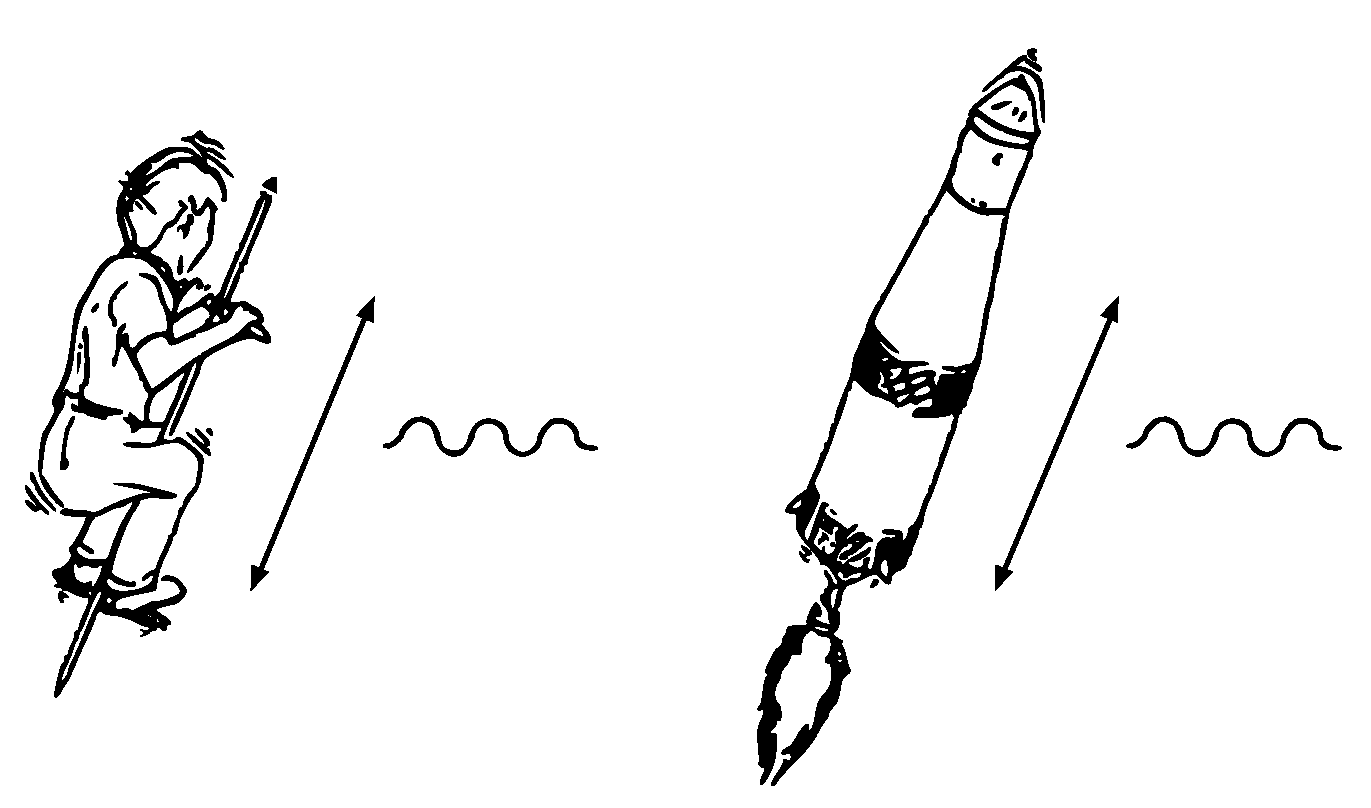
\includegraphics[width=.65\linewidth]{POGO-Analog}
  \caption{POGO比拟示意图}\label{POGO-Analog}
\end{figure}

\begin{figure}[th]
  \centering
  \includegraphics[width=.75\linewidth]{POGO-Typical.pdf}
  \caption{典型纵向耦合振动的时域历程}\label{Typical:POGO}
\end{figure}

纵观现代火箭工程发展史,POGO振动有害于人类航天飞行的典型例证当属美国土星V运载器的一系列发射经历\cite{Hill:1969, Rich:1969, Jarvinen:1970}。土星V运载火箭是美国最大的运载器,是美国国家航空航天局(NASA)在阿波罗计划和天空实验室两项太空计划中使用的多级可抛式液态燃料火箭。事实上,在其总共多达十三次的发射经历中,数次都受到了POGO振动问题的困扰\cite{Larsen:2008}。在1968年土星V编号AS-502次的发射过程中,液体火箭一级推进器(图\ref{SaturnV-Stage1})在工作段105$\sim$140秒内发生了振动频率为5.3Hz,幅值约0.33g的POGO振动。振动导致了五个发动机推力不同步,最终使得飞船登月舱裙部壁板发生开裂。同年十二月发射的土星AS-503,在发动机关机前50秒出现了振动频率为18Hz的POGO振动。事后调查表明,此次主发动机机架与贮箱底部产生的谐振虽然没有传递到火箭壳体,但是已经非常接近简体结构的设计强度极限。在1969年第AS-507次飞行中,液体火箭二级发动机在工作期间出现了四次严格意义上的POGO 振动,所幸最终都被结构系统的非线性效应所遏制。然而,在1970年土星V执行阿波罗13号任务的时候(AS-508),严重的POGO振动导致主发动机机架产生了频率为16Hz,加速度高达68g的失稳现象。由于燃烧室内压力脉动过于剧烈,火箭中部的5号推进器在二级火箭燃烧过程中发生了提前关闭(图\ref{SaturnV-Stage1}),最终导致登月任务被迫放弃,调查发现发动机机架总共被拉长了约7.6厘米。除此之外,宇宙神、大力神和雷神等航空运载器也都在各自发射过程中出现了或多或少的POGO振动\cite{Walker:1964, Wagner:1970, Oppenheim:1993};而法国钻石B火箭更是在其初次发射的五次飞行中都遇到了POGO振动,并且箭体上部分位置的振动量级已然高达足以导致运载器或者卫星结构发生破坏的20$\sim$30g\cite{Dordain:1974}。反观我国的航天事业,在2003年运载火箭长征2F第五次飞行中,遥测数据与宇航员的感受均显示一级助推器飞行末期火箭产生了比较强烈的振动\cite{Ma-Daoyuan:2010, Rong-Kelin:2011}。

\begin{figure}[t]
  \begin{center}
  \begin{minipage}{.47\linewidth}
    \includegraphics[width=\linewidth]{SaturnV-Stage1.jpg}
    \caption{土星V一级推进器 S-IC}\label{SaturnV-Stage1}
  \end{minipage}
  \begin{minipage}{.47\linewidth}
    \includegraphics[width=\linewidth]{SaturnV-Stage2.jpg}
    \caption{土星V二级推进器提前关闭}\label{SaturnV-Stage2}
  \end{minipage}
\end{center}
\end{figure}

POGO振动的危害性主要表现在如下几个方面\cite{Rubin:1970, Wang-Qizheng:1999}:
\begin{enumerate}[leftmargin=\parindent, align=parleft, labelindent=0pt, labelwidth=*]
\item 可使运载器结构系统产生过大的动载荷,造成火箭有效载荷部分损坏,影响主要任务的完成。如法国的“钻石B”运载火箭。
\item 管路系统产生的脉动压力和脉动流量可以导致运载火箭性能降低,造成任务失败。由于燃烧室压力的剧烈振荡导致出现虚假的推进剂耗尽指示信号,致使发动机过早关车。如美国的“大力神”二号任务失败,“土星V/阿波罗13”运载火箭第二级性能大大降低。
\item 增加运载器结构载荷,使有效载荷重量受到限制,而不得不重新设计结构。如美国的“雷神/阿金纳”火箭重新设计了“阿金纳”的结构。
\item 可以导致仪器、惯性仪表、设备和卫星所不允许的振动环境条件。如“雷神/阿金纳”运载火箭“阿金纳”级上的仪器设备需按较大的正弦振动等级重做安全鉴定。
\item 可以产生宇航员所不能允许的振动条件,使得宇航员的生理系统失调、身体不适,进而不能正常工作。如“双子星座/大力神”运载火箭的宇航员视力模糊,感到不舒服。
\end{enumerate}

根据NASA等机构对人体的测试表明\cite{Creer:1960, Burton:1988, Davis:2008}:垂直状态下正常人体所能承受的G力极限为5g,经过训练的宇航员可以短时承受正9g的最大加速度;在水平方向上,早期实验表明未经训练的人员在20g的加速度下只能坚持少于十秒的时间,10g可以支持一分钟,6g状态则能够维持十分钟。一般来说,短暂的“红视症”(Blackout,负G力)与“黑视症”(Redout,正G力)只是人体自我保护机制产生的警讯,用以警告人体已经濒临极限。倘若继续维持甚至增加G力,脑部将再因保护机制而停止工作产生昏厥,此时位于空中的飞行器即有极度危险;接着,当G力超过人脑所能负荷极限时,人脑将因长时间过度缺氧或充血的血管破裂而造成永久性伤害,最严重的即是因脑部严重损坏而死亡,或是脆弱的内部组织因持续遭受高G力而产生破裂,造成严重出血并危及生命。

可以看出,能否成功抑制甚至消除POGO振动已经成为当代航天运载器的重要设计指标之一,也是人类能否进行宇航飞行的前提之一。所以,目前基本上所有研究大型液体火箭的国家都对这种振动给予了相当大的重视和研究力度。因此,在我国大力发展宇航事业的重大契机下,针对POGO振动稳定性方面的理论分析也变得更加紧迫和必要。

\section{纵向耦合振动问题的主要机理分析}
\label{sec:POGO_Mechanicsm}
从本质上讲,POGO振动是一种由于火箭结构系统和管路推进系统发生相互作用而引起的不稳定振动。这种振动带有明显的流固耦合低频振动特征,属于不稳定的闭环自激振动\cite{Rubin:1973, Doiron:1977, Huang-Huaide:1987}。

\begin{figure}[h]
  \centering
  \includegraphics[width=.6\linewidth]{Struture-Feedline-Interaction-Diagram.pdf}
  \caption{POGO振动示意框图}\label{Interaction-Diagram}
\end{figure}

除去一种不常见的增压气体耦合POGO振动\cite{Rubin:1970},典型的POGO闭环振动究其原因可以归纳为如下过程(图\ref{Interaction-Diagram}):在大型液体运载火箭飞行的过程中,燃烧剂和氧化剂输送管路内的液路压力和流量会因为火箭结构系统的扰动而产生脉动。此脉动量经过不同管路元件的层层传递,最终将会到达液体火箭燃烧室,进而引起发动机产生推力脉动。此外,在燃烧剂和氧化剂的输运过程中,管路系统也会由于液体和管壁发生流固耦合作用而产生作用于结构系统上的额外反馈力\cite{About:1987, Paidoussis:1993}。所以当发动机推力脉动,联合上述管路系统反馈力,作为外界扰动力反作用于箭体结构时,火箭结构系统和管路推进系统两者就有可能因为固有频率相接近而产生不断放大耦合作用,从而导致液体推进火箭产生自激的纵向不稳定振动\cite{Rubin:1970, Oppenheim:1993}。

\begin{figure}[!htb]
  \centering
  \includegraphics[width=\linewidth]{telemetry-typical.pdf}
  \caption{土星V箭体加速度传感器数据}\label{telemetry-typical}
\end{figure}

参考POGO振动的发生机理并结合国内外大量的飞行遥测数据\cite{Feng-Zhenxing:1981},可以知道这种不稳定振动的发生频率大多与火箭结构系统的低阶纵向振动频率较为接近,其产生和发展过程也表现的十分突然和强烈。事实表明,POGO振动可能发生在液体火箭飞行过程的各个时刻,一次发射也确实可能会出现多次的POGO 振动\cite{Larsen:2008}。然而,由于液体火箭飞行过程是一个持续的变结构参数过程,并且箭体结构在发生较大变形时所引起的非线性效应会打破上面描述的这种频率耦合,所以即使出现POGO 现象,箭体振动的幅值也不会一直发散,而是在其响应时间的历程记录曲线上会出现一个先增大后减小的“鼓包”,典型的遥测POGO振动图像如图\ref{telemetry-typical}所示。鉴于POGO振动从发生到完全消失的时间可能长达数十秒,并且由其引起的箭体纵向振动加速度幅值可能在有效载荷处高达十几甚至几十倍于重力加速度,所以POGO振动对于液体火箭所造成的影响需要根据这种自激振动的量级及持续的时间来进行评价\cite{Wang-Qizheng:1999}。



\section{本文的主要工作}

\begin{figure}[!b]
  \centering
  \includegraphics[width=.85\linewidth]{Inter-connect.jpg}
  \caption{神舟十号与天宫一号交汇对接示意图}\label{China-Manned-Flight}
\end{figure}

液体火箭纵向耦合振动问题是一个相对古老却又富含新鲜挑战和契机的复杂系统问题。在我国大力发展航空事业的今天(图\ref{China-Manned-Flight}),更被赋予了深层次的时代意义。传统的液体火箭POGO稳定性分析方法主要分为了矩阵法、单传法和临界阻尼法\cite{Wang-Qizheng:1999}等几类。这些方法都需要先计算出耦合系统的闭环或者开环传递函数,然后通过对系统传递函数进行特征值求解或者绘制Bode和Nyquist图等手段来进行POGO稳定性分析。不过,由于耦合系统的传递函数通常都包含了一些复杂的非线性函数,所以POGO稳定分析的理论难点其实可以被归结为如何快速精确地计算出复杂传递函数的特征值这一经典问题。以矩阵法为例,由于系统反馈力传递矩阵中的元素包含了超越函数和高阶多项式,所以需要对不对称的复数传递矩阵进行非线性复特征值求解,而通常这种非线性方程的求解过程都十分困难并且容易漏根\cite{Dennis:1983, Golub:1996}。正是考虑到此类特征值问题的复杂性,Oppenheim\cite{Oppenheim:1993}等人如前所述,尝试了利用有限元法对管路系统进行直接建模。事实证明,这种方法在处理简单液路元件的组装计算方面确实具有着很高的可操作性和精确度。然而,由于管道内的流体运动问题归根结底是一个复杂的非线性问题\cite{Munson:1990, Paidoussis:1993, Morand:1995},所以当简单流体模型不能够精确描述管路系统传递关系,而研究者们必须要考虑诸如边界层效应,甚至湍流等复杂流体运动的时候,经典的有限元方法就必须被进一步拓展才能适应研究需要,而这种扩展可能相比于直接求解非线性特征值问题更加棘手。除此之外,由于流体单元本构关系的构建严重依赖于液路元件实验参数(如液路惯性,阻抗等)的精确标定,而相比于直接测定各类液路元件的工作参数,标定管路系统的总体反馈力传递函数可能会显得更加方便并且直接。所以,本文在POGO稳定性求解方法的研究方面,直接针对于管路系统的反馈力传递函数展开分析,开辟了另外一种与液路元件有限元组装法平行的POGO振动问题快速特征值求解方法。

为了解决上述主要问题,本文将研究工作分为了以下三个部分:

\begin{enumerate}[label=\textbf{\Roman*.}, align=left, leftmargin=0pt, listparindent=\parindent, itemindent=!, labelwidth=\parindent, labelsep=0pt, itemsep=1em]
\litem{集中参数模型的POGO稳定性分析(第二章)} 本章主要介绍了液体火箭结构系统和管路推进系统典型液路元件的集中参数模型建模方法,发展了一种基于矩阵法和有理分式拟合法的耦合系统快速特征值求解算法。首先推导了各类管路元件上下游脉动压力、流量之间的传递函数关系,结合发动机燃烧室的压力平衡条件与贮箱底部实际边界条件,综合分析出了管路系统反馈于结构系统的力传递函数。接下来,利用快速特征值求解方法,将包含超越函数的管路推进系统反馈力传递函数等效变换为与结构动力学方程一致的形式,通过求解矩阵特征值问题确定了耦合系统的动力学稳定性问题。最后,通过与传统矩阵法进行计算结果和效率方面的比对,验证了该方法的可靠性和高效性。
\litem{基于三维带液贮箱模型的POGO稳定性分析(第三章)} 为了更好的模拟火箭贮箱内液体和结构系统之间的流固耦合效应,引入液体火箭贮箱的三维轴对称模型建模方法,并利用虚质量法对贮箱内的液体进行动力学比拟。发展后的三维带液贮箱模型为管路系统提供了更为科学和精确的入口端边界条件,可以同样利用第二章中描述的管路系统类结构化建模方法,结合MSC.Nastran提供的传递函数TF卡建模工具,将拟合完毕的管路系统传递函数与不同类型的结构系统模型进行耦合计算。通过直接计算耦合系统的复特征值问题,可以方便的得知耦合系统的POGO稳定性。此外,计算过程还考虑了POGO稳定性分析中的另外一项关键性技术,即结构系统阻尼特性的识别和建模。带液贮箱的模态实验表明:在满箱、半箱和空箱等不同状态下,火箭结构系统的阻尼特性存在着较大差异,且半箱状态下结构阻尼较其他状态有明显增大。通过调整贮箱干/湿面材料随时间变化的比例阻尼系数,计算模型成功模拟了上述模态实验结果。最终,通过与实际火箭发射的遥测数据进行对比,证明了本套方法可以快速准确的得出POGO出现时间和振动特性。
\litem{液体火箭POGO稳定性参数分析及传递特性分析(第四章)} 通过比较不同工况下液体火箭POGO稳定性分析结果,本章首先揭示了耦合系统特征值与管路系统关键参数(如蓄压器容积等)之间的相互联系。分析表明,作为POGO抑制器的蓄压器,其容积变化能够显著影响液体火箭管路系统的固有频率,继而改变耦合系统的POGO稳定性。此外,通过比较不同类型液体火箭的历史遥测数据,可以发现有效载荷(如卫星等)的实际振动状态与液体火箭整体POGO振动的强弱并不存在简单的线性关系,单纯的耦合系统特征值计算并不能完全展现液体火箭各处的真实振动状态。文章最后指出,若要使得POGO稳定性分析能够给予未来的发射任务以实质性指导意见,还需综合考虑耦合系统的加速度传递特性分析。
\end{enumerate}

%% !TEX encoding = UTF-8 Unicode
%!TEX TS-program = xelatex

\chapter{集中参数模型的POGO稳定性分析}

\section{液体火箭管路推进系统集中参数模型}
\label{sec:Lumped-Feedline-Model}
\begin{figure}[!htb]
	\centering
	\begin{minipage}[b]{0.3\textwidth}
		\centering
		\includegraphics[width=1.2in]{Straight-Tube.pdf}
		\caption*{(a) 输液直管}
	\end{minipage}
	\centering
	\begin{minipage}[b]{0.3\textwidth}
		\centering
		\includegraphics[width=1in]{Bellow.pdf}
		\caption*{(b) 波纹管}
	\end{minipage}
	\centering
	\begin{minipage}[b]{0.3\textwidth}
		\centering
		\includegraphics[width=1.5in]{Accumulator.pdf}
		\caption*{(c) 蓄压器}
	\end{minipage}
	\centering
	\begin{minipage}[b]{0.3\textwidth}
		\centering
		\includegraphics[width=1.6in]{Thrust.pdf}
		\caption*{(d) 推力室}
	\end{minipage}
	\centering
	\begin{minipage}[b]{0.3\textwidth}
		\centering
		\includegraphics[width=1in]{Multiplex.pdf}
		\caption*{(e) 多通连接器}
	\end{minipage}
	\centering
	\begin{minipage}[b]{0.3\textwidth}
		\centering
		\includegraphics[width=1.7in]{Pump.pdf}
		\caption*{(f) 发动机泵}
	\end{minipage}
	\caption{液体火箭管路系统典型元件}
	\label{FeedLine-TypicalElement}
\end{figure}

液体推进火箭的管路系统主要由抽吸管路、多通接头、泵、泵后管路、燃烧室、推力室、蓄压器等几部分组成(如图\ref{FeedLine-TypicalElement})。分析液体火箭流体系统动特性的方法有很多,这里采用工程上常用的集中参数分析法,又称LRC等效电路分析法\cite{Dimaggio:1972, Vaage:1972, YangMing:2010}。本节主要针对包含四管发动机的推进系统展开分析。假设四管发动机系统的结构是对称的,并且流体的流动状态也是对称的,可以将四管发动机系统简化为单管发动机系统进行处理。单管发动机管路系统各元件之间脉动压力和脉动流量的传递关系如图\ref{POGO-PipeLine}所示。

\begin{figure}[!htb]
  \centering
  \includegraphics[width=.9\linewidth]{PipeLines.pdf}
  \caption{液体火箭管路-结构耦合系统传递关系示意图}\label{POGO-PipeLine}
\end{figure}

\begin{enumerate}[label=\textbf{\Roman*.}, align=left, leftmargin=0pt, listparindent=\parindent, itemindent=!, labelwidth=\parindent, labelsep=0pt, itemsep=1em]
\litem{输液直管}
由于通常情况下输液直管的直径与长度之比很小,所以在研究其低频振动时,可以不考虑管两端的复杂现象,仅考虑液体的一维流动。管中液体的扰动可以用欧拉方程和连续性方程来描述:
\begin{align}
	\frac{\partial v}{\partial t}+{{v}_{0}}\frac{\partial v}{\partial x}+\frac{1}{\rho }\frac{\partial p}{\partial x}&=0 \nonumber \\
	\frac{\partial p}{\partial t}+{{v}_{0}}\frac{\partial p}{\partial x}+c_{0}^{2}\rho \frac{\partial v}{\partial x}&=0
\end{align}
其中$v_0,c_0$为未扰动流的速度和当地声速,$p(x,t),v(x,t)$为流体的脉动压力和脉动速度。对上式进行求解,经过推导可以得到如下的输液直管上、下游脉动压力和流量之间的传递关系式:
\begin{equation}
	\label{eq:Straight-Tube}
	\left[ \begin{matrix}
	   {{P}_{2}}  \\
	   {{Q}_{2}}  \\
	\end{matrix} \right]=\left[ \begin{matrix}
	   \cosh \left( \theta  \right) & {\displaystyle -\frac{Z\sinh \left( \theta  \right)}{\theta }}  \\
	   {\displaystyle -\frac{\theta \sinh \left( \theta  \right)}{Z}} & \cosh \left( \theta  \right)  \\
	\end{matrix} \right]\left[ \begin{matrix}
	   {{P}_{1}}  \\
	   {{Q}_{1}}  \\
	\end{matrix} \right]
\end{equation}
式中$Z=sL+R,L=\rho l/A,\tau =lc,\theta^2=s^2\tau^2Z/(sL)$,其中$l$为管路长度,$Z$为液路阻抗,$L$为液路惯性,$R$为液路阻力,$c$为当地声速,$\rho$为液体密度,$s$为拉普拉斯变量,$A$为管路截面积。

\litem{蓄压器动力学模型}蓄压器是典型的POGO振动抑制器件,这里主要介绍目前国内外广泛应用的被动封闭式蓄压器,其简化物理模型如图\ref{FeedLine-TypicalElement}(c)所示。这种蓄压器包括了气腔和液腔,假设内部气体满足多方气体定律$P_gV_g^{\gamma}=C_g$,模拟输液直管传递关系的推导方法,可以得出其如下的传递关系:
\begin{equation}
\left[ \begin{matrix}
   {P_2}  \\
   {Q_2}  \\
\end{matrix} \right]=\left[ \begin{matrix}
   1 & 0  \\
   -Y & 1  \\
\end{matrix} \right]\left[ \begin{matrix}
   {P_1}  \\
   {Q_1}  \\
\end{matrix} \right]
\end{equation}
记蓄压器阻抗为$Z$、导纳为$Y$
\begin{align}
	Z&=\frac{s^2CL+sCR+1}{sC} \nonumber\\
	Y&=\frac{1}{Z}=\frac{s}{\displaystyle L\left(s^2+2\zeta\omega s+\omega^2 \right)} \nonumber
\end{align}
其中$\omega=\sqrt{1/CL},\zeta=CR\omega/2$,$C$为蓄压器柔度,$R$和$L$意义同上。
\end{enumerate}

至此,可以利用上述管段元件的传递关系进行液体火箭管路系统的总体传递矩阵组装(矩阵记号参考图\ref{POGO-PipeLine})
\begin{equation}
	\boldsymbol{\mathbb{T}}=\boldsymbol{T}^6\boldsymbol{T}^5\boldsymbol{T}^4\boldsymbol{T}^3\boldsymbol{T}^2\boldsymbol{T}^1=\left[ \begin{matrix}
	   {T}_{11} & {T}_{12}  \\
	   {T}_{21} & {T}_{22}  \\
	\end{matrix} \right],\; 
	\boldsymbol{T}^s=\boldsymbol{T}^6 \left[ 
	\begin{matrix}
	   -A_{L1}^{(5)}Z_{L1}^{(5)}  \\
	   A_{L1}^{(5)}  \\
	\end{matrix} \right] = \left[ \begin{matrix}
	   {T}_{1}^s  \\
	   {T}_{2}^s  \\
	\end{matrix} \right]
\end{equation}
考虑管路系统入口处脉动压力和脉动流量与箱底振动速度之间的关系:
\begin{equation}
	\label{eq:Inlet-Boundary-Condition}
	P_{L1}^{(1)}=s\rho{h}_T\left(1-\frac{A_{L1}^{(1)}}{A_T}\right){\dot{x}_T}(s)- \frac{s\rho{h_T}Q_{L1}^{(1)}}{A_T}
\end{equation}
其中,符号下标${}_{L1},{}_{L2}$用于区分管路参数描述位置(入口或出口),数字上标${}^{(n)}$表示该参数描述第$n$段管路元件, $h_T$为贮箱液面高度,$A_{L1}^{(1)}, A_T$分别表示与贮箱底部相连管路的截面积和贮箱截面积,$\dot{x}_T$表示箱底扰动速度。

结合发动机燃烧室内的压力上下游平衡关系$P_{L1}^{(7)}=P_{L2}^{(6)}$,经过一系列换算,最终可以得到管路系统初始脉动压力$P_{L1}^{(1)}$和脉动流量$Q_{L1}^{(1)}$与箱底扰动速度$\dot{x}_T$和泵位置扰动速度$\dot{x}_{L1}^{(5)}$之间的传递关系:
\begin{align}
  \label{eq:Total-Transfer}
  Q_{L1}^{(1)}=&\frac{\left( {T}_{1}^{s}-Z_{L1}^{(7)} {T}_{2}^{s} \right)\dot{x}_{L1}^{(5)}(s)- s{\rho}{h_T}\left( 1- {\displaystyle \frac{A_{L1}^{(1)}}{A_T}} \right) \left( Z_{L1}^{(7)} {T}_{21}- {T}_{11} \right) {\dot{x}_T(s)} } {Z_{L1}^{(7)} {T}_{22}- {T}_{12}- {\displaystyle \frac{s\rho h_T}{A_T}} \left( Z_{L1}^{(7)} {T}_{21}- {T}_{11} \right)} \nonumber\\
  %%%
  P_{L1}^{(1)}=% 
  &-\frac{s\rho{h_T}}{A_T} \left[
  \frac{\left( {T}_{1}^{s}-Z_{L1}^{(7)} {T}_{2}^{s} \right)\dot{x}_{L1}^{(5)}(s)- s{\rho}{h_T}\left( 1- { \frac{A_{L1}^{(1)}}{A_T}} \right) \left( Z_{L1}^{(7)} {T}_{21}- {T}_{11} \right) {\dot{x}_T(s)} } {Z_{L1}^{(7)} {T}_{22}- {T}_{12}- { \frac{s\rho h_T}{A_T}} \left( Z_{L1}^{(7)} {T}_{21}- {T}_{11} \right)}
  \right] \nonumber\\
  &+ s\rho{h}_T \left(1- \frac{A_{L1}^{(1)}}{A_T}\right){\dot{x}_T}(s)
\end{align}

通常,作用在液体火箭上的典型外力主要包括了以下几类:\label{Page:Typical-Feedback-Force}
\begin{enumerate}[leftmargin=\parindent, align=parleft, labelindent=0pt, labelwidth=*]
\item 贮箱底开口处相对脉动流出量引起贮箱液体质心脉动对结构作用力。
\begin{equation}
	F_1=\rho h_Ts \left[ Q_{L1}^{(1)}+ A_{L1}^{(1)}\dot{x}_T(s) \right]
\end{equation}
\item 贮箱底开口处的脉动压力对结构作用力。
\begin{equation}
	F_2=A_{L1}^{(1)}P_{L1}^{(1)}
\end{equation}
\item 泵前后压力动量变化对结构作用力。
\begin{equation}
	F_3=N\left[ -A_{L1}^{(4)}P_{L1}^{(5)}- \rho Q_s \left( \frac{2Q_{L1}^{(5)}}{A_{L1}^{(4)}}+ \dot{x}_{L1}^{(5)}(s) \right)\right]
\end{equation}
\item 发动机燃烧室脉动压力引起脉动推力。
\begin{equation}
	F_4=NA_{th}C_f P_{L2}^{(7)}
\end{equation}
\end{enumerate}
其中,$A_{L1}^{(4)}$表示泵上游入口处截面积,$Q_s$表示泵的稳态体积流,$N$表示发动机台数,$A_{th}$为发动机喉部截面积,$C_f$为有效推力系数。

利用公式\eqref{eq:Total-Transfer},可以把管路推进系统作用到结构上的反馈力表示为:
\begin{equation}
	\label{eq:Feedback-Force-Transfer}
	\boldsymbol{F}_p(s)=\left[ \begin{matrix}
	   F_1(s)  \\
	   F_2(s)  \\
	   F_3(s)  \\
	   F_4(s)  \\
	\end{matrix} \right]  \triangleq \boldsymbol{R}_{pq}(s)\left[ \begin{matrix}
	   \dot{x}_T(s)  \\
	   \dot{x}_{L1}^{(5)}(s)  \\
	\end{matrix} \right] \triangleq \boldsymbol{R}_{pq}(s)\boldsymbol{\dot{X}}_q(s)
\end{equation}
矩阵$\boldsymbol{R}_{pq}(s)$代表了箭体振动速度$\boldsymbol{\dot{X}}_q(s)$与推进系统反馈力$\boldsymbol{F}_p(s)$之间的传递关系。可以看出,该速度阻抗矩阵形式复杂,且包含了难以处理的超越函数。

\section{液体火箭结构系统集中参数模型}
\label{sec:Lumped-Rocket-Structural-System}
\begin{figure}[!htb]
  \centering
  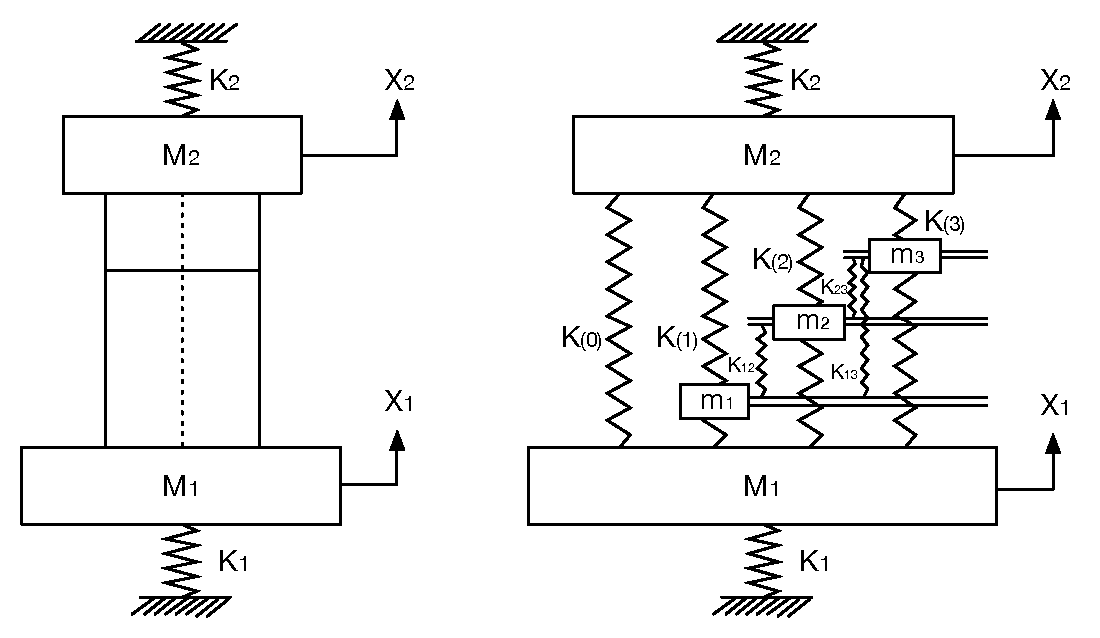
\includegraphics[width=.8\linewidth]{Lumped-Mass-Spring-Glaser}
  \caption{液体贮箱集中参数Glaser弹簧-质量模型}\label{Lumped-Mass-Spring-Glaser}
\end{figure}

\begin{figure}[p]
  \centering
  \centerline{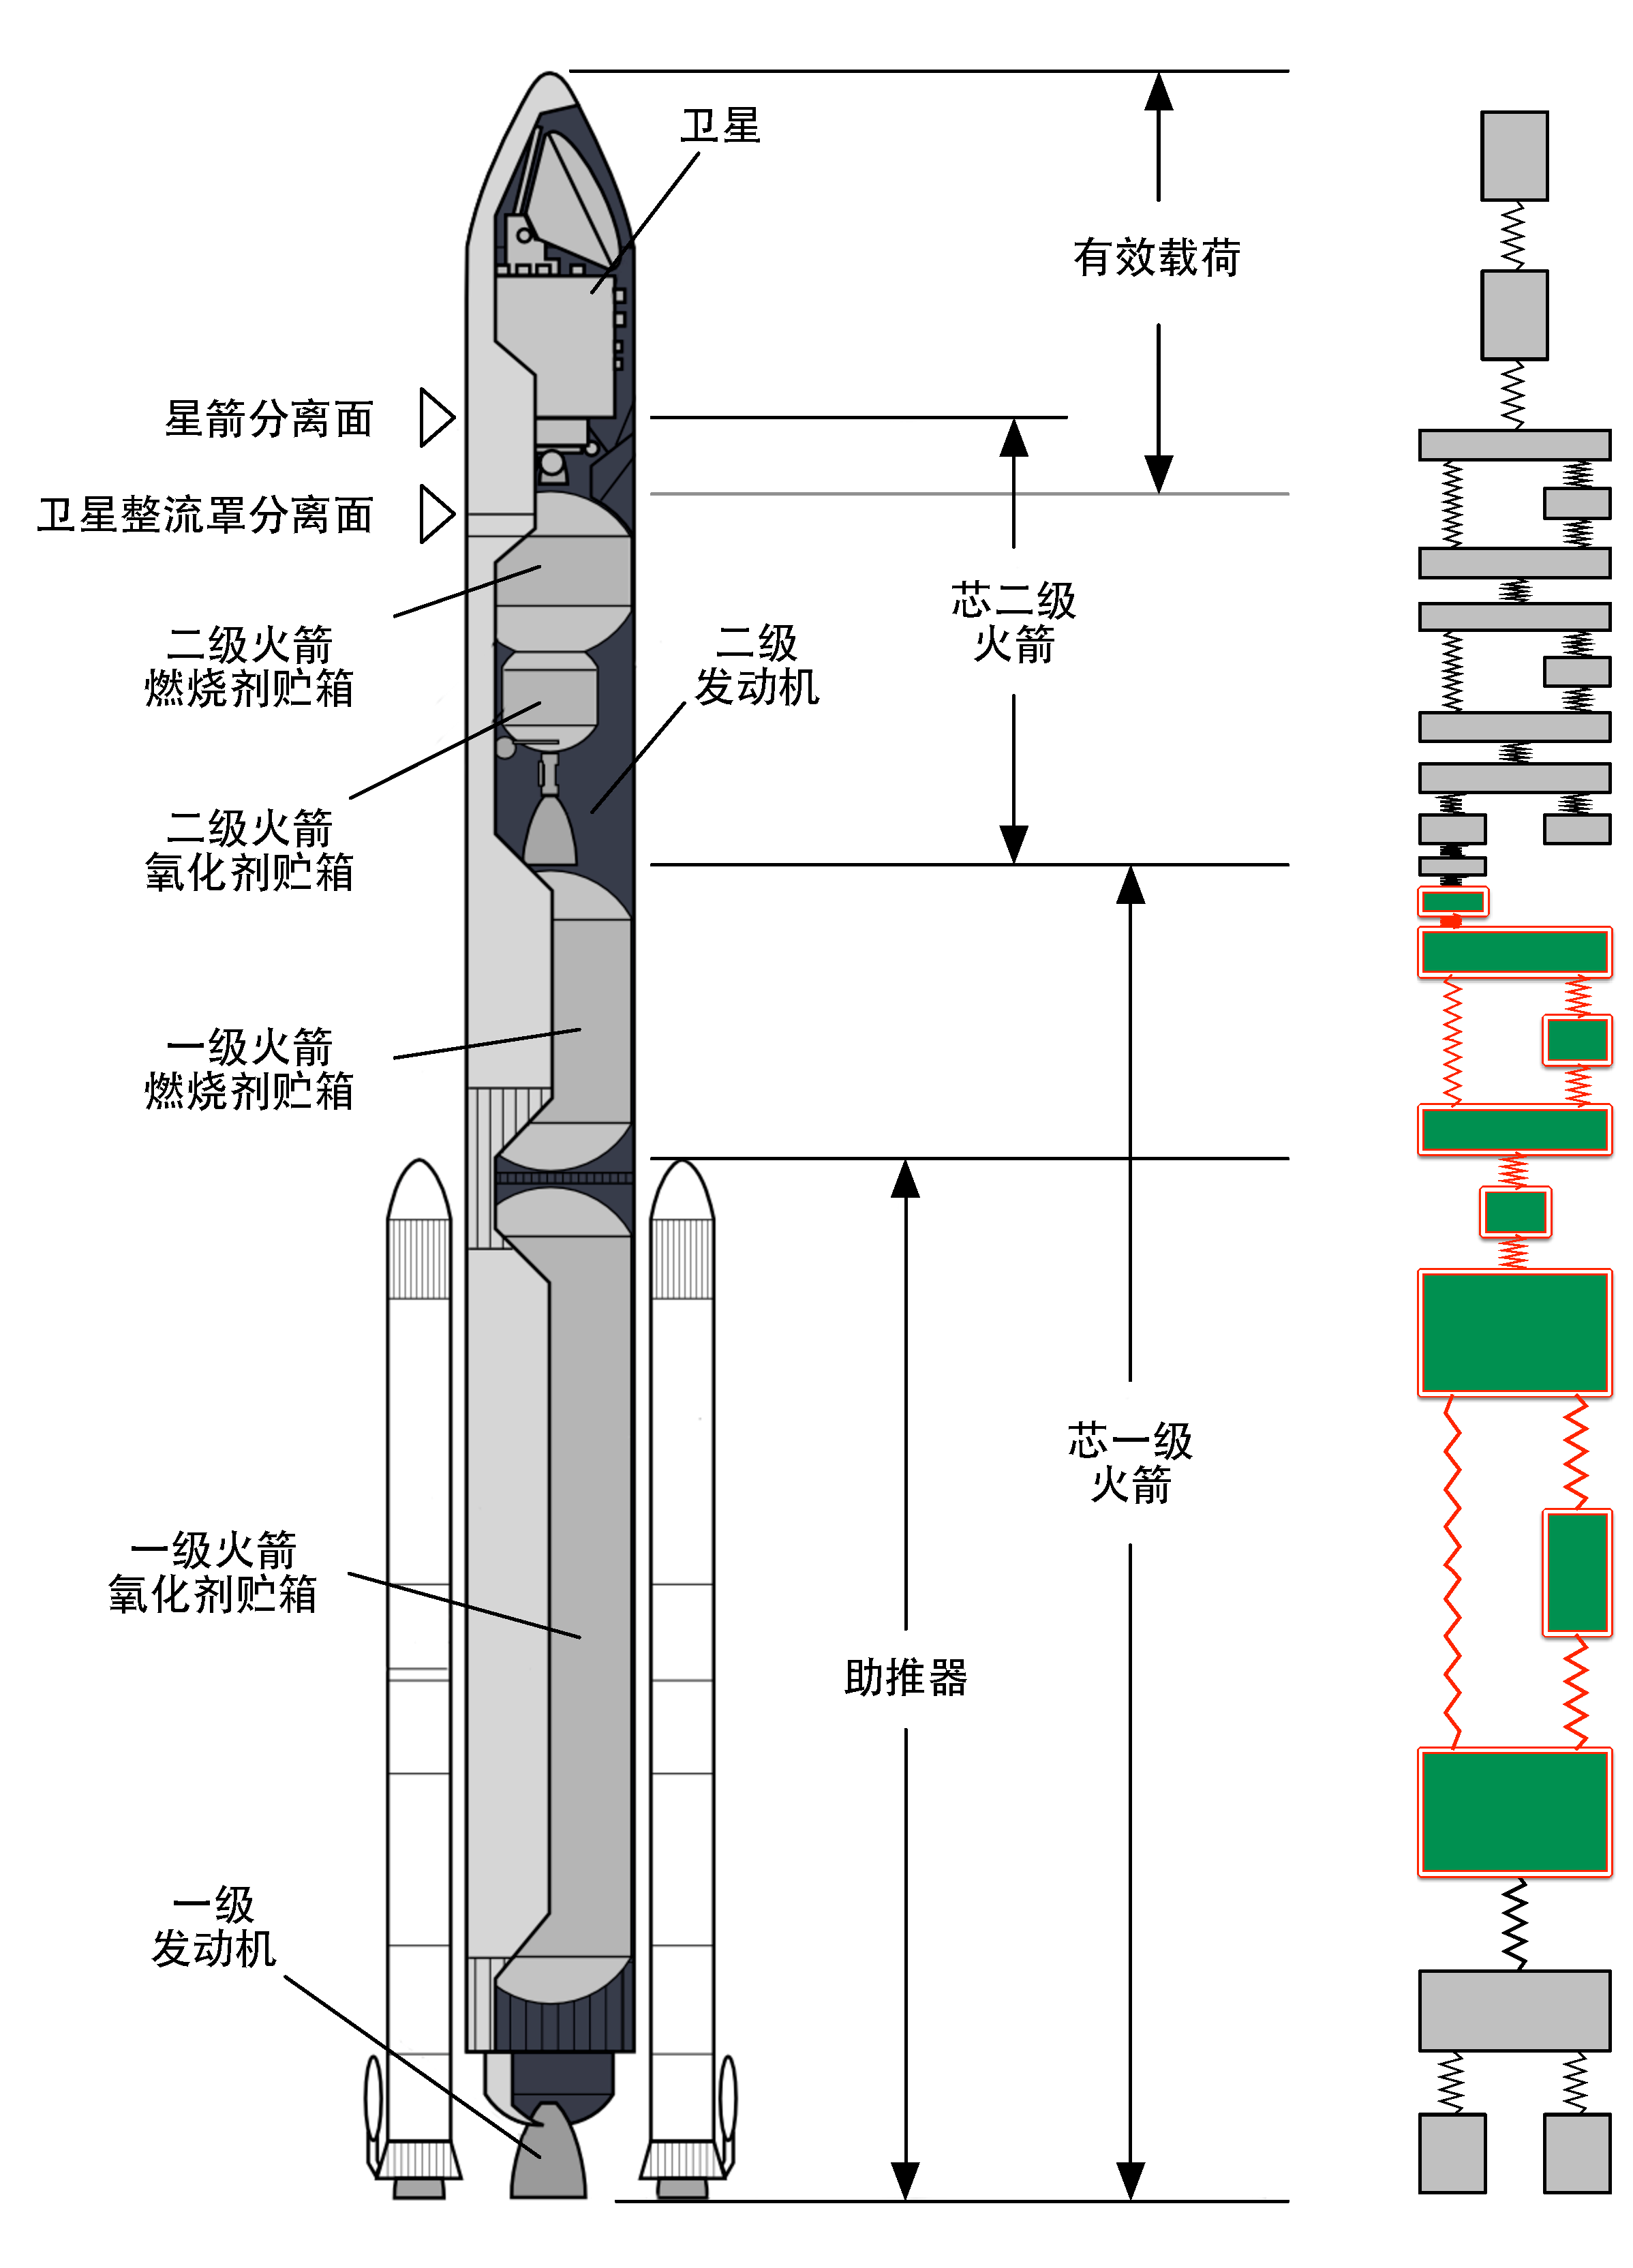
\includegraphics[width=.95\linewidth]{Whole-Rocket-Model}}
  \caption{液体火箭全箭集中质量模型}\label{Whole-Rocket-Model}
\end{figure}

\section{耦合系统稳定性分析方法}
传统的液体火箭POGO稳定性分析方法主要分为了矩阵法、单传法和临界阻尼法\cite{Wang-Qizheng:1999}等几类。从现代控制理论的角度出发\cite{Ogata:2009},这些方法从本质上看都是通过求解系统特征值来判断系统是否稳定:耦合系统特征值出现正实部则系统不稳定,若特征值实部全为负数则系统稳定。其中,矩阵法可分为闭环分析法和开环分析法,是传统POGO稳定性分析方法中最复杂、精度最高的。其余两种方法虽然计算过程较为简单,但由于计算结果精度较差,所以研究者们逐渐的将目光转向了更能满足目前工况计算要求的新型稳定性分析方法。本节将引入一种基于矩阵法的新型POGO稳定性快速求解方法。

根据公式\eqref{eq:Feedback-Force-Transfer}和\eqref{eq:Structure-Dynamic-Freq},可以把耦合系统的频域特征方程表示为:
\begin{equation}
	\label{eq:Coupled-System-Transfer-TMP}
	\left[s^2 \boldsymbol{M}_s+ s(\boldsymbol{C}_s+\boldsymbol{\dot{M}}_s)+ \boldsymbol{K}_s \right]\boldsymbol{X}_s(s)=\boldsymbol{F}_s(s)+ \boldsymbol{L}_{sp} \boldsymbol{R}_{pq}(s)\boldsymbol{\dot{X}}_q(s)
\end{equation}
若引入转换结构系统速度反馈节点位置的布尔矩阵,
\begin{displaymath}
	\boldsymbol{x}_q(t)=
	\left[ \begin{matrix}
		{x}_T(t) & {x}_{L1}^{(5)}(t)
	\end{matrix} \right]^{\ut}=
	\boldsymbol{L}_{qs} \boldsymbol{x}_s(t)
\end{displaymath}
可将公式\eqref{eq:Coupled-System-Transfer-TMP}改写为:
\begin{equation}
	\label{eq:Coupled-System-Transfer}
	\left[s^2 \boldsymbol{M}_s+ s\left(\boldsymbol{C}_s+\boldsymbol{\dot{M}}_s
	-\boldsymbol{L}_{sp} \boldsymbol{R}_{pq}(s)\boldsymbol{L}_{qs}\right)+ \boldsymbol{K}_s \right]\boldsymbol{X}_s(s)=\boldsymbol{F}_s(s)
\end{equation}
耦合系统稳定的准则是如下代数方程根的实部均不大于零:
\begin{equation}
	\label{eq:Coupled-Transfer-Det}
	\Psi (s) \triangleq \det
	\left[s^2 \boldsymbol{M}_s+ s\left(\boldsymbol{C}_s+\boldsymbol{\dot{M}}_s
	-\boldsymbol{L}_{sp} \boldsymbol{R}_{pq}(s)\boldsymbol{L}_{qs}\right)+ \boldsymbol{K}_s \right]\boldsymbol{X}_s(s)=0
\end{equation}

\subsection{反馈力传递函数的有理分式拟合方法}
从公式\eqref{eq:Coupled-Transfer-Det}的形式可以看出,耦合系统特征值问题的求解难点主要缘于阻抗函数$\boldsymbol{R}_{pq}(s)$的形式较为复杂。所以本节主要研究如何将其进行合理的等效变换,将包含了诸如双曲函数形式的管路系统反馈力传递函数转化为便于与液体火箭结构系统进行耦合分析的有理分式形式。

如果只考虑阻抗矩阵$\boldsymbol{R}_{pq}(s)$的单个元素,可以利用有理分式将此单输入单输出(SISO)传递函数在频域拟合为如下标准形式\cite{Gustavsen:1999, Zeng:2006}:
\begin{equation}
	\label{eq:Standard-SISO-Freq}
	T(\jmath\omega)=\jmath\omega M_0+ D_0+ \sum_{k=1}^{n}\frac{C_k}{\jmath\omega-A_k}+ \sum_{k=1}^{n}\frac{\bar{C}_k}{\jmath\omega- \bar{A}_k}+ \sum_{j=1}^{m} \frac{B_j}{\jmath\omega -R_j}
\end{equation}

其中$\jmath=\sqrt{-1}$,$A_k, R_j$为已知的极点,$M_0, D_0, C_k, B_j$为待定系数,符号$\bar{}$表示对应变量的共轭。值得注意的是,此处考虑了有理分式中包含成对出现的共轭极点、纯实数极点、直流分量和一次项的广义情况,实际拟合过程可能只需要保留其中的部分项。

根据离散的传递函数数据,可以在$n_f$个频率点上建立如下方程:
\begin{equation}
	\label{eq:Discrete-Standard-Transfer}
	T(\jmath\omega_f)=\jmath\omega_f M_0+ D_0+ \sum_{k=1}^{n}\frac{C_k}{\jmath\omega_f-A_k}+ \sum_{k=1}^{n}\frac{\bar{C}_k}{\jmath\omega_f- \bar{A}_k}+ \sum_{j=1}^{m} \frac{B_j}{\jmath\omega_f -R_j}
\end{equation}
记
\begin{align}
	& \boldsymbol{m}_1(\omega_f)=\left[ \begin{matrix}
	   \jmath\omega_f & 1
	\end{matrix} \right] \nonumber\\
	& \boldsymbol{m}_2(\omega_f)=\left[ \begin{matrix}
	   \displaystyle{\frac{1}{\jmath \omega_f-A_1}} & \cdots & \displaystyle{\frac{1}{\jmath \omega_f-A_n}}  \\
	\end{matrix} \right] \nonumber\\ 
	& \boldsymbol{m}_3(\omega_f)=\left[ \begin{matrix}
	   \displaystyle{\frac{1}{\jmath \omega_f-\bar{A}_1}} & \cdots & \displaystyle{\frac{1}{\jmath \omega_f-\bar{A}_n}}  \\
	\end{matrix} \right]  \\ 
	& \boldsymbol{m}_4(\omega_f)=\left[ \begin{matrix}
	   \displaystyle{\frac{1}{\jmath \omega_f-R_1}} & \cdots & \displaystyle{\frac{1}{\jmath \omega_f-R_m}} \\ 
	\end{matrix} \right] \nonumber \\ 
	& \boldsymbol{C}=\left[ \begin{matrix}
	   C_1 & \cdots & C_n
	\end{matrix} \right]^{\ut} \nonumber \\ 
	& \boldsymbol{B}=\left[ \begin{matrix}
	   B_1 & \cdots & B_m
	\end{matrix} \right]^{\ut} \nonumber
\end{align}
可以将公式\eqref{eq:Discrete-Standard-Transfer}改写为:
\begin{equation}
	T(\jmath \omega_f)=\boldsymbol{m}_1(\omega_f)\left[ 
	\begin{matrix} 
	M_0 \\
	D_0 \\
	\end{matrix} \right] + \boldsymbol{m}_2(\omega_f)\boldsymbol{C} + \boldsymbol{m}_3\boldsymbol{\bar{C}} +\boldsymbol{m}_4(\omega_f)\boldsymbol{B}
\end{equation}
将上式进行实部和虚部分离,方程变为
\begin{equation}
	\label{eq:SISO-Least-Square}
	\left[ \begin{matrix}
	   T'(\omega_f)  \\
	   T''(\omega_f)  \\
	\end{matrix} \right]=\left[ \begin{matrix}
		\boldsymbol{m}'_1(\omega_f) & \boldsymbol{m}''_1(\omega_f) \\
		\boldsymbol{m}'_2(\omega_f)+ \boldsymbol{m}'_3(\omega_f) & \boldsymbol{m}''_2(\omega_f)+ \boldsymbol{m}''_3(\omega_f) \\
		\boldsymbol{m}''_3(\omega_f)- \boldsymbol{m}''_2(\omega_f) & \boldsymbol{m}'_2(\omega_f)-\boldsymbol{m}'_3(\omega_f) \\
		\boldsymbol{m}'_4(\omega_f) & \boldsymbol{m}''_4(\omega_f) \\
		-\boldsymbol{m}''_4(\omega_f) & \boldsymbol{m}'_4(\omega_f)
	\end{matrix} \right]^{\ut} \left[ \begin{matrix}
	   M_0  \\
	   D_0  \\
	   \boldsymbol{C}'  \\
	   \boldsymbol{C}''  \\
	   \boldsymbol{B}'  \\
	   \boldsymbol{B}''  \\
	\end{matrix} \right]
\end{equation}
其中,复数变量的记号约定如下:
\begin{equation}
	\Re(T)=T',\quad\Im(T)=T''
\end{equation}
利用最小二乘法\cite{Bjorck:1996},可以根据公式\eqref{eq:SISO-Least-Square}求解出有理分式\eqref{eq:Standard-SISO-Freq}中的各项待定系数。此外,如果发现拟合结果在某些重要频率范围内的精度达不到标的要求,还可以利用加权的最小二乘法\cite{Strutz:2011}对求解过程进行适当优化。

对于POGO研究中所涉及到的多输入多输出(MIMO)系统,可以利用上述方法对于阻抗矩阵$\boldsymbol{R}_{pq}(s)$中的各个分量进行分别拟合。值得注意的是,根据通过理论推导可以得知:管路系统反馈力传递矩阵中各个分量的极点是相同的,所以在对传递函数进行最小二乘法拟合之前,只需选其任意一个分量进行极点探测即可。如果在极点探测的过程中出现了由于数值误差或者拟合精度设置不统一等因素导致的极点不一致情况,工程上也可以将分别拟合得到的极点进行平均化处理。至于有理多项式拟合应采用多少极点,可以先解析的绘制出阻抗矩阵$\boldsymbol{R}_{pq}(s)$各分量的传递函数图形,根据曲线峰值的数目进行多项式项数的预估,然后根据具体的拟合结果进行拟合迭代次数和极点个数等参数的微调,最终得出合理的拟合结果。

\begin{figure}[p]
  \centering
  \includegraphics[trim={4.5cm 0cm 4.5cm 0cm}, clip=true, width=\linewidth]{Fitted-Transfer-01.pdf}
  \caption{管路系统反馈力有理分式拟合前后对比曲线(a):$\boldsymbol{R}_{11}-\boldsymbol{R}_{41}$}
  \label{Rational-Fitted-VS-01}
  \vspace{1.2em}
  \includegraphics[trim={4.5cm 0cm 4.5cm 0cm}, clip=true, width=\linewidth]{Fitted-Transfer-02.pdf}
  \caption{管路系统反馈力有理分式拟合前后对比曲线(b):$\boldsymbol{R}_{12}-\boldsymbol{R}_{42}$}
  \label{Rational-Fitted-VS-02}
\end{figure}

至此,可以将推进系统作用到结构上的反馈力将表示为:
\begin{equation}
	\label{eq:Rational-Feedback-Force}
	\boldsymbol{F}_p(s)= \boldsymbol{R}_{pq}(s)\boldsymbol{\dot{X}}_q(s)
	=\left[ s\boldsymbol{M}_{pq}+ \boldsymbol{D}_{pq}+ \sum_{k=1}^n
	\left( \frac{\boldsymbol{C}_{pq}^{(k)}}{s-{A}_k} +
	\frac{\bar{\boldsymbol{C}}_{pq}^{(k)}}{s-\bar{A}_k}  \right)
	 \right] \boldsymbol{\dot{X}}_q(s)
\end{equation}
其中$\boldsymbol{M}_{pq}, \boldsymbol{D}_{pq}$为实矩阵,${A}_k$为成对的共轭极点,$\boldsymbol{C}_{pq}^{(k)}$为成对的共轭矩阵,$p,q$分别表示阻抗矩阵的行数和列数,既管路系统反馈力和结构系统速度反馈节点的个数。在通常情况下,由于振动分析很少关注传递函数中包含纯实极点的情况,所以在拟合反馈力传递函数的时候并没有添加$R_j$项。

\subsection{反馈力传递矩阵的类结构化建模}
经过上节有理分式的拟合过程,管路系统反馈力传递函数已经被表示为了形如公式\eqref{eq:Rational-Feedback-Force}的较为简单形式。接下来,考虑对其进行进一步等效变换,通过引入辅助变量将有理分式转化为与结构振动方程相似的二阶常微分方程形式,便于进行下一步的耦合系统快速特征值求解。为此,考察$\boldsymbol{R}_{pq}(s)$其中一对共轭项:
\begin{equation}
	\label{eq:Feedback-Force-Original}
	\boldsymbol{F}_p^{(k)}(s)=\left( \frac{\boldsymbol{C}_{pq}^{(k)}}{s-A_k}+ \frac{\bar{\boldsymbol{C}}_{pq}^{(k)}}{s-\bar{A}_k} \right) \dot{\boldsymbol{X}_q}(s)
\end{equation}
对矩阵$\boldsymbol{C}_{pq}^{(k)}$做奇异值分解\cite{Golub:1996}
\begin{equation}
	\label{eq:QR-Dissect}
	\boldsymbol{C}_{pq}^{(k)}=\boldsymbol{U}_{pp}^{(k)}\boldsymbol{S}_{pq}^{(k)}{\boldsymbol{V}_{qq}^{(k)}}^{*}
\end{equation}
此处${}^*$表示矩阵的共轭转置,$\boldsymbol{S}_{pq}^{(k)}$形式如下
\begin{equation}
	\label{eq:SVD-Rank-Analysis}
	\boldsymbol{S}_{pq}^{(k)}=\left[ \begin{matrix}
	   \boldsymbol{S}_{r_kr_k}^{(k)} & \boldsymbol{0}_{r_k(q-r_k)}  \\
	   \boldsymbol{0}_{(p-r_k)} & \boldsymbol{0}_{(p-r_k)(q-r_k)}  \\
	\end{matrix} \right]
\end{equation}
$r_k$为矩阵$\boldsymbol{C}_{pq}^{(k)}$的秩,$\boldsymbol{S}_{r_kr_k}^{(k)}$为非奇异实对角矩阵,$\boldsymbol{U}_{pp}^{(k)}, \boldsymbol{V}_{qq}^{(k)}$为复矩阵,满足:
\begin{equation}
{\boldsymbol{U}_{pp}^{(k)}}^*\boldsymbol{U}_{pp}^{(k)}=\boldsymbol{I}_{pp},
{\boldsymbol{V}_{qq}^{(k)}}^*\boldsymbol{V}_{qq}^{(k)}=\boldsymbol{I}_{qq}
\end{equation}
分别从矩阵$\boldsymbol{U}_{pp}^{(k)}, \boldsymbol{V}_{qq}^{(k)}$中取出前$r_k$列,构成列满秩矩阵$\boldsymbol{U}_{pr_k}^{(k)}, \boldsymbol{V}_{qr_k}^{(k)}$,将公式\eqref{eq:QR-Dissect}表示成
\begin{equation}
	\boldsymbol{C}_{pq}^{(k)}=\boldsymbol{U}_{pr_k}^{(k)}\boldsymbol{S}_{r_kr_k}^{(k)}{\boldsymbol{V}_{qr_k}^{(k)}}^{*}
\end{equation}
这样,可以将推进系统反馈力$\boldsymbol{F}_p^{(k)}(s)$改写为:
\begin{equation}
	\label{eq:Single-SVD-Feedback-Force}
	\boldsymbol{F}_p^{(k)}(s)=\left( \frac{
	\boldsymbol{U}_{pr_k}^{(k)}\boldsymbol{S}_{r_kr_k}^{(k)}{\boldsymbol{V}_{qr_k}^{(k)}}^{*}
	}{s-A_k}+ \frac{
	\boldsymbol{\bar{U}}_{pr_k}^{(k)}\boldsymbol{S}_{r_kr_k}^{(k)}{\boldsymbol{\bar{V}}}{{}_{qr_k}^{(k)}}^{*}
	}{s-\bar{A}_k} \right) \dot{\boldsymbol{X}_q}(s)
\end{equation}

\noindent 定义两组关于时间的实函数$\boldsymbol{y}_{r_k}^{\prime(k)}(t), \boldsymbol{y}_{r_k}^{\prime\prime(k)}(t)$,在时域满足微分方程
\begin{equation}
	\label{eq:Extra-Variable-ODE}
	\left\{ 
	\begin{aligned}
		\dot{\boldsymbol{y}}_{r_k}^{\prime(k)}(t)- A'_k\boldsymbol{y}_{r_k}^{\prime(k)}(t)+A''_k\boldsymbol{y}_{r_k}^{\prime\prime(k)}(t)&= {\boldsymbol{V}_{qr_k}^{\prime(k)}}^{\ut} \boldsymbol{x}_{q}(t)  \\ 
		\dot{\boldsymbol{y}}_{r_k}^{\prime\prime(k)}(t)-A''_k \boldsymbol{y}_{r_k}^{\prime(k)}(t)-A'_k\boldsymbol{y}_{r_k}^{\prime\prime(k)}(t)&= -{\boldsymbol{V}_{qr_k}^{\prime\prime(k)}}^{\ut} \boldsymbol{x}_{q}(t)
	\end{aligned} \right.
\end{equation} 
其中,复数变量的记号约定同上节:$A'_k=\Re(A_k),A''_k=\Im(A_k)$,复矩阵在写法上亦采用相同规范
\begin{displaymath}
	\boldsymbol{V}_{qr_k}^{\prime(k)}=\Re(\boldsymbol{V}_{qr_k}^{(k)}), \boldsymbol{V}_{qr_k}^{\prime\prime(k)}=\Im(\boldsymbol{V}_{qr_k}^{(k)})
\end{displaymath}
$\boldsymbol{x}_q(t)$是$\boldsymbol{X}_q(s)$的Laplace逆变换:
\begin{displaymath}
	\boldsymbol{x}_q(t)=\Lacelap{\boldsymbol{X}_q(s)}
\end{displaymath}
将公式\eqref{eq:Extra-Variable-ODE}进行Laplace变换,
\begin{equation}
	\label{eq:Extra-Variable-Laplace}
	\left\{ 
	\begin{aligned}
		(s-A'_k)\boldsymbol{Y}_{r_k}^{\prime(k)}(s)+ A''_k\boldsymbol{Y}_{r_k}^{\prime\prime(k)}(s)&={\boldsymbol{V}_{qr_k}^{\prime(k)}}^{\ut}\boldsymbol{X}_q(s) \\
		-A''_k\boldsymbol{Y}_{r_k}^{\prime(k)}(s)+ (s-A'_k)\boldsymbol{Y}_{r_k}^{\prime\prime(k)}(s)&= -{\boldsymbol{V}_{qr_k}^{\prime\prime(k)}}^{\ut}\boldsymbol{X}_q(s)
	\end{aligned} \right.
\end{equation}
其中
\begin{align}
	\boldsymbol{Y}_{r_k}^{\prime(k)}(s)&=\Laplace{\boldsymbol{y}_{r_k}^{\prime(k)}(t)} \nonumber \\
	\boldsymbol{Y}_{r_k}^{\prime\prime(k)}(s)&=\Laplace{\boldsymbol{y}_{r_k}^{\prime\prime(k)}(t)} \nonumber \\
	\boldsymbol{X}_q(s)&= \Laplace{\boldsymbol{x}_q(t)} \nonumber
\end{align}
可以验证,满足方程\eqref{eq:Extra-Variable-Laplace}的函数$\boldsymbol{Y}_{r_k}^{\prime(k)}, \boldsymbol{Y}_{r_k}^{\prime\prime(k)}$必然满足:
\begin{subequations}
	\label{eq:Extra-Variable-Laplace-Displacement}
	\begin{align}
		{\displaystyle\frac{{\boldsymbol{V}_{qr_k}^{(k)}}^{*}}{(s-A_k)}} \boldsymbol{X}_q(s)&= \boldsymbol{Y}_{r_k}^{\prime(k)}(s)+ \jmath\boldsymbol{Y}_{r_k}^{\prime\prime(k)}(s)  \label{eq:Extra-Variable-Laplace-Displacement-01}\\
		{\displaystyle\frac{\boldsymbol{\bar{V}}{{}_{qr_k}^{(k)}}^{*}}{(s-\bar{A}_k)}} \boldsymbol{X}_q(s)&= \boldsymbol{Y}_{r_k}^{\prime(k)}(s)- \jmath\boldsymbol{Y}_{r_k}^{\prime\prime(k)}(s)  \label{eq:Extra-Variable-Laplace-Displacement-02}
	\end{align}
\end{subequations}
将公式\eqref{eq:Extra-Variable-Laplace-Displacement}带入\eqref{eq:Single-SVD-Feedback-Force},$\boldsymbol{F}_p^{(k)}(s)$可以写为:
\begin{equation}
	\label{eq:Feedback-Single-Force-Extra-Variable}
	\boldsymbol{F}_p^{(k)}(s)=2\left[ \boldsymbol{U}_{pr_k}^{\prime(k)}\boldsymbol{S}_{r_kr_k}^{(k)} \dot{\boldsymbol{Y}}_{r_k}^{\prime(k)}(s)-
	\boldsymbol{U}_{pr_k}^{\prime\prime(k)}\boldsymbol{S}_{r_kr_k}^{(k)} \dot{\boldsymbol{Y}}_{r_k}^{\prime\prime(k)}(s)
	\right]
\end{equation}
观察方程\eqref{eq:Extra-Variable-Laplace-Displacement-01},可以看出
\begin{equation}
	\label{eq:Extra-Variable-Displacement-Final}
	\boldsymbol{Y}_{r_k}^{\prime\prime(k)}(s)= {\displaystyle\frac{{\boldsymbol{V}_{qr_k}^{\prime(k)}}^{\ut} \boldsymbol{X}_q(s)-(s-A'_k)\boldsymbol{Y}_{r_k}^{\prime(k)}(s)}{A''_k}}
\end{equation}
若将\eqref{eq:Extra-Variable-Displacement-Final}分别带入公式\eqref{eq:Feedback-Single-Force-Extra-Variable}和\eqref{eq:Extra-Variable-Laplace-Displacement-02},可以导出
\begin{equation}
	\label{eq:Feedback-Force-Final}
	\left\{
	\begin{aligned}
		s\boldsymbol{D}_{pq}^{(k)}\boldsymbol{X}_{q}(s)+ s^2\boldsymbol{M}_{pr_k}^{(k)}\boldsymbol{Y}_{r_k}^{\prime(k)}(s)+ s\boldsymbol{D}_{pr_k}^{(k)}\boldsymbol{Y}_{r_k}^{\prime(k)}(s) &= \boldsymbol{F}_{p}^{(k)}(s) \\ 
	 	s^{2}\boldsymbol{Y}_{r_k}^{\prime(k)}(s)-s{\boldsymbol{V}_{qr_k}^{\prime(k)}}^{\ut} \boldsymbol{X}_{q}(s)- 2sA'_k\boldsymbol{Y}_{r_k}^{\prime(k)}(s) \\
	 	\qquad {} + \boldsymbol{K}_{r_kq}^{(k)}\boldsymbol{X}_{q}(s)+ ({A'_k}^2+{A''_k}^{2})\boldsymbol{Y}_{r_k}^{\prime(k)}(s) &=  \boldsymbol{0}_{r_k}
	\end{aligned} \right.
\end{equation}
其中,
\begin{displaymath}
	\begin{aligned}
		 \boldsymbol{M}_{pr_k}^{(k)}=\frac{2}{A''_k} \boldsymbol{U}_{pr_k}^{\prime\prime(k)} \boldsymbol{S}_{r_kr_k}^{(k)} &, \; \boldsymbol{K}_{r_kq}^{(k)}= {A'_k} {\boldsymbol{V}_{qr_k}^{\prime(k)}}^{\ut}- {A''_k}{\boldsymbol{V}_{qr_k}^{\prime\prime(k)}}^{\ut} \\ 
		 \boldsymbol{D}_{pq}^{(k)}=-\frac{2}{A''_k} \boldsymbol{U}_{pr_k}^{\prime\prime(k)} \boldsymbol{S}_{r_kr_k}^{(k)} {\boldsymbol{V}_{qr_k}^{\prime(k)}}^{\ut} &, \; \boldsymbol{D}_{pr_k}^{(k)}=\frac{2}{A''_k}(A''_{k}\boldsymbol{U}_{pr_k}^{\prime(k)}- {A'_k}\boldsymbol{U}_{pr_k}^{\prime\prime(k)})\boldsymbol{S}_{r_kr_k}^{(k)}
	\end{aligned}
\end{displaymath}
考察公式\eqref{eq:Feedback-Force-Final},若将方程组中的变量$\boldsymbol{Y}_{r_k}^{\prime(k)}(s)$消去,将得到与公式\eqref{eq:Feedback-Force-Original}形式相同的推进系统反馈力$\boldsymbol{F}_p^{(k)}(s)$与结构反馈速度$\dot{\boldsymbol{X}}_q(s)$传递关系,因此方程\eqref{eq:Feedback-Force-Final}与\eqref{eq:Feedback-Force-Original}在数学上是等价的。

在实际操作过程当中,通常可以观察到公式\eqref{eq:SVD-Rank-Analysis}中$\boldsymbol{S}_{r_kr_k}^{(k)}$的元素存在如下规律:$\alpha_1\gg\alpha_n,\ n=2\dots r_k$\footnote{在SVD分解的过程中,按照常见的做法将奇异值由大而小排列}。
\begin{displaymath}
	\boldsymbol{S}_{r_kr_k}^{(k)}= \begin{bmatrix}
	\rule{2pt}{0ex}\alpha_1 & & \text{\raisebox{-1.2ex}{\makebox[0pt][c]{\huge0}}}\\[0em]
	         &\ddots & \\[0em]
	\text{\rule{1pt}{0ex}\raisebox{-0.4ex}{\makebox[0pt][c]{\huge0}}} & & \alpha_{r_k}\\[0em]
	\end{bmatrix}
\end{displaymath}
为了尽量减少辅助变量$\boldsymbol{Y}_{r_k}^{\prime(k)}$的个数\footnote{辅助变量的总数为:$\sum_{k=1}^n r_n$,既$\boldsymbol{S}_{r_kr_k}^{(k)}$非零奇异值数目之和},在不显著影响传递关系精度的情况下可以将除$\alpha_1$之外的奇异值置零。

利用方程\eqref{eq:Feedback-Force-Final},一般形式的管路系统反馈力传递函数\eqref{eq:Rational-Feedback-Force}最终可以等效成为:
\begin{equation}
	\label{eq:Final-Common-Feedback-SVD-Force}
	\left\{
	\begin{aligned}
	&({s}^{2}{\boldsymbol{M}_{pq}}+s{\boldsymbol{C}_{pq}})\boldsymbol{X}_{q}(s)+({s}^{2}\boldsymbol{M}_{pr_T}+s{\boldsymbol{B}_{pr_T}})\boldsymbol{Y}_{r_T}(s)=\boldsymbol{F}_{p}(s) \\ 
	&(s\boldsymbol{V}_{r_Tq}+\boldsymbol{K}_{r_Tq})\boldsymbol{X}_{q}(s)+(s^2\boldsymbol{I}_{r_Tr_T}+s\boldsymbol{\Lambda}_{r_Tr_T} + \boldsymbol{\Omega}_{r_Tr_T})\boldsymbol{Y}_{r_T}(s)=\boldsymbol{0}_{r_T}
	\end{aligned} \right.
\end{equation}
其中
\begin{displaymath}
	\begin{aligned}
		&\boldsymbol{C}_{pq}=\boldsymbol{D}_{pq}+\sum_{k=1}^{n}{\boldsymbol{D}_{pq}^{(k)}} ,\ 
		\boldsymbol{M}_{pr_T}=\left[ \begin{matrix}
		   \boldsymbol{M}_{pr_1}^{(1)} & \cdots & \boldsymbol{M}_{pr_n}^{(n)}
		\end{matrix} \right] ,\ 
		\boldsymbol{B}_{pr_T}=\left[ \begin{matrix}
		   \boldsymbol{D}_{pr_1}^{(1)} & \cdots & \boldsymbol{D}_{pr_n}^{(n)}
		\end{matrix} \right]  \\
		&\boldsymbol{K}_{r_Tq}=\left[ \begin{matrix}
		   {\boldsymbol{K}_{r_1q}^{(1)}}^{\ut}  \\
		   \vdots   \\
		   {\boldsymbol{K}_{r_nq}^{(n)}}^{\ut}
		\end{matrix} \right], \ 
		\boldsymbol{V}_{r_Tq}=\left[ \begin{matrix}
		   -{\boldsymbol{V}_{qr_1}^{\prime(1)}}^{\ut}  \\
		   \vdots   \\
		   -{\boldsymbol{V}_{qr_n}^{\prime(n)}}^{\ut}
		\end{matrix} \right], \ 
		\boldsymbol{Y}_{r_T}(s)=\left[ \begin{matrix}
		   \boldsymbol{Y}_{r_1}^{\prime(1)}(s)  \\
		   \vdots   \\
		   \boldsymbol{Y}_{r_n}^{\prime(n)}(s)
		\end{matrix} \right],\ 
		r_T= \sum_{k=1}^n r_n\\
		&\boldsymbol{\Omega}_{r_Tr_T}=\operatorname{diag} \left( 
		\begin{matrix}
		   ({A}_{1}^{\prime 2}+{A}^{\prime\prime 2}_{1}) \boldsymbol{I}_{r_1} & \cdots & ({A}_{n}^{\prime 2}+{A}_{n}^{\prime\prime 2})\boldsymbol{I}_{r_n}
		\end{matrix} 
		\right) \\
		&\boldsymbol{\Lambda}_{r_Tr_T}=\operatorname{diag}\left( 
		\begin{matrix}
		   -2A'_{1}\boldsymbol{I}_{r_1} & \cdots & -2{A'_{n}}\boldsymbol{I}_{r_n}
		\end{matrix} 
		\right)
	\end{aligned}
\end{displaymath}

为了验证公式\eqref{eq:Final-Common-Feedback-SVD-Force}与原始管路系统反馈力传递函数\eqref{eq:Feedback-Force-Transfer}之间的等价性,图\ref{SVD-Fitted-VS-01}和\ref{SVD-Fitted-VS-02}仿照之前做法(同样为液体火箭升空后60s),给出了两种结果之间的对比曲线。可以看出,即使此处强制使得$\alpha_n=0,\ n=2\dots r_k$,既$\boldsymbol{C}_{pq}^{(k)}$秩为一,拟合后的反馈力阻抗曲线依然可以达到很高的精度\footnote{若对比曲线之间相差较大,可以采用最小二乘法对于$\alpha_1$关于原始采样数据进行修正}。

至此,若将经过类结构化处理的管路系统反馈力表达式\eqref{eq:Final-Common-Feedback-SVD-Force}代入结构系统有限元模型的运动方程\eqref{eq:Coupled-System-Transfer},最终可以得到Laplace域的耦合系统动力学方程:
\begin{equation}
	\label{eq:Final-Coupled-System-Laplace}
	\left\{
	\begin{aligned}
	(s^2\boldsymbol{M}_{ss}+ s\boldsymbol{C}_{ss}+ \boldsymbol{K}_{s}) \boldsymbol{X}_{s}(s)+(s^2\boldsymbol{M}_{sr_T}+s\boldsymbol{B}_{sr_T}) \boldsymbol{Y}_{r_T}(s)&=\boldsymbol{F}_{s}(s) \\ 
	(s\boldsymbol{V}_{r_Ts}+\boldsymbol{K}_{r_Ts})\boldsymbol{X}_{s}(s)+(s^2\boldsymbol{I}_{r_Tr_T}+s\boldsymbol{\Lambda}_{r_Tr_T}+\boldsymbol{\Omega}_{r_Tr_T})\boldsymbol{Y}_{r_{T}}(s)&=\boldsymbol{0}_{r_T} 
	\end{aligned} \right.
\end{equation}
其中
\begin{displaymath}
	\begin{aligned}
		&\boldsymbol{M}_{ss}=\boldsymbol{M}_{s}-\boldsymbol{L}_{sp}\boldsymbol{M}_{pq}\boldsymbol{L}_{qs},\ 
		\boldsymbol{M}_{sr_T}=-\boldsymbol{L}_{sp}\boldsymbol{M}_{pr_T},\ 
		\boldsymbol{K}_{r_Ts}=\boldsymbol{K}_{r_Tq}\boldsymbol{L}_{qs} \\ 
		&\boldsymbol{B}_{sr_{T}}=-\boldsymbol{L}_{sp}\boldsymbol{B}_{pr_T},\ 
		\boldsymbol{C}_{ss}=\boldsymbol{C}_{s}+\dot{\boldsymbol{M}}_s -\boldsymbol{L}_{sp}\boldsymbol{C}_{pq}\boldsymbol{L}_{qs},\ 
		\boldsymbol{V}_{r_Ts}=\boldsymbol{V}_{r_Tq}\boldsymbol{L}_{qs} 
	\end{aligned}
\end{displaymath}
若将上式变换到时域,可以得到类似于常规结构系统的耦合系统动力学方程
\begin{equation}
	\label{eq:Final-Coupled-1D-Transfer}
	\boldsymbol{M}_c\ddot{\boldsymbol{x}}_c+\boldsymbol{C}_c\dot{\boldsymbol{x}}_c+\boldsymbol{K}_c\boldsymbol{x}_c=\boldsymbol{f}_c(t)
\end{equation}
其中
\begin{displaymath}
	\begin{aligned}
		&\boldsymbol{x}_{c}=\left[ \begin{matrix}
		   \boldsymbol{x}_{s}  \\
		   \boldsymbol{y}_{r_T}  \\
		\end{matrix} \right],\ 
		\boldsymbol{f}_c(t)=\left[ \begin{matrix}
		   \boldsymbol{f}_{s}(t)  \\
		   \boldsymbol{0}_{r_T}  \\
		\end{matrix} \right],\ 
		\boldsymbol{M}_{c}=\left[ \begin{matrix}
		   \boldsymbol{M}_{ss} & \boldsymbol{M}_{sr_T}  \\
		   \boldsymbol{0}_{r_Ts} & \boldsymbol{I}_{r_Tr_T}  \\
		\end{matrix} \right]\\
		&\boldsymbol{C}_{c}=\left[ \begin{matrix}
		   \boldsymbol{C}_{ss} & \boldsymbol{B}_{sr_T}  \\
		   \boldsymbol{V}_{r_Ts} & \boldsymbol{\Lambda}_{r_Tr_T}
		\end{matrix} \right],\ 
		\boldsymbol{K}_{c}=\left[ \begin{matrix}
		   \boldsymbol{K}_{s} & \boldsymbol{0}_{sr_T}  \\
		   \boldsymbol{K}_{r_Ts} & \boldsymbol{\Omega}_{r_Tr_T}  \\
		\end{matrix} \right]
	\end{aligned}
\end{displaymath}
方程\eqref{eq:Final-Coupled-1D-Transfer}的特征值可采用状态空间方法进行求解。令$\boldsymbol{y}_c=\dot{\boldsymbol{x}}_c,\ \boldsymbol{z}={[ {\boldsymbol{y}_c}^{\ut}\quad {\boldsymbol{x}_c}^{\ut} ]}^{\ut}$,可以将其改写为:
\begin{equation}
	\boldsymbol{A}\dot{\boldsymbol{z}}+ \boldsymbol{B}\boldsymbol{z}=\boldsymbol{f}(t)
\end{equation}
其中
\begin{displaymath}
	\boldsymbol{A}=\left[ \begin{matrix}
	   \boldsymbol{0} & \boldsymbol{M}_{c}  \\
	   \boldsymbol{M}_{c} & \boldsymbol{C}_{c}  \\
	\end{matrix} \right],\ 
	\boldsymbol{B}=\left[ \begin{matrix}
	   -\boldsymbol{M}_{c} & \boldsymbol{0}  \\
	   \boldsymbol{0} & \boldsymbol{K}_{c}  \\
	\end{matrix} \right],\ 
	\boldsymbol{f}(t)=\left[ \begin{matrix}
	   \boldsymbol{0}  \\
	   \boldsymbol{f}_{c}(t)  \\
	\end{matrix} \right]
\end{displaymath}
最后,耦合系统的特征值求解便可归结为矩阵特征值问题:
\begin{equation}
	\label{eq:Fast-Matrix-Eigen-Equation}
	\left( \lambda \boldsymbol{A}+ \boldsymbol{B} \right)\boldsymbol{\psi}_c=0
\end{equation}

\section{算例分析}
\label{sec:Lumped-Numerical-Simulation}
综合前述的矩阵闭环POGO稳定性分析方法和基于有理分式拟合及管路系统类结构化建模的快速特征值求解方法,液体火箭管路与结构耦合系统的特征值可以通过求解以下两种方程得到:非线性代数特征值问题\eqref{eq:Coupled-Transfer-Det}或矩阵特征值问题\eqref{eq:Fast-Matrix-Eigen-Equation}。为了验证该快速特征值求解方法是否准确,下面给出了两种方法根据虚部绝对值排序的耦合系统特征值对比表格(\ref{table:Direct-Fast-Comparison})。采用时间冻结手段(液体火箭升空后60s),计算工况考查了某液体火箭两输入(箱底和泵的反馈速度)、四输出(参考第\pageref{Page:Typical-Feedback-Force}页管路系统反馈力分类)单推进剂管路系统与结构系统的耦合振动特性。

\begin{table}[htp]
	\renewcommand{\arraystretch}{1.5}
	\centering
	\caption{矩阵闭环判别法与快速特征值求解法结果对比}
	\label{table:Direct-Fast-Comparison}
	\begin{tabularx}{\textwidth}{c>{\centering}X>{\centering}Xc}
	\toprule
		序号 & 矩阵闭环法(\si{\radian\per\s}) & 快速求解法(\si{\radian\per\s}) & 相对误差 \\ 
		k & $ s_k^{(\mathrm{\RNum{1}})}\cdot10^{3}$ & $s_k^{(\mathrm{\RNum{2}})}\cdot10^{3}$ & $\left| \frac{s_k^{(\mathrm{\RNum{2}})}-s_k^{(\mathrm{\RNum{1}})}}{s_k^{(\mathrm{\RNum{1}})}} \right| \cdot 100 \si{\percent}$  \\ \midrule
		\textbf{1 } & \num{-0.0039 + 0.0228i} & \num{-0.0039 + 0.0227i} & \num{0.2164} \\
		\textbf{2 } & \num{-0.0016 + 0.0570i} & \num{-0.0017 + 0.0569i} & \num{0.1414} \\
		\textbf{3 } & \num{-0.2154 + 0.0607i} & \num{-0.2153 + 0.0605i} & \num{0.1279} \\
		\textbf{4 } & \num{-0.0051 + 0.0702i} & \num{-0.0049 + 0.0701i} & \num{0.2621} \\
		\textbf{5 } & \num{-0.0067 + 0.1265i} & \num{-0.0066 + 0.1265i} & \num{0.0079} \\
		\textbf{6 } & \num{-0.0002 + 0.1654i} & \num{-0.0002 + 0.1654i} & \num{0.0121} \\
		\textbf{7 } & \num{-0.0161 + 0.2182i} & \num{-0.0179 + 0.2165i} & \num{1.1249} \\
		\textbf{8 } & \num{-0.0248 + 0.2475i} & \num{-0.0248 + 0.2475i} & \num{0.0180} \\
		\textbf{9 } & \num{-0.0351 + 0.2940i} & \num{-0.0351 + 0.2940i} & \num{0.0068} \\
		\textbf{10} & \num{-0.0132 + 0.2970i} & \num{-0.0132 + 0.2963i} & \num{0.2155} \\ \bottomrule
	\end{tabularx}
\end{table}

\begin{table}[htp]
	\renewcommand{\arraystretch}{1.5}
	\centering
	\caption{管路系统的主要特征参数}
	\label{table:Main-Feedline-Parameter}
	\begin{tabular}{>{$}c<{$}c>{$}c<{$}c:>{$}c<{$}c}
	\toprule
	\multicolumn{4}{c}{时不变参数} & \multicolumn{2}{c}{时变参数} \\
	\midrule
	A_T & 贮箱截面积 & \rho & 液体密度 & c^{(n)} & 液路当地声速 \\
	N & 发动机台数 & C_f  & 有效推力系数 & h_T & 贮箱的液面高度 \\
	A^{(n)} & 管路元件截面积  & L^{(n)} & 管路元件惯性 & \rule{5pt}{0pt}C^{(3)} & 蓄压器柔度 \\
	R^{(n)} & 管路元件阻力 &  Q_s & 泵的稳态体积流 & \rule{5pt}{0pt}C^{(5)} & 泵的气蚀柔度 \\
	m & 泵的动力学增益 & \epsilon & \rule{4pt}{0pt}燃烧室压力时滞\rule{4pt}{0pt} & C^* &  燃烧室的特征速度 \tabularnewline
	\bottomrule 
	\end{tabular}
\end{table}

\begin{figure}[!htb]
  \centering
  \includegraphics[trim={1.5cm 0cm 1.5cm 0cm}, clip=true, width=.92\linewidth]{Lumped-Frequency-Curve.pdf}
  \caption{耦合系统集中参数模型的固有频率变化曲线}\label{Lumped-Frequency-Curve}
\end{figure}

\begin{figure}[!htb]
  \centering
  \includegraphics[trim={1.5cm 0.4cm 1.5cm 1cm}, clip=true, width=.92\linewidth]{Lumped-Max-Eigen-Curve.pdf}
  \caption{耦合系统集中参数模型的特征值变化曲线}\label{Lumped-Max-Eigen-Curve}
\end{figure}













%% !TEX encoding = UTF-8 Unicode
%!TEX TS-program = xelatex

\chapter{基于三维带液贮箱模型的POGO稳定性分析}

\section{带液贮箱的建模方法}
\label{sec:3D-Liquid-Tank-Modelling}
为了证明引入带液贮箱三维模型的必要性,本节将首先对于传统简化贮箱模型进行简要介绍。通过公式推导和理论分析,指出了该方法在液体建模方面引入了过多理想假设,从而不再适用于对模型精度要求较高的POGO稳定性分析。接下来,针对带液贮箱的三维模型建立,文章分别就贮箱内液体建模和贮箱壳体建模两方面进行了详细说明。最后,通过对比两种方法的系统固有频率算例结果,指出了带液贮箱三维建模方法的优越性和适用性。

\subsection{传统简化贮箱模型}

\begin{figure}[!htb]
  \centering
  \includegraphics[width=.45\linewidth]{Simplified-Tank-Model.pdf}
  \caption{液体火箭推进剂贮箱简化模型}\label{Simplified-Tank-Model}
\end{figure}

考虑具有刚性平底,部分冲液圆柱形贮箱的轴对称自由振动(如图\ref{Simplified-Tank-Model})。在集中参数模型的描述下,仿照公式\eqref{eq:Inlet-Boundary-Condition},可以写出箱底脉动压力、脉动流量与箱底振动加速度之间的关系:
\begin{equation}
	\label{eq:Tank-Bottom-Relation}
	P_{in}=\rho h_T\left[ \left( 1-\frac{A_{in}}{A_T} \right) \ddot{x}_T- \frac{\dot{Q}_{in} }{A_T} \right]
\end{equation}
公式\eqref{eq:Tank-Bottom-Relation}的推导过程主要基于了以下几点假设:
\begin{itemize}
\item 贮箱为平底,且箱体具有刚性壁面
\item 箱内液体无粘、无旋且不可压缩
\item 同横截面的液体具有相同的运动状态
\end{itemize}
当箱底运动加速度为$\ddot{x}_T$,箱底出口脉动流量变化率为$\dot{Q}_{in}$的时候,贮箱内液体重心加速度满足:
\begin{equation}
	\ddot{x}_C=\frac{(A_T-A_{in})\ddot{x}_T-\dot{Q}_{in} }{A_T}
\end{equation}
根据动量守恒原理,作用在贮箱内液体上的合力应为$\rho h_T A_T\ddot{x}_C $。于是,如果认为贮箱箱底压力为均匀分布,可以很简单的推导出公式\eqref{eq:Tank-Bottom-Relation}的结果:
\begin{equation}
	P_{in}=\frac{(\rho h_T A_T)\ddot{x}_C}{A_T} =\rho h_T\left[ \left( 1-\frac{A_{in}}{A_T} \right) \ddot{x}_T- \frac{\dot{Q}_{in} }{A_T} \right]
\end{equation}
很明显,由于POGO振动问题从本质上看是一种流体与固体之间的强相互作用,所以在该问题的分析过程中必须要考虑贮箱壳体在流体外力作用下的变形情况。此外,由于液体火箭推进剂贮箱底部一般为椭球形,这就使得上述理想情况下的脉动压力--流量关系更加需要修正。

\subsection{带液贮箱的三维建模}
\label{sec:Three-Dimensional-Tank-Model}
同传统的集中参数贮箱模型一样,推进剂贮箱的三维模型同样包括了两个部分:贮箱内部液体与贮箱结构本身。对于前者,为了方便将其综合到耦合系统动力学方程中,此处采用了附加质量法对其进行等效\cite{Brennen:1982, Conca:1997, Liu-Huanzhong:2005}。而对于贮箱结构而言,本节着重介绍了三维模型如何针对贮箱底部开口处进行精细化建模。

\subsubsection{贮箱内部液体建模}
在流体力学中,附加质量法或虚质量法是一种为了简化流固耦合问题的计算而发明的解耦方法。在不考虑液体粘性和可压缩性的条件下,这种方法的特点在于能够生成一种与结构系统湿面单元自由度完全耦合的液体质量矩阵,通过将液体质量矩阵附加到结构系统来达到模拟液体与结构系统相互作用的目的。
\begin{figure}[!tb]
  \centering
  \includegraphics[width=.5\linewidth]{General-Liquid-Tank.pdf}
  \caption{带液贮箱压力分布示意图}\label{General-Liquid-Tank}
\end{figure}

假设贮箱内的液体无粘、无旋且不可压缩,不考虑液体自由面晃动,箱体内(如图\ref{General-Liquid-Tank})流体压力场$p(x,y,z)$应该满足:
\begin{equation}
	\label{eq:Liquid-Laplace-Equation}
	\begin{cases}
	\nabla^2p=0 & \text{液体内部}\\
	{\displaystyle \frac{\partial p}{\partial n}}=-\rho \ddot{w}_n & \text{箱体接触面} \\
	p=0 & \text{液体自由面}
	\end{cases}
\end{equation}

为了求解控制流体压力场分布的Laplace方程,可以利用源、汇和偶极子的奇点配置法\cite{Morand:1995, Ohayon:1995, Ohayon:2004},首先将一系列的源分布到结构系统湿面的表面节点上,其中每个源所产生的解均满足拉普拉斯方程。然后,通过求解关于源强度的线性方程组,使得这一系列源在固液边界处所产生的流体运动速度满足前面提到的势函数边界条件。

假设位于$\boldsymbol{r}_j$位置的源强度为$\sigma_j$,那么在该源影响下任意位置$\boldsymbol{r}_i$处的流体速度$\dot{\boldsymbol{u}}_i$可以表达为:
\begin{equation}
	\label{eq:Laplace-Velocity-Holmholtz}
	\dot{\boldsymbol{u}}_i=\sum_j \int_{A_j} \frac{\sigma_j\boldsymbol{e}_{ij}}{{\| \boldsymbol{r}_i-\boldsymbol{r}_j \|}^2}\ud A_j
\end{equation}
其中$\boldsymbol{e_{ij}}$是从位置$\boldsymbol{r}_j$到$\boldsymbol{r}_i$的单位向量,源$\sigma_j$的作用范围为$A_j$。

由于贮箱内部液体压力由Laplace方程\eqref{eq:Liquid-Laplace-Equation}所决定,考虑到流体在靠近壁面处的速度连续性边界条件,非定常压力场$p(x,y,z,t)$可由结构系统的运动状态唯一确定。借助公式\eqref{eq:Laplace-Velocity-Holmholtz},流体压力场从形式上可以表示为:
\begin{equation}
	p(x,y,z,t)=-{\boldsymbol{P}}(x,y,z)\ddot{\boldsymbol{x}}_s(t)
\end{equation}
其中$\ddot{\boldsymbol{x}}_s(t)$是与液体相关联的箱体节点加速度。引入合适的形函数$\boldsymbol{N}^{\ut}(x,y,z)$,可以获得液体作用于贮箱壁面的等效节点力:
\begin{equation}
	\boldsymbol{f}_L(t)=\int_\Gamma -\boldsymbol{N}^{\ut}(x,y,z) \boldsymbol{P}(x,y,z)\ddot{\boldsymbol{x}}_s(t)\ud \Gamma
\end{equation}
经过单元组装,可以获得液体的附加质量矩阵:
\begin{equation}
	\label{eq:Equivalent-Added-Mass}
	\boldsymbol{F}_L(t)=-\boldsymbol{M}_a \ddot{\boldsymbol{x}}_s(t)
\end{equation}
可以看出,方程\eqref{eq:Equivalent-Added-Mass}具有与常规结构系统动力学公式一致的二阶微分方程形式,这将为后续耦合系统的稳定性分析带来巨大便利。

\subsubsection{贮箱壳体的三维建模}
\label{sec:3D-Model-Hulk}
\begin{figure}[!htb]
  \centering
  \includegraphics[width=\linewidth]{Liquid-Tank-FEM-MSC.pdf}
  \caption{推进剂贮箱三维有限元模型}\label{Liquid-Tank-FEM-MSC}
\end{figure}

贮箱壳体的三维有限元模型如图\ref{Liquid-Tank-FEM-MSC}所示。推进剂贮箱除底部开口处外均采用Shell单元模拟,三维模型在箱体后短壳处用REB2单元\footnote{既将推进剂贮箱与火箭主体部分刚性连接}与集中质量模型相连接。为了方便后续分析充分利用贮箱的轴对称特性,在氧化剂与燃烧剂贮箱箱底分别建立柱坐标系,并指定其做为各自壳体Shell单元的局部分析坐标系。

\begin{figure}[!htb]
  \centering
  \includegraphics[width=\linewidth]{FEM-Tank-Bottom.pdf}
  \caption{推进剂箱底的精细化建模}\label{FEM-Tank-Bottom}
\end{figure}

\begin{figure}[!htb]
  \centering
  \setlength{\fboxrule}{0.8pt}
  \fbox{\includegraphics[width=.8\linewidth]{Patran-Tank-Bottom.png}}
  \caption{贮箱底部开口处的有限元模型}\label{Patran-Tank-Bottom}
\end{figure}

由以上分析可以得知,刚性单元的法向加速度$\ddot{x}_T$与管路系统入口端流量变化率$\dot{Q}_{in}$\footnote{这里需要注意相对流量和绝对流量的概念:相对流量是指通过某个随体截面的液体流量,而绝对流量指的是通过某个固定截面的液体流量。在管路系统传递方程的推导过程中,$Q^{(n)}$都被用作指代绝对流量,此处$Q_{in}$也是如此}之间存在如下关系:
\begin{equation}
	\dot{Q}_{in}\footnote{从表面上看,公式中$Q_{in}$应该代表的是相对于刚体活塞截面的管路入口端相对流量,不过由于在推进剂贮箱和管路系统主管的连接处通常加装有波纹管等缓冲设备(图\ref{POGO-PipeLine}未反映),因而刚体单元的截面恰好可以认为是相对管路系统静止的,从而$Q_{in}$可以作为主管的入口端绝对流量}
	=A_{in}\ddot{x}_T 
\end{equation}
进而可以得出脉动压力对结构系统的反馈力可以简单的表示为:
\begin{equation}
	\label{eq:3D-Pressure-Feedback-Force}
	F_p=A_{in}P_{in}
\end{equation}

\begin{figure}[!htb]
  \centering
  \includegraphics[width=.4\linewidth]{Axial-Symmetric-Tank-Model.pdf}
  \caption{柱坐标系下的轴对称贮箱示意图}\label{Axial-Symmetric-Tank-Model}
\end{figure}

由于POGO稳定性分析主要关心的是液体火箭耦合系统的纵向振动,所以对于结构系统模型中除去三维贮箱的其他集中参数节点,仅允许其产生纵向运动而约束了其余自由度。对于贮箱模型中的壳体单元,因为实际液体火箭贮箱本身通常具有良好的轴对称性,所以此处对其做出了如下简化处理(如图\ref{Axial-Symmetric-Tank-Model}):以贮箱轴线为$z$轴建立柱坐标系,贮箱上的节点位移均参考此坐标系;在贮箱模型的周向一圈节点中,选择一个独立点A,其余节点B,C等均通过MPC约束其轴向位移到A点。此外,为了防止贮箱产生不必要的扭转运动,模型还约束住了贮箱壳体单元沿轴线方向的扭转自由度。可以预见的是,这样的处理手段既能够缩减掉推进剂贮箱大量的无用自由度,又能够保证贮箱产生合理的纵向运动和横向轴对称运动,基本做到了效率显著提升而又兼顾结果精确性。此外,由于该有限元模型的分析结果自动过滤了与POGO无关的贮箱局部模态,所以可以很方便的将其与传统方法得到的稳定性分析结果进行对比,利于后续分析。

\subsection{三维贮箱模型的方法验证}
为了验证节\ref{sec:Three-Dimensional-Tank-Model}建立三维贮箱模型的正确性,并指出其将为耦合系统的稳定性分析带来哪些改进,本节拟从以下两点进行论述:
\begin{itemize}
\item 验证三维贮箱模型的固有频率及模态是否合理
\item 指出该模型为管路系统反馈力计算带来的改进
\end{itemize}

\begin{table}[htbp]
	\renewcommand{\arraystretch}{1.3}
	\caption{液体火箭结构系统固有频率的计算结果对比}
	\centering
	\begin{minipage}[t]{\linewidth}
	\begin{tabular}{cccc:cc}
		\toprule
		\multicolumn{4}{c}{三维贮箱模型} & \multicolumn{2}{c}{集中参数模型} \\
		\cmidrule(r{0.5em}){1-4}  \cmidrule(l{0.5em}){5-6} 
		MODE NO. & CYCLES & MODE NO. & CYCLES & MODE NO. & CYCLES \\
		\midrule
		1     & \framebox{\textcolor{red}{0}}     & 11    & 9.6  & 1     & \textcolor{red}{0}    \\
		2     & 2.58  & 12    & 30.3  & 2     & \textcolor{red}{9.08} \\
		3     & \framebox{\textcolor{red}{0.49}}  & 13    & \framebox{\textcolor{red}{3.1}}  & 3     & \textcolor{red}{1.2} \\
		4     & \framebox{\textcolor{red}{9.3}}  & 14    & 36.6  & 4     & \textcolor{red}{20.1} \\
		5     & 6.3  & 15    & 3.8  & 5     & \textcolor{red}{3.8} \\
		6     & 6.6  & 16    & 37.6  & 6     & \textcolor{red}{9.7} \\
		7     & 1.8  & 17    & \framebox{\textcolor{red}{9.3}}  & 7     & \textcolor{red}{65.4} \\
		8     & \framebox{\textcolor{red}{0.2}}  & 18    & 40.2  & 8     & \textcolor{red}{2.5} \\
		9     & 2.1  & 19    & 4.4  & 9     & \textcolor{red}{3.9} \\
		10    & 29.2  & 20    & 44.6  & 10    & \textcolor{red}{11} \\
		\bottomrule
	\end{tabular}
	\end{minipage}

	\vspace{2em}

	\centering
	\begin{minipage}[t]{\linewidth}
	\begin{tabular}{cccccc}
		\toprule
		\multicolumn{6}{c}{三维贮箱模型} \\
		\cmidrule{1-6}
		MODE NO. & CYCLES & MODE NO. & CYCLES & MODE NO. & CYCLES \\
		\midrule
		21    & 48    & 31    & \framebox{\textcolor{red}{63.8}}  & 41    & 87 \\
		22    & 49.6  & 32    & 67.4  & 42    & 89.5 \\
		23    & 49.7  & 33    & 68.9  & 43    & \framebox{\textcolor{red}{91.2}} \\
		24    & 51.1  & 34    & 71.4  & 44    & 95.8 \\
		25    & 53.6  & 35    & \framebox{\textcolor{red}{73.1}}  & 45    & 96.9 \\
		26    & 55    & 36    & 74.8  & 46    & 99.8 \\
		27    & 55.4  & 37    & 77.2  & 47    & 103.3 \\
		28    & 57.1  & 38    & 82.5  & 48    & 103.7 \\
		29    & 60.2  & 39    & 82.9  & 49    & 105.9 \\
		30    & 62.8  & 40    & 82.9  & 50    & \framebox{\textcolor{red}{108.2}} \\
		\bottomrule
	\end{tabular}
	\end{minipage}
	\label{table:Liquid-Rocket-Structural-System-Eigen}
\end{table}

\section{三维贮箱对应的管路系统模型}
\label{sec:3D-Tank-VS-Feedline-Update}

\begin{figwindow}[0,r,{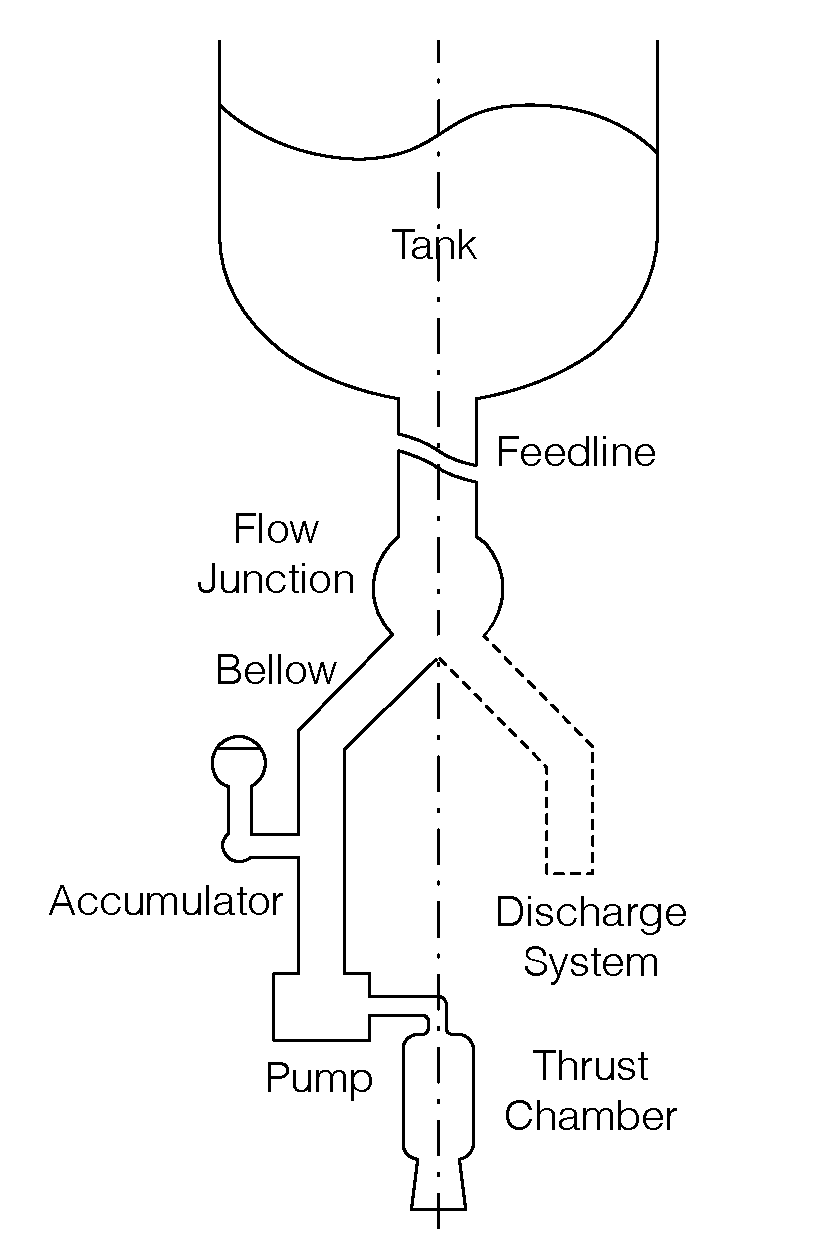
\includegraphics[width=.5\linewidth]{3D-Feedlink-Scheme}},{管路推进系统结构示意图\label{3D-Feedlink-Scheme}}]
类似节\ref{sec:Lumped-Feedline-Model},与三维推进剂贮箱对接的管路系统如图\ref{3D-Feedlink-Scheme}所示。本节沿用了之前管路元件传递函数的处理手段,首先采用有理分式拟合方法对三维贮箱对应的管路系统在形式上进行初步整理。由于液体贮箱的分析平台基于有限元分析软件MSC.Nastran,观察到其动态建模方法中提供了TF卡技术来直接修改系统整体矩阵,所以此处并没有继续采用类结构化方法处理有理分式形式的管路系统反馈力,而是利用构造TF卡的手段将其耦合到液体火箭结构系统之中。

\makebox[2\Han]{}不同于公式\eqref{eq:Feedback-Force-Transfer},由于三维贮箱不需要考虑箱底脉动流量引起反馈力,管路系统反馈力形式变为:
\protect\phantom{占座 占座 占座 占座 占座 占座 占座 占座 }

\end{figwindow}

\begin{equation}
	\label{eq:3D-Feedback-Force-Transfer}
	\boldsymbol{F}_p(s)=\left[ \begin{matrix}
	   F_2(s)  \\
	   F_3(s)  \\
	   F_4(s)  \\
	\end{matrix} \right]  \triangleq \boldsymbol{R}_{pq}(s)\left[ \begin{matrix}
	   \dot{x}_T(s)  \\
	   \dot{x}_{L1}^{(5)}(s)  \\
	\end{matrix} \right] \triangleq \boldsymbol{R}_{pq}(s)\boldsymbol{\dot{X}}_q(s)
\end{equation}

利用所得反馈力传递关系的有理分式形式,可以将公式\eqref{eq:3D-Feedback-Force-Transfer}与结构系统进行耦合:
\begin{equation}
	\left \{
	\label{eq:3D-Coupled-System-Transfer}
	\begin{aligned}
	\left[s^2 \boldsymbol{M}_s+ s\left(\boldsymbol{C}_s+\boldsymbol{\dot{M}}_s
	-\boldsymbol{L}_{sp} \boldsymbol{R}_{pq}(s)\boldsymbol{L}_{qs}\right)+ \boldsymbol{K}_s \right]\boldsymbol{X}_s(s)&=\boldsymbol{F}_s(s) \\
	s\boldsymbol{M}_{pq}+ \boldsymbol{D}_{pq}+ \sum_{k=1}^n
	\left( \frac{\boldsymbol{C}_{pq}^{(k)}}{s-\boldsymbol{A}_k} +
	\frac{\bar{\boldsymbol{C}}_{pq}^{(k)}}{s-\bar{\boldsymbol{A}}_k}  \right)
	+ \sum_{j=1}^{m}\frac{\boldsymbol{B}_{pq}^{(j)}}{s-R_j}&=\boldsymbol{R}_{pq}(s)
	\end{aligned} \right.
\end{equation}

相比集中参数管路模型,这里采用的有理分式更具通用性,考虑了传递关系中可能包含实数零点的一般情况。接下来,对于此处所得有理分式,将引入MSC.Nastran中的TF卡建模方法来对其进行进一步处理。

考察公式\eqref{eq:3D-Coupled-System-Transfer}中传递矩阵$\boldsymbol{R}_{pq}$的任一元素$R_{pq}$
\begin{equation}
	R_{pq}=T(s)=\left( sM_0 + D_0 + \sum_{k=1}^n \frac{C_k}{s-A_k}+ \sum_{k=1}^{n}\frac{\bar{C}_k}{s-\bar{A}_k} + \sum_{j=1}^{m} \frac{B_j}{s-R_j} \right) 
\end{equation}
分离实、虚部,可以使得$T(s)$中不再含有TF方法所不能处理的复数系数\footnote{由于TF卡建模方法仅支持位移传递函数的输入,而传递矩阵$\boldsymbol{R}_{pq}$表示的是速度反馈,所以在$T(s)$中分子分母同时乘以$s$以便后续处理}
\begin{equation}
	\label{eq:3D-Transfer-Single-Rational}
	T(s)=\frac{1}{s} \left[ (sM_0+D_0)s+ \sum_{k=1}^{n} \frac{2(C'_ks^2-C'_kA'_k s-C''_kA''_k s)}{s^2-2A'_ks+{A'_k}^{2}+{A''_k}^2}+\sum_{j=1}^m \frac{B_js}{s-R_j} \right]
\end{equation}
鉴于Nastran中传递函数的标准写法为($u$为节点位移):
\begin{equation}
	\label{eq:Standard-Nastran-TF}
	(B_0+B_1s+B_2s^2)u_d+\sum_i (A_{0i}+A_{1i}s+ A_{2i}s^2)u_i=0
\end{equation}
借助Epoint(辅助点)$x_1^0(t),x_{2}^k(t),x_{3}^j(t)$,其中
\begin{equation}
	\label{eq:Epoint-Relationship}
	\begin{aligned}
		X_1^0(s)&=\Laplace{x_1^0(t)}= (s^2M_0+D_0s)X_q(s) \\
		X_{2}^k(s)&=\Laplace{x_2^k(t)}= X_q(s)/(s^2-2A'_ks+{A'_k}^2+{A''_k}^2)\\
		X_{3}^j(s)&=\Laplace{x_3^j(t)}= X_q(s)/(s-R_j)
	\end{aligned}
\end{equation}
可以利用公式\eqref{eq:3D-Transfer-Single-Rational}写出传递矩阵$T(s)$对于反馈力$\boldsymbol{F}_p(s)$的贡献:
\begin{equation}
	\label{eq:Quasi-Structural-Epoint}
	\begin{aligned}
		f^{q}(s)&= T(s)\dot{X}_q(s) =X_1^0(s) + \sum_{j=1}^m (B_js)X_3^{j}(s) \\
		&+\sum_{k=1}^n 2(C'_k s^2- C'_k A'_k s- C''_k A''_ks)X_2^{k}(s)
	\end{aligned}
\end{equation}
考虑到传递矩阵$\boldsymbol{R}_{pq}$中各个分量的极点是相同的,为了尽可能少的引入Epoint,在对其整体进行TF卡片输入的时候,辅助点$\tilde{\boldsymbol{X}}(s)$的引入规范如下:
\begin{equation}
	\label{eq:General-Epoint-Relationship}
	\begin{aligned}
		{\tilde{X}}_{pq}^{(0)}(s)&=(s^2M_{pq}+D_{pq}s)X_q(s) \\
		{\tilde{X}}_{q}^{(k)}(s)&=X_q(s)/(s^2-2A'_ks+{A'_k}^2+{A''_k}^2)\\
		{\tilde{X}}_{q}^{(j)}(s)&=X_q(s)/(s-R_j)
	\end{aligned}
\end{equation}
可知辅助点的总数目为$p\cdot q+ q\cdot k+ q\cdot j$。TF卡片的示例样式如图\ref{TF-Card-Construction}。

\begin{figure}[!htb]
  \centering
  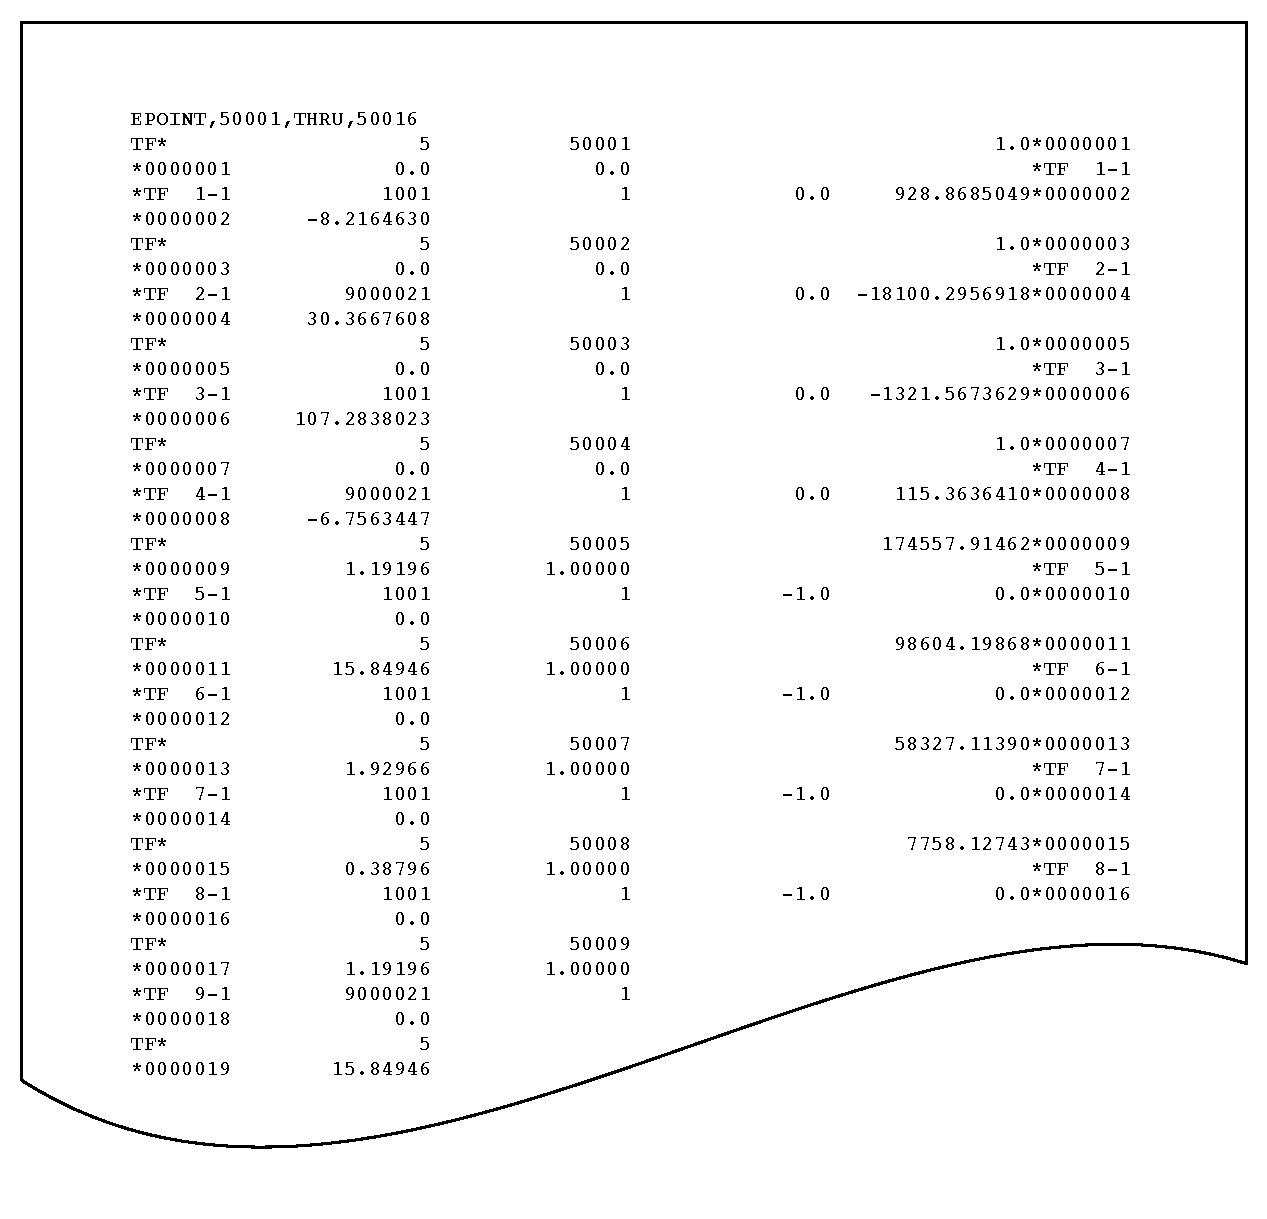
\includegraphics[width=\linewidth]{TF-Card-Construction}
  \caption{MSC.Nastran传递函数TF卡片构造示例}\label{TF-Card-Construction}
\end{figure}

最后,可利用公式\eqref{eq:General-Epoint-Relationship},写出传递矩阵$\boldsymbol{R}_{pq}$中任意元素$R_{pq}$对于反馈力$\boldsymbol{F}_p(s)$的贡献:
\begin{equation}
	\label{eq:General-Quasi-Structural-Epoint}
	\begin{aligned}
		f_{pq}(s)&= R_{pq}\dot{X}_q(s)={\tilde{X}}_{pq}^{(0)}(s) + 
		\sum_{j=1}^m (B_{pq}^{(j)}s){\tilde{X}}_{q}^{(j)}(s) \\
		&+\sum_{k=1}^n 2(C_{pq}^{\prime (k)} s^2- C_{pq}^{\prime (k)} A'_k s- C_{pq}^{\prime\prime(k)} A''_ks){\tilde{X}}_{q}^{(k)}(s)
	\end{aligned}
\end{equation}
观察公式\eqref{eq:General-Epoint-Relationship}和\eqref{eq:General-Quasi-Structural-Epoint},可见其均满足Nastran的输入要求\eqref{eq:Standard-Nastran-TF}。于是,方程\eqref{eq:3D-Coupled-System-Transfer}最终可以被划归为二阶常微分方程组的传递矩阵形式:
\begin{equation}
	\label{eq:3D-Final-Coupled-Transfer-Function}
	(s^2\boldsymbol{M}_c+s\boldsymbol{C}_c+\boldsymbol{K}_c)\boldsymbol{X}_c(s)=\boldsymbol{F}_c(s)
\end{equation}
其中,$\boldsymbol{X}_c(s)=\left[ \boldsymbol{X}_s^{\ut}(s)\quad \tilde{\boldsymbol{X}}^\ut(s) \right]^{\ut}$为包含辅助点自由度的增广节点位移向量,$\boldsymbol{M}_c,\boldsymbol{C}_c,\boldsymbol{K}_c$为重新装配后的耦合系统质量、阻尼和刚度矩阵。可以看到,由于辅助变量的引进,耦合系统整体矩阵不再保持原有的对称性,所以通常需要利用成熟的复模态求解方法对其进行复特征值和特征向量的求解。不过,相对于求解管路系统原始的非线性反馈力传递矩阵而言,Nastran等商业有限元软件的计算效率和求解精度都要远远胜出。

\section{耦合系统阻尼特性分析}
随着充液航天器的发展,带液贮箱的阻尼特性分析正引起越来越多研究者的关注。然而,由于人们对于物质在其运动过程中能量耗散的成因及机理分析还很不完善,以至于就单纯的结构或者流体动力学问题而言,系统阻尼的建模、校核与评估通常即为求解问题中最难处理的一部分。对于POGO振动问题,由于液体火箭的结构阻尼一般是由实验测定得出,所以此处本节着重介绍了贮箱内部液体的阻尼计算。

\subsection{液体阻尼特性分析基础}
在节\ref{sec:Three-Dimensional-Tank-Model}介绍的带液贮箱建模过程中,由于本文的研究重点为液体火箭的纵向耦合振动,所以模型并没有考虑贮箱内部液体晃动等与耦合系统纵向振动联系较弱的其他运动形式。然而,针对贮箱内部液体的阻尼建模问题,因为液体阻尼主要与箱体壁面粘性阻尼作用、自由液面处的粘性耗散、液体内部粘性耗散及毛细作用等四个方面相关联\cite{Henderson:1994, Martel:1998},所以此时必须将贮箱内液体的晃动等方面考虑进来。

该方法认为理想流体区域的运动由Laplace方程控制($\Phi$为速度势):
\begin{equation}
	\label{eq:Ideal-Liquid-Laplace}
	\left \{
	\begin{alignedat}{2}
	&\nabla^2\Phi=0 &\quad &\text{液体内部}\:\Omega\\
	&{\displaystyle \frac{\partial \Phi}{\partial n}}=0 &\quad &\text{不可渗透边界条件}\:S_w \\
	&{\displaystyle \frac{\partial \Phi}{\partial t}}=-gh  &\quad &\text{液体自由面}\:S_f
	\end{alignedat} \right.
\end{equation}
对于Stokes边界层,由于其厚度在一般情况下非常薄,因此可以将壁面边界层内某一点的流动速度近似处理为于壁面平行:
\begin{equation}
	\frac{\partial \boldsymbol{v}}{\partial t} = \nu\frac{\partial^2 \boldsymbol{v}}{\partial z^2}
\end{equation}
其中$\boldsymbol{v}$为流体速度,$z$为壁面法向坐标,$\nu$为液体的运动学粘度系数。根据计算所得的流体运动情况,就可以计算Stokes边界层与流体内部粘性的能量耗散。

\begin{enumerate}[label=\textbf{\Roman*.}, align=left, leftmargin=0pt, listparindent=\parindent, itemindent=!, labelwidth=\parindent, labelsep=0pt, itemsep=1em]
\litem{Stokes边界层能量耗散}
\begin{itemize}
\item 对于液面没有受到污染的情况:仅在壁面上计算Stokes边界层。若假设$\boldsymbol{v}=\boldsymbol{U}e^{i\omega t}$,一个晃动周期内的平均能量耗散率为
\begin{equation}
	D_1=\rho\sqrt{\frac{1}{8}\nu\omega}\iint_{S_w}| \boldsymbol{U}|^2\ud S
\end{equation}
\item 对于自由液面受到污染的情况:需要额外考虑自由液面处的Stokes边界层能量耗散
\begin{equation}
	D_1=\rho\sqrt{\frac{1}{8}\nu\omega}\iint_{S_w+S_f}| \boldsymbol{U}|^2\ud S
\end{equation}
\end{itemize}

\litem{流体内部的能量耗散}
\begin{itemize}
\item[]对于流体的粘性耗散有如下耗散函数:
\begin{equation}
	F=\frac{\mu}{2}\int_{\Omega}\mathfrak{R}(\boldsymbol{v})\ud\Omega
\end{equation}
其中$\mu$为动力学粘度系数,$\boldsymbol{v}=\left[ \begin{matrix} v_x & v_y & v_z \end{matrix} \right]^\ut$
\begin{displaymath}
	\begin{aligned}
		\mathfrak{R}(\boldsymbol{v})=&2\left[(\frac{\partial v_x}{\partial x})^2 + (\frac{\partial v_y}{\partial y})^2+ (\frac{\partial v_z}{\partial z})^2\right] \\
		&+ (\frac{\partial v_z}{\partial y}- \frac{\partial v_y}{\partial z})^2+(\frac{\partial v_x}{\partial z}- \frac{\partial v_z}{\partial x})^2 + (\frac{\partial v_y}{\partial x}- \frac{\partial v_x}{\partial y})^2
	\end{aligned}
\end{displaymath}
利用方程\eqref{eq:Ideal-Liquid-Laplace},可以写出一个周期内液体内部的平均能量耗散率为:
\begin{equation}
	\begin{aligned}
		D_2&=\frac{\omega}{2\pi}\int_0^{\frac{2\pi}{\omega}}2F(\Phi)\ud t \\
		&=\frac{\omega}{2\pi}\int_0^{\frac{2\pi}{\omega}}\mu\int_\Omega \mathfrak{R}(\Phi)\ud \Omega \cos ^2 (\omega t)\ud t \\
		&=\frac{1}{2}\mu\int_\Omega\mathfrak{R}(\Phi)\ud \Omega
	\end{aligned}
\end{equation}
\end{itemize}
\end{enumerate}
如此,由于在一个周期内液体晃动的总机械能为
\begin{equation}
	E=\frac{\rho}{2}\int_\Omega |\nabla \Phi|^2\ud \Omega
\end{equation}
可以计算出贮箱内液体阻尼比$\gamma$为\cite{Abramson:1966, Miles:1958}:
\begin{equation}
	\label{eq:Damping-Ratio-Stokes}
	\gamma=\frac{D_1+D_2}{2\omega E}
\end{equation}
实际上,Abramson早在1966年便通过实验数据的拟合,给出了圆柱容器内液体小幅晃动第一阶模态阻尼的经验公式\cite{Abramson:1966}:
\begin{equation}
	\label{eq:Empirical-Damping-Ratio}
	\delta=4.98\nu^{1/2}R^{-3/4}g^{-1/4}\left[ 1+\frac{0.318}{\sinh (1.84{\displaystyle\frac{h}{R}})} \left( \frac{1-{\displaystyle\frac{h}{R}}}{\cosh(1.84{\displaystyle\frac{h}{R}})} +1\right) \right]
\end{equation}
其中$R$为容器的半径,$h$为容器内部液体高度,$g$为当地重力加速度。经过验证,在$\displaystyle \frac{h}{R}<1.0$的时候,公式\eqref{eq:Damping-Ratio-Stokes}与\eqref{eq:Empirical-Damping-Ratio}给出的计算结果相当一致\cite{WangWei:2005,WangWei:2006}。但是,由于上述Henderson模型建立在线性化自由表面边界的基础之上,所以其结论仅局限在液面做小幅晃动的时候。对于$\displaystyle \frac{h}{R}>1.0$的情况,Abramson给出了另外的经验公式:
\begin{equation}
	\delta=4.98\nu^{1/2}R^{-3/4}g^{-1/4}
\end{equation}
由此可见,现阶段可以通过理论推导来获得的阻尼模型还很有限,计算模型的验证还远远离不开实验去验证。

\subsection{带防晃板的贮箱液体阻尼}
Mikishev和Stephens等人经过大量的科学实验,发现液体的粘性耗散作用其实在防止液体晃动方面真正能起到的作用非常有限\cite{Mikishev:1961, Stephens:1962}。在正常规格的贮箱内部,即使内部装有动力学粘度超出水一百倍的液体,其粘性阻尼也不会超过0.5\si{\percent}。因而,对于液体火箭这种需要严格控制液体晃动的复杂构型,Baffle(防晃板)的使用是必不可少的。

存在防晃板的液体建模其实与公式\eqref{eq:Ideal-Liquid-Laplace}非常类似,获得解析解的技术手段一般也即为时间-空间分离变量法。若在贮箱根部建立$rz\theta$柱坐标系,假设贮箱底部存在$\ddot{x}(t)=\ddot{x}_0e^{\num{i}\omega t}$的简谐运动,那么可以构造公式\eqref{eq:Ideal-Liquid-Laplace}速度势函数解析解的对流部分\cite{Haroun:1981}:
\begin{gather}
	\Phi_c=\left( \frac{g\eta}{\num{i} \omega} \right)\frac{\cosh(\lambda_1 z/R)}{\cosh(\lambda_1 H/R)} \\
	\eta(r,\theta,t)=R\left[ \sum_{j=1}^\infty \frac{1}{1-{(\omega/\omega_j)}^2} \frac{2}{\lambda_j^2-1} \frac{J_1(\lambda_j r/R)}{J_1(\lambda_j)} \right]\frac{\ddot{x}_0}{g}e^{\num{i}\omega t} \cos\theta \nonumber
\end{gather}

其中,$R$为贮箱半径,$H$为液面总高度,$\eta$为液面晃动振幅。$J_1$为第一类Bessel函数,$\lambda_j$为$\dot{J}_1$的第$j$个零点,$\omega_j$为液体晃动的第$j$阶固有频率。
\begin{displaymath}
	{\omega_j}^2=\frac{\lambda_j g}{R}\tanh \left( \lambda_j \frac{H}{R} \right)
\end{displaymath}
Stricklin经过计算得出了晃动液体的总机械能为\cite{Stricklin:1966}:
\begin{equation}
	E=\frac{1}{4} \rho g \eta^2 \left( 1- \frac{1}{\lambda_1^2} \right)\pi R^2
\end{equation}
对于存在防晃板情况下液体的能量损耗,可以通过衡量板内微元$\ud A$面积下的阻力$\ud F$,对其积分来计算防晃板的平均做功:
\begin{align}
	\ud F&=\frac{1}{2}\rho C_d u_n|u_n|\ud A \\
	D&=\overline{\int u_n \ud F}
\end{align}
其中$u_n=u_n(r,\theta,z,t)$是液体沿防晃板法线方向的运动速度,$C_d$为阻力系数。将阻力做功在一个晃动周期内进行平均,可以获得贮箱液体的平均能量损耗:
\begin{equation}
	\label{eq:Baffle-Energy-Loss}
	D=\int\frac{2}{3\pi}\rho C_dU_n^3 \ud A
\end{equation}
可以看出,方程\eqref{eq:Baffle-Energy-Loss}计算的关键在于确定阻力系数$C_d$与液体晃动速度$U_n$。然而,对于不同的液体及防晃板类型,$C_d$通常只能利用实验手段获得。以环形防晃板为例,Keulegan和Carpenter给出了$C_d$的拟合公式\cite{Keulegan:1958}:
\begin{equation}
	\label{eq:Ring-Baffle-Cd}
	C_d=15 \left( \frac{UT}{r_b} \right)^{-0.5},\quad 2\leq \frac{UT}{r_b} \leq 20
\end{equation}
其中$T$为液体晃动周期,$r_b$为防晃板宽度,$U$为垂直防晃板方向的液体流动速度。将公式\eqref{eq:Baffle-Energy-Loss}及\eqref{eq:Ring-Baffle-Cd}带入\eqref{eq:Damping-Ratio-Stokes},Maleki给出了环形防晃板的阻尼比计算公式\cite{Maleki:2008}:
\begin{equation}
	\label{eq:Ring-Baffle-Damping-Ratio}
	\gamma_r=4C_r \sqrt{\frac{\eta_m}{R}} \left( \frac{\sinh (1.84h/R)}{\sinh (1.84H/R)} \right)^{2.5} \tanh \left( 1.84\frac{H}{R} \right)
\end{equation}
其中$h$为防晃板安装高度,$\eta_m$为最大液面晃动幅度。$C_r$与防晃板相对面积有关:
\begin{equation}
	C_r=\left(\frac{r_b}{R}\right)^{1.5} \left(2- \frac{r_b}{R}\right) 
\end{equation}

\begin{figure}[!htb]
  \centering
  \includegraphics[width=\linewidth]{Ring-Baffle-Damping-Curve.pdf}
  \caption{有环形防晃板的贮箱液体阻尼}\label{Ring-Baffle-Damping-Curve}
\end{figure}

值得注意的是,由公式\eqref{eq:Ring-Baffle-Damping-Ratio}与Maleki的贮箱实验结果可以看出:液体阻尼将随液面高度$H/R$变化而变化;对于液体火箭来说,推进剂贮箱半满状态时的液体阻尼要远高于其满箱和空箱状态(如图\ref{Ring-Baffle-Damping-Curve}\cite{Maleki:2008},$\eta/R=0.05,\, r_b/R=0.2$)。此外,对于没有防晃板的情况而言,公式\eqref{eq:Empirical-Damping-Ratio}给出的计算结果不仅阻尼很小,并且没有体现这种变化趋势。这就要求POGO研究者们在对液体火箭带液贮箱进行建模分析的时候,必须格外关注以下几点:
\begin{enumerate}
	\item 严格区分不同类型贮箱的液体阻尼计算模型;
	\item 具备实验条件的情况下,尽可能开展带液贮箱的振动实验以验证计算结果的准确性;
	\item 必须考虑液体贮箱阻尼特性的时变规律。
\end{enumerate}

此外,随着近年来流体力学计算方法的发展,一些学者也开始尝试通过有限体积法的VOF方法对贮箱液体进行了更为精细的动态仿真。例如,杨魏等针对圆柱箱体中的液体晃动阻尼开展了数值仿真\cite{YangWei:2009},虽然其模型中应用的防晃板并非环形,但是贮箱内部液体的阻尼变化规律大致与Maleki模型相同(如图\ref{YangWei-Baffle},\ref{Damping-Ration-Yang})。鉴于液体火箭真实模型的贮箱实测非常难以实施,以上方法也为带液贮箱的阻尼特性分析提供了新的思路。

\begin{figure}[!htb]
\hspace{\stretch{2}}
\begin{minipage}[b]{0.35\textwidth}
  \centering
  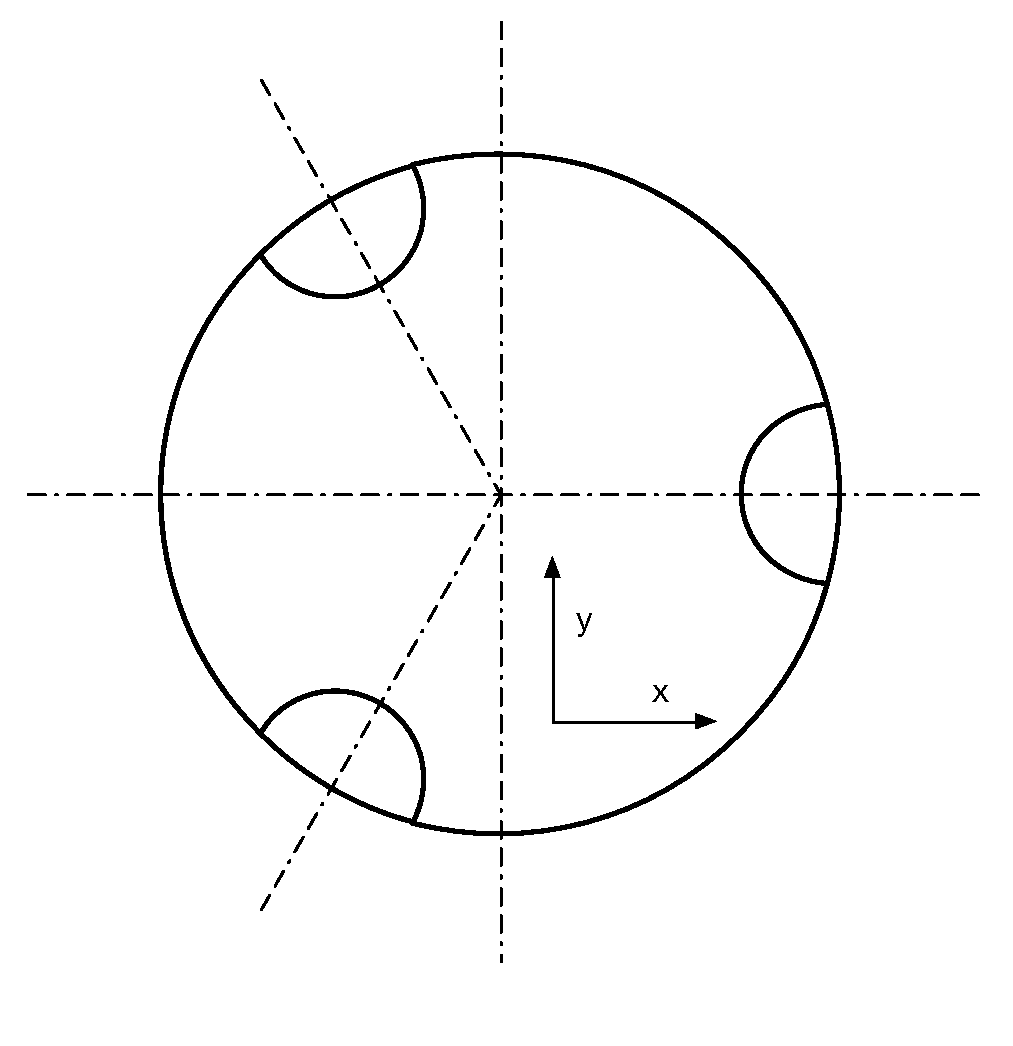
\includegraphics[width=\linewidth]{Baffle}
  \caption{半圆形防晃板配置图}\label{YangWei-Baffle}
\end{minipage}
\hspace{\stretch{1}}
\begin{minipage}[b]{0.55\textwidth}
  \centering
  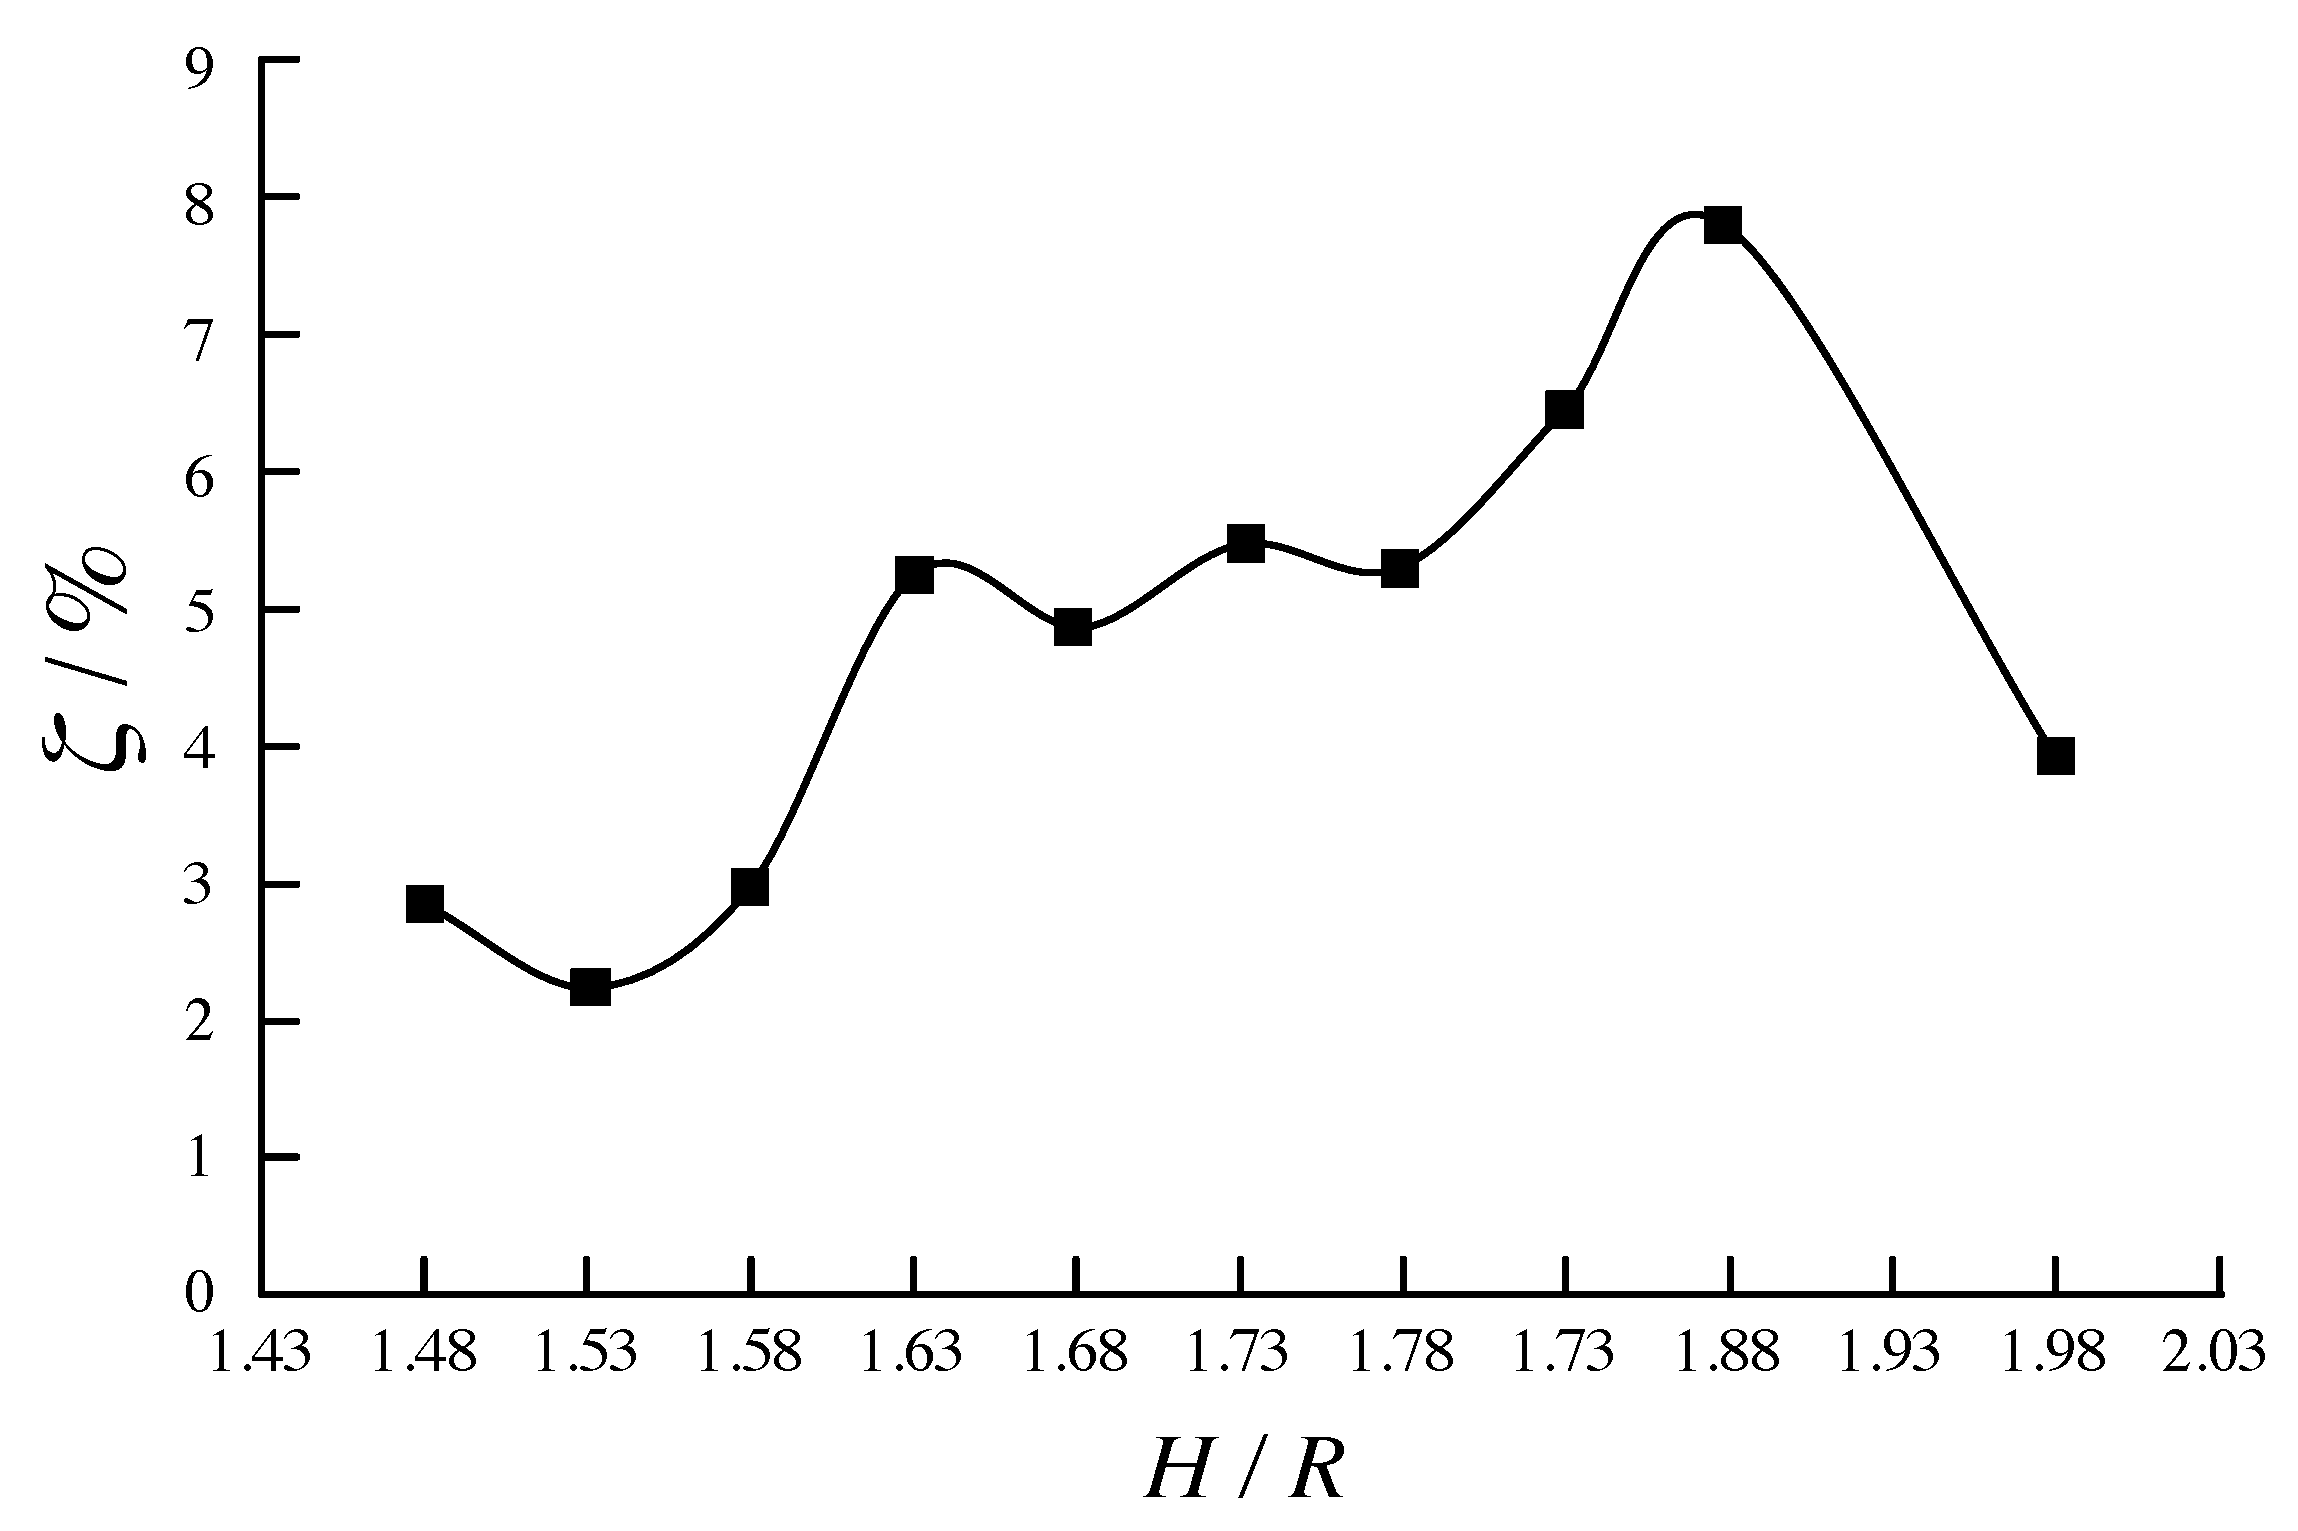
\includegraphics[width=\linewidth]{Damping-Ration-Yang}
  \caption{不同液面高度晃动阻尼比计算结果}\label{Damping-Ration-Yang}
\end{minipage}
\end{figure}

\subsection{贮箱液体阻尼的应用方法}
综合前两节的结论,可以看出耦合系统阻尼特性分析的重点和难点主要在于:
\begin{enumerate}[leftmargin=\parindent, align=parleft, labelindent=0pt, labelwidth=*]
\item 如何根据已有的带液贮箱实验数据及防晃板参数来确定阻力系数$C_d$,进而推导得出贮箱液体的阻尼比时变参数;
\item 如何将贮箱液体的阻尼特性包含于三维贮箱的建模之中,进而参与耦合系统动力学计算。
\end{enumerate}
由于前者的解决方法主要依赖现有实验手段而非进一步的理论推导,所以本节主要介绍如何在有限元方法中实现对于带液贮箱时变阻尼特性的建模分析。

在系统动力学中,阻尼通常可以分为粘性阻尼和结构阻尼两种,其数学描述如下:
\begin{equation}
	\begin{cases}
	f_v=b\dot{u} & \text{粘性阻尼力}\\
	f_s=\num{i}gku & \text{结构阻尼力} \\
	\end{cases}
\end{equation}
其中$\num{i}=\sqrt{-1}$,$b$为粘性阻尼系数,$g$为结构阻尼系数,$k$为结构刚度。可以看出,对于系统复模态分析来说,粘性阻尼力不仅与粘性阻尼系数相关,并且与外界扰动力频率$\omega$成正比。所以,若想通过调节阻尼系数来将两种阻尼模型等效互换,通常只能在特定频段之内操作:
\begin{equation}
	gk=b\omega\ \longrightarrow\ b=\frac{gk}{\omega}
\end{equation}
若外界扰动力频率$\omega$恰好等于系统固有频率,则
\begin{gather}
	\omega=\omega_n=\sqrt{\frac{k}{m}} \\
	b=\frac{gk}{\omega_n}=g\omega_n m
\end{gather}
由于系统的临界阻尼满足$b_c=2m\omega_n$,可以推导得出在共振点附近结构阻尼比$\zeta$满足:
\begin{equation}
	\label{eq:G-B-Zeta}
	\frac{b}{b_c}=\zeta=\frac{g}{2}
\end{equation}
假如已经通过实验等方法成功获取了带液贮箱的阻尼参数,可以根据公式\eqref{eq:G-B-Zeta}进行不同阻尼系数之间的换算。

系统复模态的计算方法通常可以分为两种:直接法和模态法。由于POGO振动的快速特征值求解法并没有采用模态缩聚技术,所以此处主要介绍如何针对直接法进行结构系统阻尼和贮箱液体阻尼的施加。

以MSC.Nastran为例,其阻尼输入方法可以分为两大类:直接矩阵输入法与参数设定法。
\begin{enumerate}[leftmargin=\parindent, align=parleft, labelindent=0pt, labelwidth=*]
\item 假如用户已经通过外部计算获得了系统阻尼矩阵,可以利用直接矩阵输入法将计算结果导入求解器(对称矩阵B2GG,对称或不对称矩阵B2PP);
\item 参数设定法则是通过指定模型中相关材料的结构阻尼系数$G_e$,或是直接设定系统整体的结构阻尼系数$G$或Rayleigh阻尼系数$\alpha_1,\alpha_2$\footnote{修改后的系统阻尼矩阵$\boldsymbol{B}'= \boldsymbol{B}+\alpha_1\boldsymbol{M}+\alpha_2\boldsymbol{K}$}来实现仿真对象的阻尼特性建模。
\end{enumerate}

\begin{figure}[!tb]
  \centering
  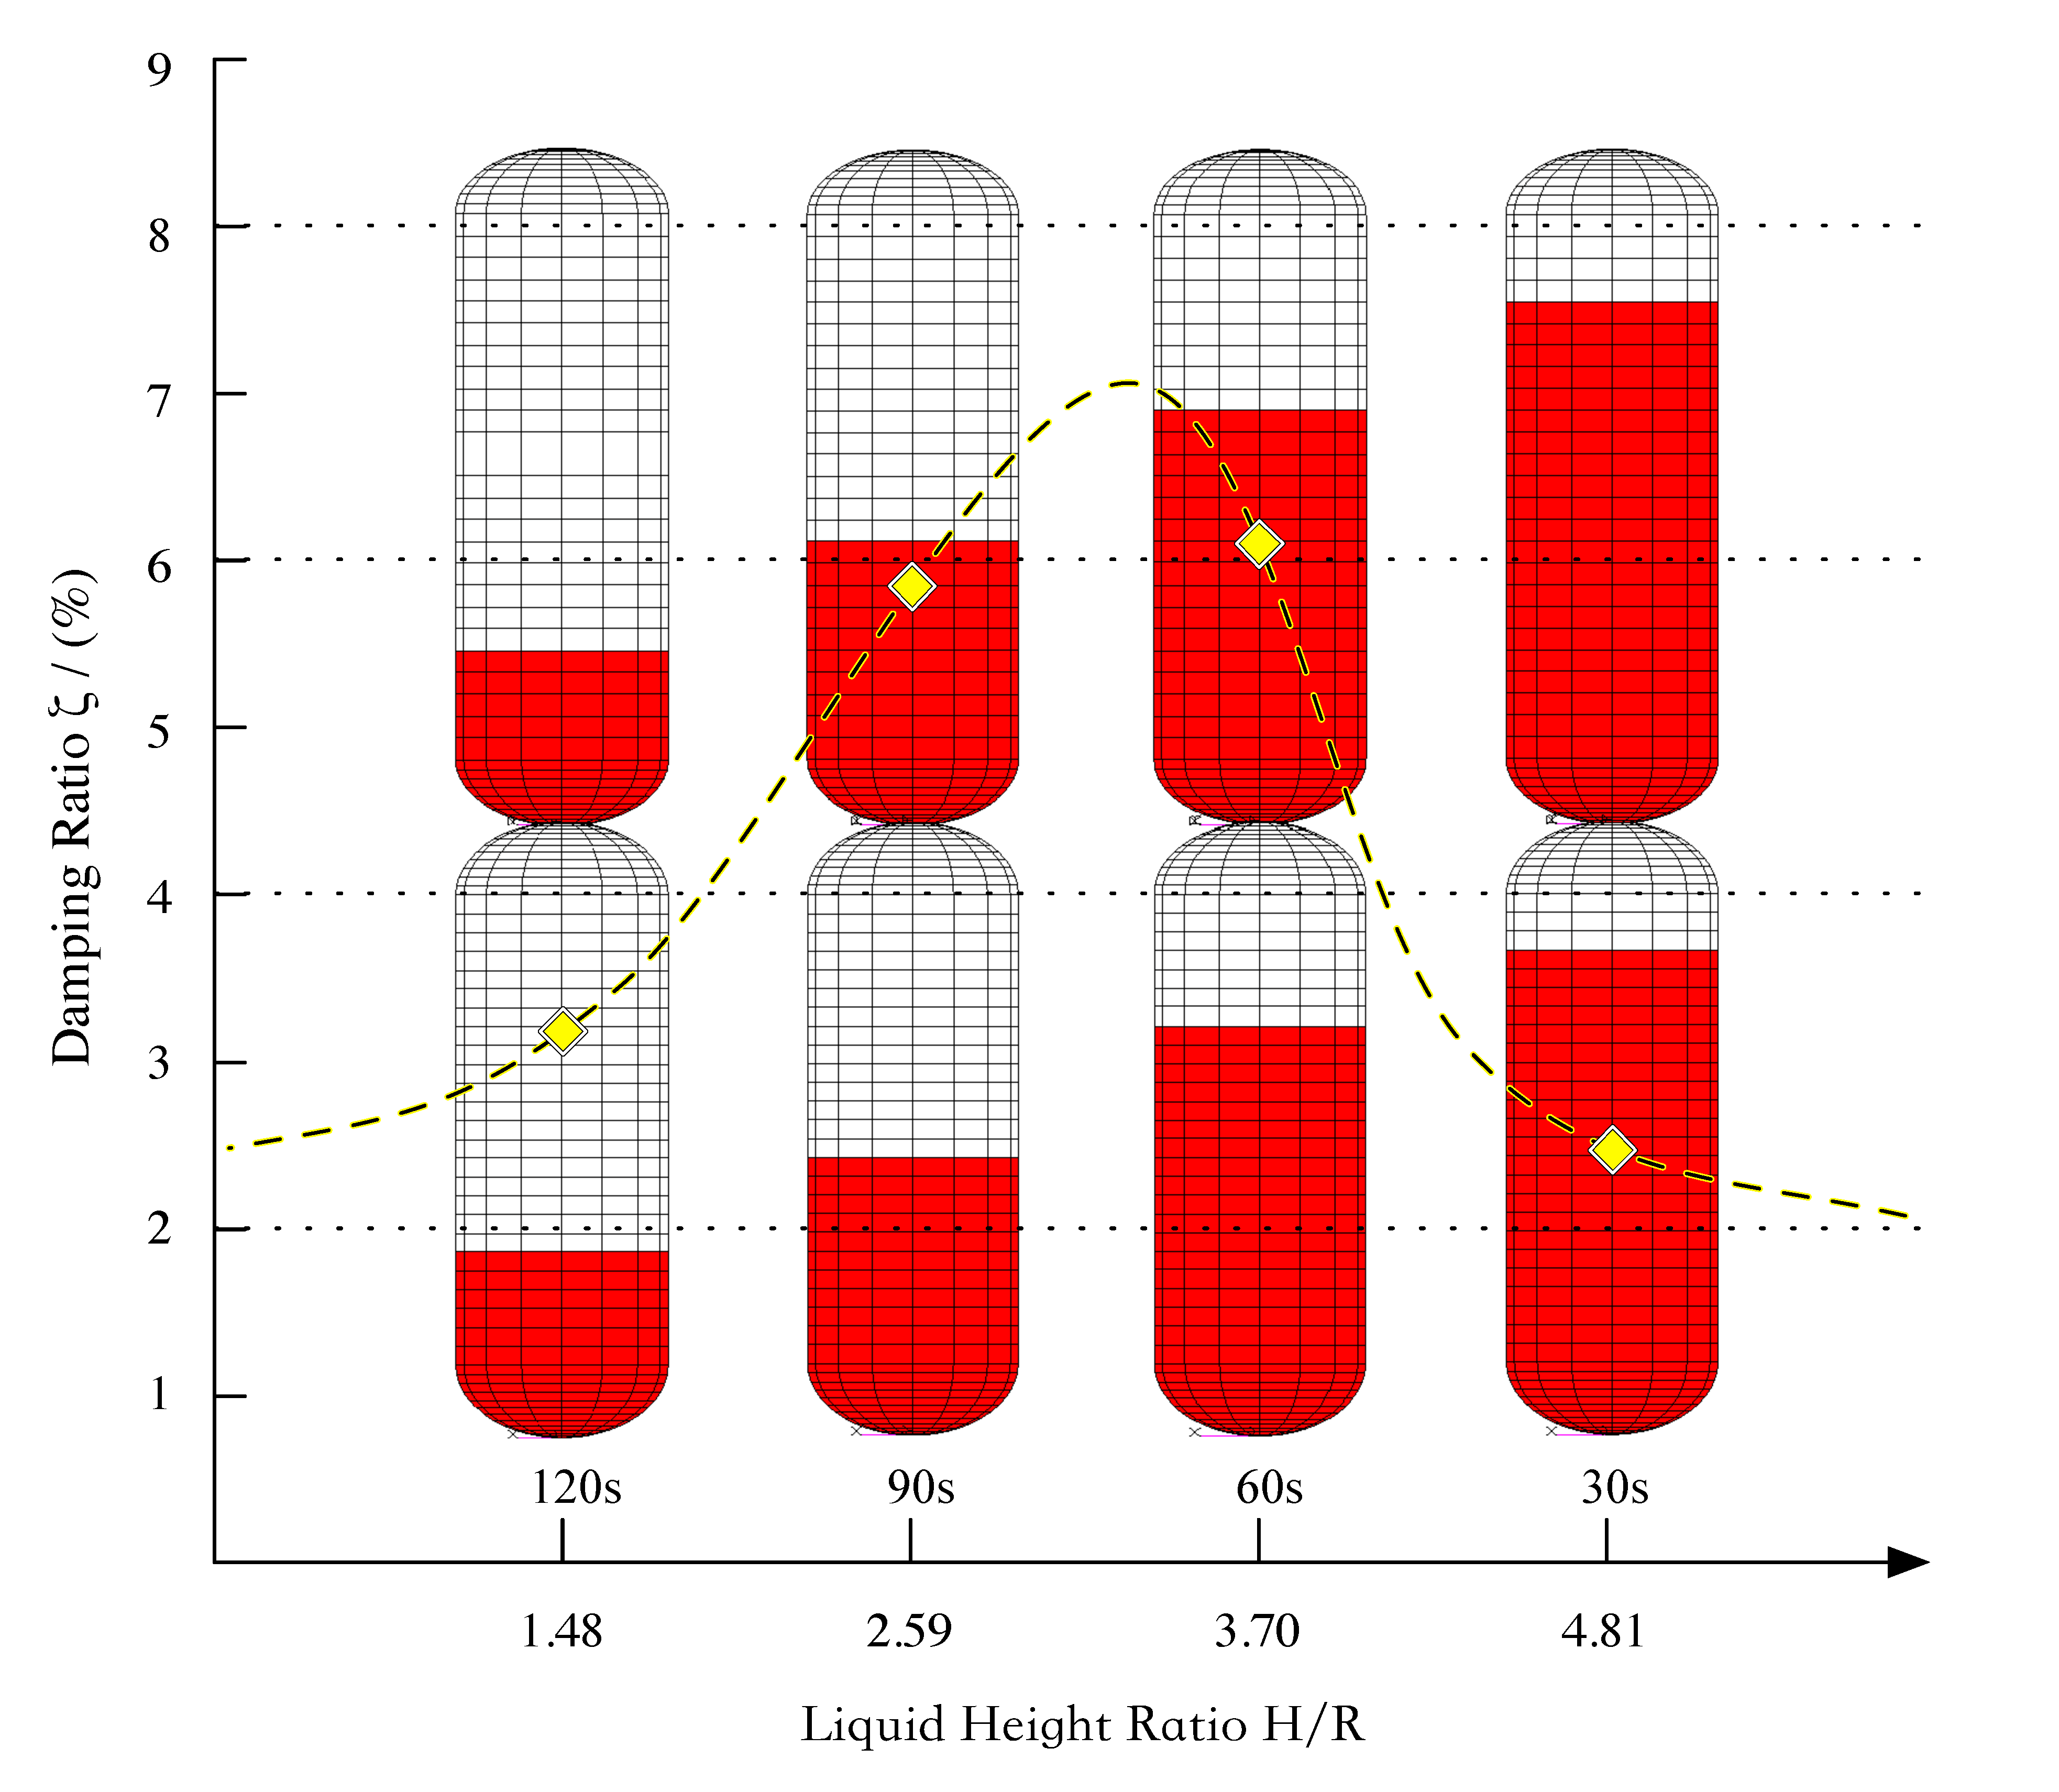
\includegraphics[width=\linewidth]{Time-Varing-Tank-Height}
  \caption{三维贮箱液体阻尼随高度变化示意图}\label{Time-Varing-Tank-Height}
\end{figure}

\section{算例分析}
参考节\ref{sec:Lumped-Numerical-Simulation}中算例,为了与其进行对比,本节采用同样的准静态技术与管路系统模型参数对相同规格的国内某液体火箭开展了耦合系统稳定性分析。不同的是,本例在对液体火箭结构系统建模时引入了节\ref{sec:3D-Liquid-Tank-Modelling}中介绍的带液贮箱三维模型,同时还利用节\ref{sec:3D-Tank-VS-Feedline-Update}中描述的TF卡建模方法对与其配套的管路系统进行对接处理。

\begin{figure}[p]
  \centering
  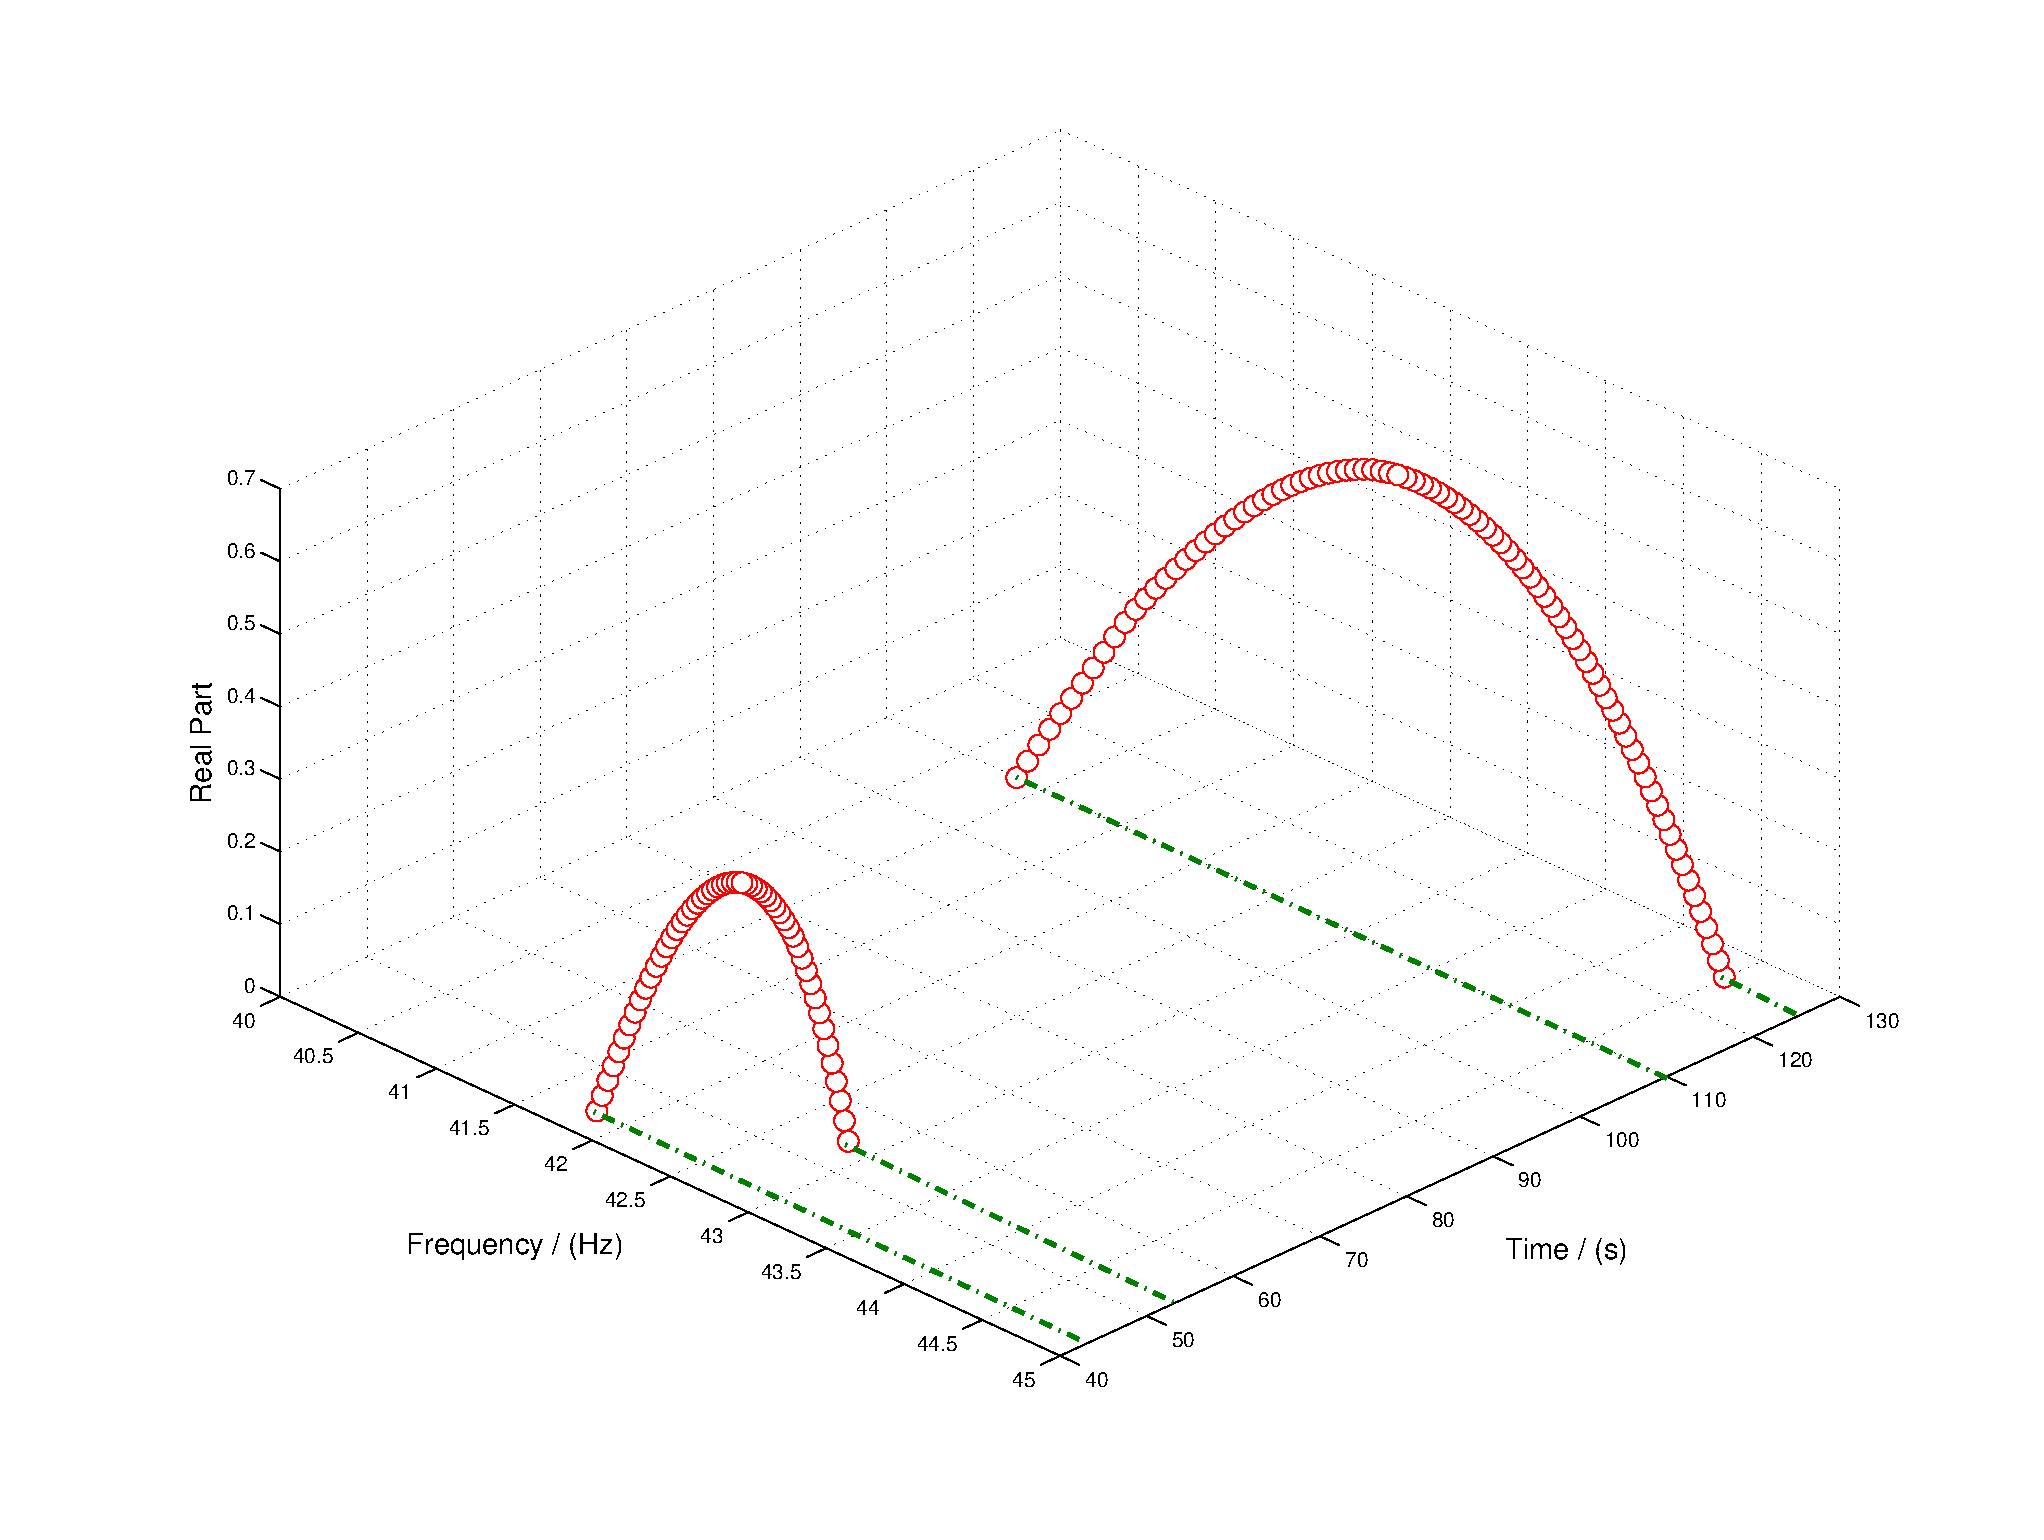
\includegraphics[width=\linewidth]{3D-Stability-Curve}
  \caption{耦合系统特征值随时间变化三维曲线}\label{3D-Stability-Curve}
  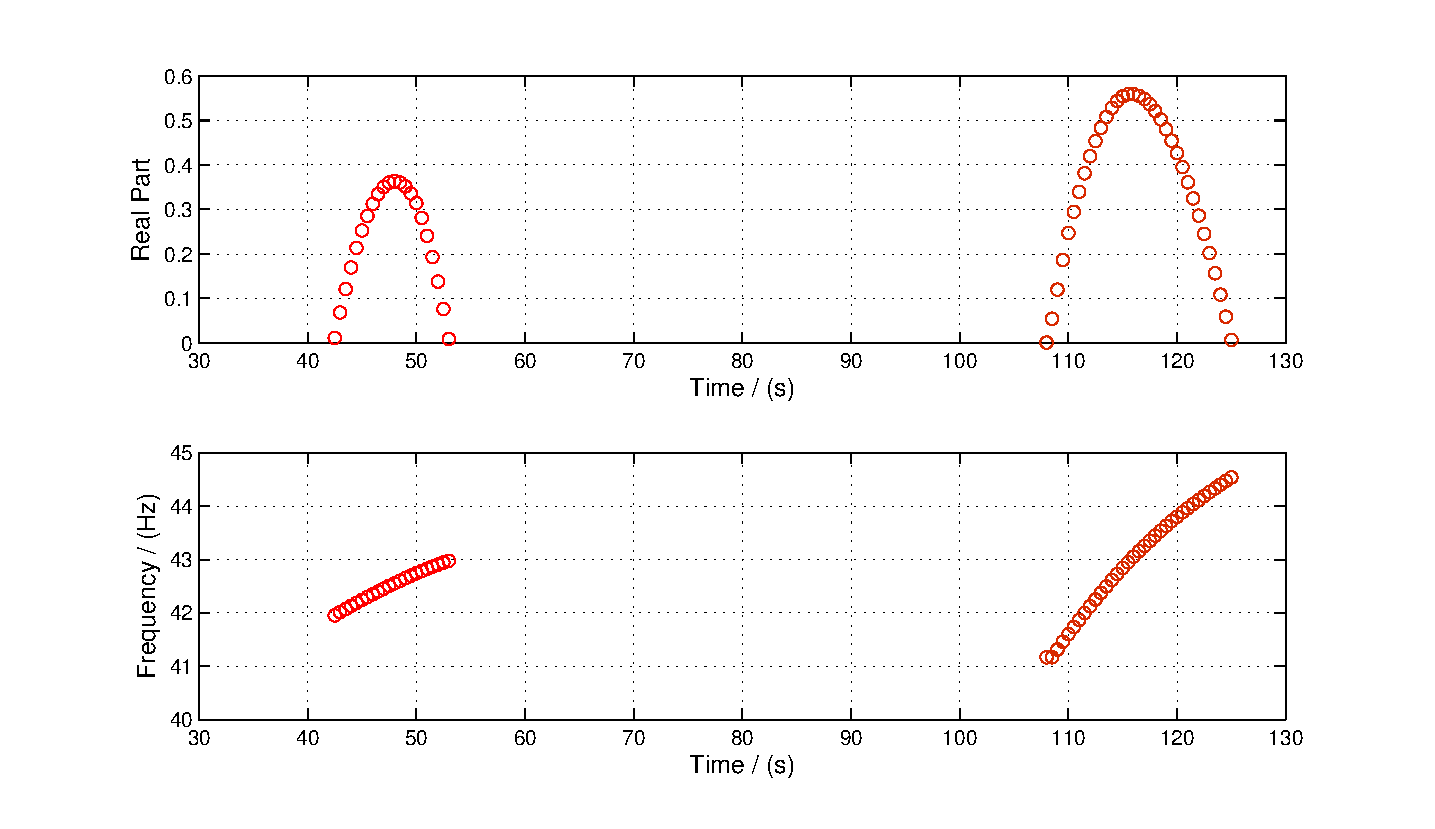
\includegraphics[width=\linewidth]{3D-Stability-Real-Imag}
  \caption{耦合系统特征值三维曲线的正视图与俯视图}\label{3D-Stability-Real-Imag}
\end{figure}

首先,图\ref{3D-Stability-Curve}给出了耦合系统特征值随时间变化三维曲线。由于POGO稳定性分析关注的主要为系统特征值是否包含正实部,所以图中仅显示了特征值包含正实部的部分结果。可以清晰的看出,相比与节\ref{sec:Lumped-Numerical-Simulation}中阐述的液体火箭为全时稳定的结论,该曲线表明此火箭在升空过程中经历了两个包含不稳定振动的时间区段。结合图\ref{3D-Stability-Real-Imag}给出的三维曲线正视图和俯视图,可以发现这两次不稳定振动存在以下特征:
\begin{enumerate}
	\item 不稳定模态的固有频率都随着时间从低到高变化;
	\item 不稳定模态的正实部时间演化都呈现抛物线形;
	\item 第二次失稳的时间历程与对应特征值的正实部较第一次来说更长、更大。
\end{enumerate}

从上述不稳定振动的特征描述来看,这两次失稳都基本符合POGO振动的主要特征。由于两次失稳的固有频率明显没有延续性,这就意味着该液体火箭不仅在运行期间发生了多次POGO振动,并且每次被激发的耦合系统模态可能不尽相同。

\setcounter{footnote}{0}

\begin{figure}[p]
  \centering
  \includegraphics[width=\linewidth]{50s-Modal-Deformed.png}
  \caption{液体火箭带有正实部的贮箱局部模态剖面图:50s时刻}\label{50s-Modal-Deformed}
  \vspace{1.5em}
  \includegraphics[width=\linewidth]{120s-Modal-Deformed.png}
  \caption{液体火箭带有正实部的贮箱局部模态剖面图:120s时刻}\label{120s-Modal-Deformed}
  \vspace{1.5em}
  \includegraphics[width=\linewidth]{Deformed-Modal.pdf}
  \caption{液体火箭带有正实部的复模态局部振型:50s时刻}\label{Deformed-Modal}
\end{figure}

为了揭示POGO振动所处模态与其他正阻尼模态有何差异,图\ref{3D-Modal-Bottom}给出了两组耦合系统失稳模态与其相邻模态之间的局部振型形貌对比\footnote{各阶模态均采用统一的归一化方法}。通过观察氧化剂贮箱箱底及发动机燃烧室处的振动情况,可以发现:
\begin{itemize}
	\item[-] 由于推进剂贮箱壳体的柔度普遍高于液体火箭结构系统其他部位,所以耦合系统正阻尼模态通常也会展现出贮箱底部变形较大的情况;
	\item[-] 考虑到发动机燃烧室处的节点在质量和连接刚度上并无异于其他集中参数质量节点,所以其振动量级一般不会显著高于液体火箭其他部位。因此,在进行耦合系统复模态分析时,要特别关注在燃烧室处存在振动异常的高危振型---只有在发生POGO振动时,此处才有可能由于管路系统反馈力的影响而产生振幅剧烈放大的异常现象。
\end{itemize}









%\include{Chapter03}

%% !TEX encoding = UTF-8 Unicode
%!TEX TS-program = xelatex

\chapter{结论与展望}

\section{全文总结}
乘着祖国大力发展载人航天事业的契机,本文以液体火箭纵向耦合振动的稳定性分析为主要研究内容,比较深入的阐述了POGO问题的研究对象、作用机理、求解方法及预防手段。全文研究工作的要点及创新点主要包括:
\begin{enumerate}[leftmargin=0pt, align=parleft, itemindent=2\parindent, labelsep=0pt, label=\roman*).]
	\item 较为全面的总结了国内、外液体火箭纵向耦合问题的研究进展,指出了传统的液体火箭POGO稳定性分析方法如矩阵法、单传法和临界阻尼法,在求解非对称、非线性复传递矩阵特征值时遇到的主要问题及方法局限性。
	\item 发展了一种基于矩阵法和有理分式拟合法的耦合系统快速特征值求解算法。该方法能够利用类结构化建模技术将包含超越函数的管路推进系统反馈力传递函数等效变换为与结构动力学方程一致的形式,通过求解矩阵特征值问题以快速、精确的确定耦合系统动力学稳定性。
	\item 利用虚质量法及带孔箱底精细有限元建模技术,提出了一套液体火箭带液贮箱的三维轴对称建模方法。发展后的三维带液贮箱模型不仅能够提供足够完整且合理的结构系统模态参与耦合计算,并且为管路系统提供了更为科学和精确的入口端边界条件。结合MSC.Nastran提供的传递函数TF卡建模工具,文章还给出了一种能够使得有理分式形式的反馈力传递函数参与结构系统耦合计算的商业软件整合技术,基本实现了耦合系统时变复特征值计算的模块化与自动化。
	\item 将液体火箭结构系统阻尼特性的识别和建模引入耦合系统稳定性分析,指出了适用于液体火箭POGO仿真的阻尼施加方式。通过调整贮箱干/湿面材料随时间变化的比例阻尼系数,成功的利用有限元模型模拟了实测贮箱阻尼结果。
	\item 通过比较不同类型的液体火箭在多种工况下的POGO稳定性分析结果,一方面揭示了耦合系统特征值与管路系统关键参数(如蓄压器容积等)之间的相互联系,另一方面还指出了将耦合系统动态传递特性分析纳入液体火箭POGO稳定性分析的重要性和必要性。参考现阶段国内液体火箭的设计水平与制造工艺,提出了一些分析及防治液体火箭POGO振动的基本思路,给出了液体火箭纵向耦合振动的理论分析框架和试验设计框架。
\end{enumerate}

\section{工作展望}
鉴于现有的理论基础和时间、经费及研究条件限制,本文的工作还存在许多不足及值得改进的地方:
\begin{enumerate}[leftmargin=0pt, align=parleft, itemindent=2\parindent, labelsep=0pt, label=\arabic*).]
	\item 管路推进系统只考虑了单组元的燃烧推力生成模型,尚没有考虑双贮箱情形的液体三维流动耦合作用;
	\item 一些管路系统元件的时变参数如泵的柔度与管件的当地声速,需要更为精确的实验测定;
	\item 耦合系统的结构阻尼时变参数需要进一步的理论分析及实验支持;
	\item 液体火箭结构系统仅对带液贮箱引入了三维有限元模型,其余部件依然采用集中参数弹簧-质量模型,需要进一步建立箭体结构其它部分的三维模型与贮箱进行匹配;
	\item 在对液体火箭管路系统进行建模时,未考虑蓄压器等元件的非线性效应;
	\item 未考虑液体火箭在结构失稳时由于非线性效应而产生的极限环现象;
	\item 程序、算法需要进一步完善和工程化。
\end{enumerate}

POGO振动本身是一个十分复杂的多领域、多系统、多参数的非线性时变问题。在与之配套的理论分析基础和实验测量数据都很不完备的今天,若期待祖国的载人航天事业能走的更远、更坚实,大量的后续工作还需要继往开来的科研工作者持之以恒的付出和实践。愿以此文与之共勉。


% !TEX encoding = UTF-8 Unicode
%!TEX TS-program = xelatex
\chapter{绪论}
\section{液体火箭纵向耦合振动问题的提出}
纵向耦合振动是由于大型液体火箭结构与管路推进系统相互作用而产生的一种不稳定振动\cite{Rubin:1966, Rubin:1970, Rubin:1973}。结合国内外大量历史资料,可以看出自上世纪六十年代初美国的雷神/阿金钠运载器\cite{Leadbetter:1965, Rubin:1966}和法国的EMERAUDE(VE121)\cite{Dordain:1974}运载器开始,许多大型液体火箭运载器在发射升空过程中都经历了较为严重的纵向耦合振动。由于这种振动的形态和“跳跃的弹簧单腿高跷”类似,所以又被研究者们戏称为POGO振动\cite{Rasumoff:1973}(图\ref{POGO-Analog}),其典型的时域历程如图\ref{Typical:POGO}所示。

\begin{figure}[hb]
  \centering
  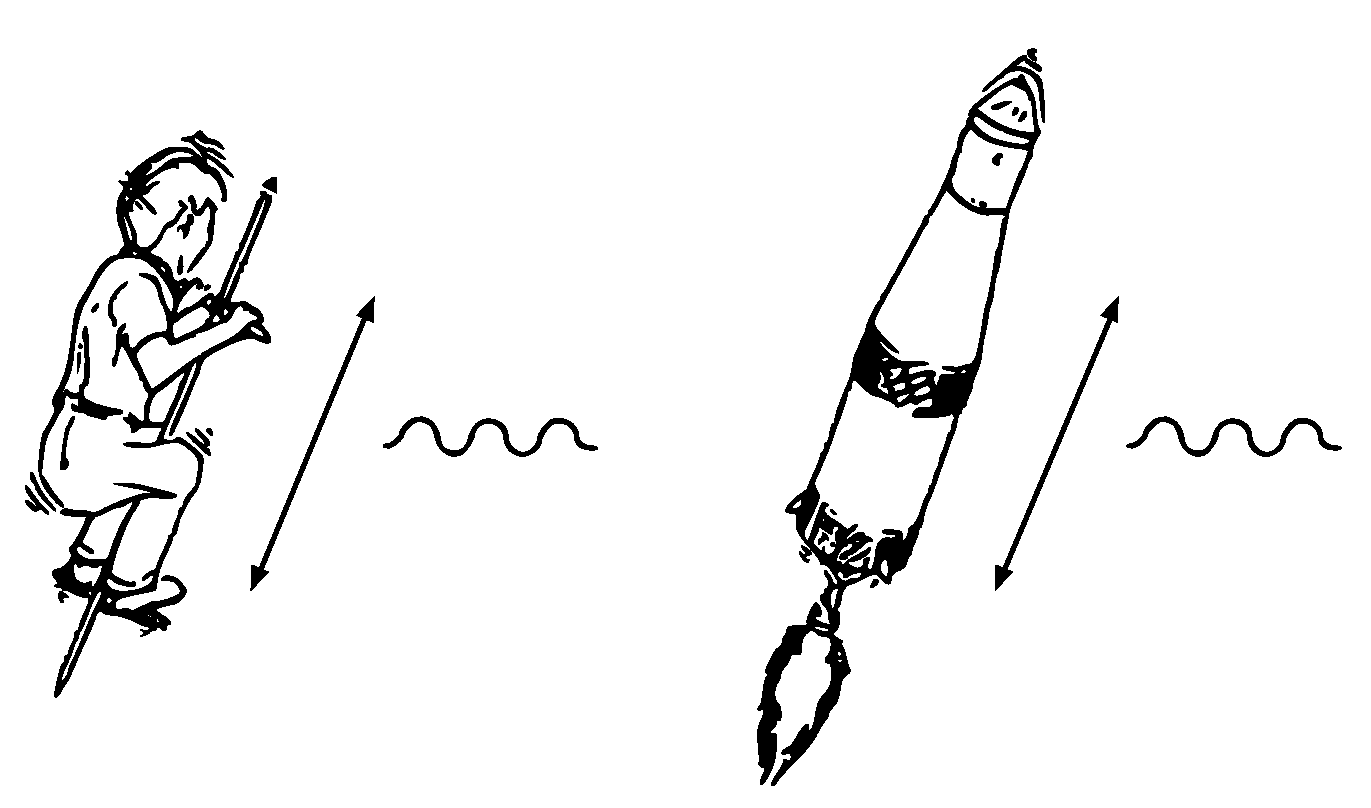
\includegraphics[width=.65\linewidth]{POGO-Analog}
  \caption{POGO比拟示意图}\label{POGO-Analog}
\end{figure}

\begin{figure}[th]
  \centering
  \includegraphics[width=.75\linewidth]{POGO-Typical.pdf}
  \caption{典型纵向耦合振动的时域历程}\label{Typical:POGO}
\end{figure}

纵观现代火箭工程发展史,POGO振动有害于人类航天飞行的典型例证当属美国土星V运载器的一系列发射经历\cite{Hill:1969, Rich:1969, Jarvinen:1970}。土星V运载火箭是美国最大的运载器,是美国国家航空航天局(NASA)在阿波罗计划和天空实验室两项太空计划中使用的多级可抛式液态燃料火箭。事实上,在其总共多达十三次的发射经历中,数次都受到了POGO振动问题的困扰\cite{Larsen:2008}。在1968年土星V编号AS-502次的发射过程中,液体火箭一级推进器(图\ref{SaturnV-Stage1})在工作段105$\sim$140秒内发生了振动频率为5.3Hz,幅值约0.33g的POGO振动。振动导致了五个发动机推力不同步,最终使得飞船登月舱裙部壁板发生开裂。同年十二月发射的土星AS-503,在发动机关机前50秒出现了振动频率为18Hz的POGO振动。事后调查表明,此次主发动机机架与贮箱底部产生的谐振虽然没有传递到火箭壳体,但是已经非常接近简体结构的设计强度极限。在1969年第AS-507次飞行中,液体火箭二级发动机在工作期间出现了四次严格意义上的POGO 振动,所幸最终都被结构系统的非线性效应所遏制。然而,在1970年土星V执行阿波罗13号任务的时候(AS-508),严重的POGO振动导致主发动机机架产生了频率为16Hz,加速度高达68g的失稳现象。由于燃烧室内压力脉动过于剧烈,火箭中部的5号推进器在二级火箭燃烧过程中发生了提前关闭(图\ref{SaturnV-Stage1}),最终导致登月任务被迫放弃,调查发现发动机机架总共被拉长了约7.6厘米。除此之外,宇宙神、大力神和雷神等航空运载器也都在各自发射过程中出现了或多或少的POGO振动\cite{Walker:1964, Wagner:1970, Oppenheim:1993};而法国钻石B火箭更是在其初次发射的五次飞行中都遇到了POGO振动,并且箭体上部分位置的振动量级已然高达足以导致运载器或者卫星结构发生破坏的20$\sim$30g\cite{Dordain:1974}。反观我国的航天事业,在2003年运载火箭长征2F第五次飞行中,遥测数据与宇航员的感受均显示一级助推器飞行末期火箭产生了比较强烈的振动\cite{Ma-Daoyuan:2010, Rong-Kelin:2011}。

\begin{figure}[t]
  \begin{center}
  \begin{minipage}{.47\linewidth}
    \includegraphics[width=\linewidth]{SaturnV-Stage1.jpg}
    \caption{土星V一级推进器 S-IC}\label{SaturnV-Stage1}
  \end{minipage}
  \begin{minipage}{.47\linewidth}
    \includegraphics[width=\linewidth]{SaturnV-Stage2.jpg}
    \caption{土星V二级推进器提前关闭}\label{SaturnV-Stage2}
  \end{minipage}
\end{center}
\end{figure}

POGO振动的危害性主要表现在如下几个方面\cite{Rubin:1970, Wang-Qizheng:1999}:
\begin{enumerate}[leftmargin=\parindent, align=parleft, labelindent=0pt, labelwidth=*]
\item 可使运载器结构系统产生过大的动载荷,造成火箭有效载荷部分损坏,影响主要任务的完成。如法国的“钻石B”运载火箭。
\item 管路系统产生的脉动压力和脉动流量可以导致运载火箭性能降低,造成任务失败。由于燃烧室压力的剧烈振荡导致出现虚假的推进剂耗尽指示信号,致使发动机过早关车。如美国的“大力神”二号任务失败,“土星V/阿波罗13”运载火箭第二级性能大大降低。
\item 增加运载器结构载荷,使有效载荷重量受到限制,而不得不重新设计结构。如美国的“雷神/阿金纳”火箭重新设计了“阿金纳”的结构。
\item 可以导致仪器、惯性仪表、设备和卫星所不允许的振动环境条件。如“雷神/阿金纳”运载火箭“阿金纳”级上的仪器设备需按较大的正弦振动等级重做安全鉴定。
\item 可以产生宇航员所不能允许的振动条件,使得宇航员的生理系统失调、身体不适,进而不能正常工作。如“双子星座/大力神”运载火箭的宇航员视力模糊,感到不舒服。
\end{enumerate}

根据NASA等机构对人体的测试表明\cite{Creer:1960, Burton:1988, Davis:2008}:垂直状态下正常人体所能承受的G力极限为5g,经过训练的宇航员可以短时承受正9g的最大加速度;在水平方向上,早期实验表明未经训练的人员在20g的加速度下只能坚持少于十秒的时间,10g可以支持一分钟,6g状态则能够维持十分钟。一般来说,短暂的“红视症”(Blackout,负G力)与“黑视症”(Redout,正G力)只是人体自我保护机制产生的警讯,用以警告人体已经濒临极限。倘若继续维持甚至增加G力,脑部将再因保护机制而停止工作产生昏厥,此时位于空中的飞行器即有极度危险;接着,当G力超过人脑所能负荷极限时,人脑将因长时间过度缺氧或充血的血管破裂而造成永久性伤害,最严重的即是因脑部严重损坏而死亡,或是脆弱的内部组织因持续遭受高G力而产生破裂,造成严重出血并危及生命。

可以看出,能否成功抑制甚至消除POGO振动已经成为当代航天运载器的重要设计指标之一,也是人类能否进行宇航飞行的前提之一。所以,目前基本上所有研究大型液体火箭的国家都对这种振动给予了相当大的重视和研究力度。因此,在我国大力发展宇航事业的重大契机下,针对POGO振动稳定性方面的理论分析也变得更加紧迫和必要。

\section{纵向耦合振动问题的主要机理分析}
\label{sec:POGO_Mechanicsm}
从本质上讲,POGO振动是一种由于火箭结构系统和管路推进系统发生相互作用而引起的不稳定振动。这种振动带有明显的流固耦合低频振动特征,属于不稳定的闭环自激振动\cite{Rubin:1973, Doiron:1977, Huang-Huaide:1987}。

\begin{figure}[h]
  \centering
  \includegraphics[width=.6\linewidth]{Struture-Feedline-Interaction-Diagram.pdf}
  \caption{POGO振动示意框图}\label{Interaction-Diagram}
\end{figure}

除去一种不常见的增压气体耦合POGO振动\cite{Rubin:1970},典型的POGO闭环振动究其原因可以归纳为如下过程(图\ref{Interaction-Diagram}):在大型液体运载火箭飞行的过程中,燃烧剂和氧化剂输送管路内的液路压力和流量会因为火箭结构系统的扰动而产生脉动。此脉动量经过不同管路元件的层层传递,最终将会到达液体火箭燃烧室,进而引起发动机产生推力脉动。此外,在燃烧剂和氧化剂的输运过程中,管路系统也会由于液体和管壁发生流固耦合作用而产生作用于结构系统上的额外反馈力\cite{About:1987, Paidoussis:1993}。所以当发动机推力脉动,联合上述管路系统反馈力,作为外界扰动力反作用于箭体结构时,火箭结构系统和管路推进系统两者就有可能因为固有频率相接近而产生不断放大耦合作用,从而导致液体推进火箭产生自激的纵向不稳定振动\cite{Rubin:1970, Oppenheim:1993}。

\begin{figure}[!htb]
  \centering
  \includegraphics[width=\linewidth]{telemetry-typical.pdf}
  \caption{土星V箭体加速度传感器数据}\label{telemetry-typical}
\end{figure}

参考POGO振动的发生机理并结合国内外大量的飞行遥测数据\cite{Feng-Zhenxing:1981},可以知道这种不稳定振动的发生频率大多与火箭结构系统的低阶纵向振动频率较为接近,其产生和发展过程也表现的十分突然和强烈。事实表明,POGO振动可能发生在液体火箭飞行过程的各个时刻,一次发射也确实可能会出现多次的POGO 振动\cite{Larsen:2008}。然而,由于液体火箭飞行过程是一个持续的变结构参数过程,并且箭体结构在发生较大变形时所引起的非线性效应会打破上面描述的这种频率耦合,所以即使出现POGO 现象,箭体振动的幅值也不会一直发散,而是在其响应时间的历程记录曲线上会出现一个先增大后减小的“鼓包”,典型的遥测POGO振动图像如图\ref{telemetry-typical}所示。鉴于POGO振动从发生到完全消失的时间可能长达数十秒,并且由其引起的箭体纵向振动加速度幅值可能在有效载荷处高达十几甚至几十倍于重力加速度,所以POGO振动对于液体火箭所造成的影响需要根据这种自激振动的量级及持续的时间来进行评价\cite{Wang-Qizheng:1999}。



\section{本文的主要工作}

\begin{figure}[!b]
  \centering
  \includegraphics[width=.85\linewidth]{Inter-connect.jpg}
  \caption{神舟十号与天宫一号交汇对接示意图}\label{China-Manned-Flight}
\end{figure}

液体火箭纵向耦合振动问题是一个相对古老却又富含新鲜挑战和契机的复杂系统问题。在我国大力发展航空事业的今天(图\ref{China-Manned-Flight}),更被赋予了深层次的时代意义。传统的液体火箭POGO稳定性分析方法主要分为了矩阵法、单传法和临界阻尼法\cite{Wang-Qizheng:1999}等几类。这些方法都需要先计算出耦合系统的闭环或者开环传递函数,然后通过对系统传递函数进行特征值求解或者绘制Bode和Nyquist图等手段来进行POGO稳定性分析。不过,由于耦合系统的传递函数通常都包含了一些复杂的非线性函数,所以POGO稳定分析的理论难点其实可以被归结为如何快速精确地计算出复杂传递函数的特征值这一经典问题。以矩阵法为例,由于系统反馈力传递矩阵中的元素包含了超越函数和高阶多项式,所以需要对不对称的复数传递矩阵进行非线性复特征值求解,而通常这种非线性方程的求解过程都十分困难并且容易漏根\cite{Dennis:1983, Golub:1996}。正是考虑到此类特征值问题的复杂性,Oppenheim\cite{Oppenheim:1993}等人如前所述,尝试了利用有限元法对管路系统进行直接建模。事实证明,这种方法在处理简单液路元件的组装计算方面确实具有着很高的可操作性和精确度。然而,由于管道内的流体运动问题归根结底是一个复杂的非线性问题\cite{Munson:1990, Paidoussis:1993, Morand:1995},所以当简单流体模型不能够精确描述管路系统传递关系,而研究者们必须要考虑诸如边界层效应,甚至湍流等复杂流体运动的时候,经典的有限元方法就必须被进一步拓展才能适应研究需要,而这种扩展可能相比于直接求解非线性特征值问题更加棘手。除此之外,由于流体单元本构关系的构建严重依赖于液路元件实验参数(如液路惯性,阻抗等)的精确标定,而相比于直接测定各类液路元件的工作参数,标定管路系统的总体反馈力传递函数可能会显得更加方便并且直接。所以,本文在POGO稳定性求解方法的研究方面,直接针对于管路系统的反馈力传递函数展开分析,开辟了另外一种与液路元件有限元组装法平行的POGO振动问题快速特征值求解方法。

为了解决上述主要问题,本文将研究工作分为了以下三个部分:

\begin{enumerate}[label=\textbf{\Roman*.}, align=left, leftmargin=0pt, listparindent=\parindent, itemindent=!, labelwidth=\parindent, labelsep=0pt, itemsep=1em]
\litem{集中参数模型的POGO稳定性分析(第二章)} 本章主要介绍了液体火箭结构系统和管路推进系统典型液路元件的集中参数模型建模方法,发展了一种基于矩阵法和有理分式拟合法的耦合系统快速特征值求解算法。首先推导了各类管路元件上下游脉动压力、流量之间的传递函数关系,结合发动机燃烧室的压力平衡条件与贮箱底部实际边界条件,综合分析出了管路系统反馈于结构系统的力传递函数。接下来,利用快速特征值求解方法,将包含超越函数的管路推进系统反馈力传递函数等效变换为与结构动力学方程一致的形式,通过求解矩阵特征值问题确定了耦合系统的动力学稳定性问题。最后,通过与传统矩阵法进行计算结果和效率方面的比对,验证了该方法的可靠性和高效性。
\litem{基于三维带液贮箱模型的POGO稳定性分析(第三章)} 为了更好的模拟火箭贮箱内液体和结构系统之间的流固耦合效应,引入液体火箭贮箱的三维轴对称模型建模方法,并利用虚质量法对贮箱内的液体进行动力学比拟。发展后的三维带液贮箱模型为管路系统提供了更为科学和精确的入口端边界条件,可以同样利用第二章中描述的管路系统类结构化建模方法,结合MSC.Nastran提供的传递函数TF卡建模工具,将拟合完毕的管路系统传递函数与不同类型的结构系统模型进行耦合计算。通过直接计算耦合系统的复特征值问题,可以方便的得知耦合系统的POGO稳定性。此外,计算过程还考虑了POGO稳定性分析中的另外一项关键性技术,即结构系统阻尼特性的识别和建模。带液贮箱的模态实验表明:在满箱、半箱和空箱等不同状态下,火箭结构系统的阻尼特性存在着较大差异,且半箱状态下结构阻尼较其他状态有明显增大。通过调整贮箱干/湿面材料随时间变化的比例阻尼系数,计算模型成功模拟了上述模态实验结果。最终,通过与实际火箭发射的遥测数据进行对比,证明了本套方法可以快速准确的得出POGO出现时间和振动特性。
\litem{液体火箭POGO稳定性参数分析及传递特性分析(第四章)} 通过比较不同工况下液体火箭POGO稳定性分析结果,本章首先揭示了耦合系统特征值与管路系统关键参数(如蓄压器容积等)之间的相互联系。分析表明,作为POGO抑制器的蓄压器,其容积变化能够显著影响液体火箭管路系统的固有频率,继而改变耦合系统的POGO稳定性。此外,通过比较不同类型液体火箭的历史遥测数据,可以发现有效载荷(如卫星等)的实际振动状态与液体火箭整体POGO振动的强弱并不存在简单的线性关系,单纯的耦合系统特征值计算并不能完全展现液体火箭各处的真实振动状态。文章最后指出,若要使得POGO稳定性分析能够给予未来的发射任务以实质性指导意见,还需综合考虑耦合系统的加速度传递特性分析。
\end{enumerate}

\input{Chapters/Chapter1} % Introduction and background theory

\input{Chapters/Chapter2} % Calculation Method and Result

\input{Chapters/Chapter3} % Experiment Data and Analysis

\input{Chapters/publishing}
%----------------------------Appendix-------------------------------!
\appendix  

\renewcommand{\thechapter}{附录{\Alph{chapter}}}

%\chapter{公式推导}
%----------------------------Back Matter-------------------------------!
\backmatter{}

\phantomsection
\addcontentsline{toc}{chapter}{\bibname}
\bibliographystyle{FDUbib}
\bibliography{Bibliography}
%\nocite{*}

\backchapter{致谢}



感谢赵凯锋导师指导,特别是最后阶段对论文和答辩报告幻灯片提出的修改意见。感谢王美玲师姐在我刚来实验室时的帮助,特别是在我研一时候组织的激光物理读书会开启了科研的大门。也感谢魏丽花师姐,优美的歌声不会忘记。在和廖康佳师兄对物理问题的讨论中,他独到的见解经常让我有超出预期的收获。感谢张桂迎师兄,他大量的文献阅读量使得在和他的讨论中,能够得知许多工作组目前在做的工作方向和最新进展,推荐文献以供学习研究。并且在生活中也给我许多指导。

感谢我在研究生阶段初期选课期间给我们授课的物理系各位老师,以及在课堂上认识的同学们。老师知识渊博,对于教学有着自己的思路和方式,非常真诚,做出了许多工作让学生尽可能多的理解;有幸认识了一群真正喜欢物理,并愿意做物理的同学们。在观察他们与老师的讨论中和与他们的讨论中,感受到执着和智慧,对待知识精益求精。

这里特别感谢徐建军老师,有幸选修徐老师的几门课,在他的引导下与和同班许多同学的讨论中好好学了两门课,感到自己进步好多,对物理的感觉建立起来。同样需要特别感谢吴赛骏老师,让我看到一流科研工作者的科研精神和风貌,实验室外的交流中学到了课本上不会讲的学习方法和感悟,回答了长期困扰自己的许多问题,让我有醍醐灌顶的感觉。

感谢现代物理研究所的每一位同学,每个同学身上都有闪光点,让我知道自己的不足和努力方向;

如果复旦是形容词,那么一定可以用来形容他们。

感谢现代物理研究所的杨明杰老师、杨柳老师、封娅娅老师、王冕老师及査老师对我毕业办理手续过程中提供的支持和帮助。感谢其他老师让我加快成长的速度,增长了我的阅历和见识。

最后感谢自己的父母,前十八年你们的养育工作已经顺利完成,剩下一棒就交给我自己了。

\clearpage
\printindex
\end{document}
